\documentclass[11pt]{article}
\pdftrailerid{}
\pdfinfoomitdate=1
\pdfsuppressptexinfo=-1
\usepackage[T1]{fontenc}
\usepackage[utf8]{inputenc}
\usepackage{lmodern}
\usepackage[margin=1in]{geometry}
\usepackage{amsmath,amssymb,amsthm,mathtools,bm}
\usepackage{graphicx,booktabs,enumitem,microtype}
\usepackage{needspace}
\usepackage{tikz}
\usetikzlibrary{arrows.meta,positioning,fit}
\usepackage[nottoc,notlof,notlot]{tocbibind}
\PassOptionsToPackage{hyphens}{url}
\usepackage[hypertexnames=false,hidelinks,bookmarksnumbered]{hyperref}
\usepackage[capitalise,noabbrev,nameinlink]{cleveref}
\newtheorem{theorem}{Theorem}[section]
\newtheorem{lemma}[theorem]{Lemma}
\newtheorem{proposition}[theorem]{Proposition}
\newtheorem{corollary}[theorem]{Corollary}
\theoremstyle{definition}
\newtheorem{definition}[theorem]{Definition}
\newtheorem{assumption}[theorem]{Assumption}
\theoremstyle{remark}
\newtheorem{remark}[theorem]{Remark}
\DeclareMathOperator{\Var}{Var}
\DeclareMathOperator{\Cov}{Cov}
\DeclareMathOperator{\sd}{sd}
\DeclareMathOperator{\tr}{tr}
\DeclareMathOperator{\supp}{supp}
\numberwithin{equation}{section}
\allowdisplaybreaks[2]
\setlength{\emergencystretch}{1.5em}
\hypersetup{pdftitle={The low-temperature Sherrington--Kirkpatrick fluctuation scale},pdfauthor={OpenAI}}
\title{The low-temperature Sherrington--Kirkpatrick\\ fluctuation scale}
\author{OpenAI}
\date{September 24, 2026}
\begin{document}
\maketitle
\begin{abstract}
For the zero-field Gaussian Sherrington--Kirkpatrick model at every fixed inverse temperature $\beta>1$, we prove that the standard deviation of the log partition function is $n^{1/6+o(1)}$. The same exponent describes its typical centered absolute fluctuations, establishing the predicted one-sixth exponent in this regime.
\end{abstract}
\section{Introduction}\label{sec:introduction}
Let $(g_{ij})_{1\le i<j\le n}$ be independent standard Gaussian random variables. For a fixed inverse temperature $\beta>1$, define
\[
 H_n(\sigma)=\frac{\beta}{\sqrt n}\sum_{1\le i<j\le n}g_{ij}\sigma_i\sigma_j,
 \qquad Z_n=2^{-n}\sum_{\sigma\in\{-1,1\}^n}e^{H_n(\sigma)},
 \qquad F_n=\log Z_n.
\]
The normalization of the spin sum changes $F_n$ by a deterministic constant and therefore has no effect on centered fluctuations.

\begin{theorem}\label{thm:main}
For every fixed $1<\beta<\infty$,
\[
 \sd(F_n)=n^{1/6+o(1)},\qquad \Var(F_n)=n^{1/3+o(1)}.
\]
More explicitly, for every $\eta>0$ there is $n_0(\beta,\eta)$ such that
\[
 n^{1/6-\eta}\le\sd(F_n)\le n^{1/6+\eta}
 \qquad(n\ge n_0(\beta,\eta)).
\]
Moreover, for every $\eta>0$,
\[
 \mathbb P\!\left(n^{1/6-\eta}\le|F_n-\mathbb EF_n|
                         \le n^{1/6+\eta}\right)\longrightarrow1.
\]
\end{theorem}
For the free-energy density $F_n/n$, the standard-deviation and typical-magnitude exponents are $-5/6$, and the variance exponent is $-5/3$. Multiplication by the fixed physical factor $-1/\beta$ has no effect on these exponents. Theorem~\ref{thm:main} concerns power exponents; it gives neither a limiting law nor a nonzero constant prefactor. The temperature is fixed throughout, with no uniform conclusion as $\beta$ approaches $1$ or infinity.

\subsection{History and significance}
The Sherrington--Kirkpatrick model \cite{SK1975} separates two questions:
the limiting free energy and its fluctuations between disorder samples.
Parisi introduced the hierarchy of order parameters underlying the
variational prediction for the first \cite{Parisi1979}.
Guerra and Toninelli \cite{GuerraToninelli2002} established the
thermodynamic limit by Gaussian interpolation, and Guerra's variational
bound \cite{Guerra2003} and Talagrand's matching result
\cite{Talagrand2006} identified its Parisi value. Panchenko subsequently
established the formula for general mixed $p$-spin models, including odd
interactions \cite{Panchenko2014}. These results determine the leading
extensive term; the fluctuations studied here occur on a smaller scale.

The prediction of that scale has a separate history. Kondor's replica
expansion near the critical temperature \cite{Kondor1983} is the starting
point of the calculation described by Parisi and Rizzo
\cite{ParisiRizzo2008,ParisiRizzo2009}. Crisanti, Paladin, Sommers, and
Vulpiani \cite{CPSV1992} predicted a scale $n^{-5/6}$ for the physical
free energy per spin in the low-temperature, zero-field phase. At fixed
$\beta$, this corresponds to $n^{1/6}$ for the log partition function.
Parisi and Rizzo developed the associated rare-deviation calculation
through the low-temperature phase. Inferring typical fluctuations from
that calculation requires an additional matching assumption, discussed
in \cite[Section~VI]{ParisiRizzo2009}.
Theorem~\ref{thm:main} establishes the predicted one-sixth exponent with
arbitrarily small power slack, for every fixed finite $\beta>1$.

At fixed high temperature $0<\beta<1$, order-one Gaussian fluctuations
go back to Aizenman, Lebowitz, and Ruelle
\cite{AizenmanLebowitzRuelle1987}. Chatterjee's work on disorder chaos
and superconcentration \cite[Theorem~1.5]{Chatterjee2009} gives
$\operatorname{Var}(F_n)=O_\beta(n/\log n)$, and his later lower-bound
method proves constant-scale nonconcentration
\cite[Theorem~2.4]{Chatterjee2019LowerBounds}.
Chen and Lam obtained a critical-temperature variance upper bound of
order $(\log n)^2$ \cite{ChenLam2019Critical}. At the critical point,
Du and Huang subsequently proved variance $\frac16\log n+O(1)$ and
a Gaussian limit \cite[Theorem~1.3]{DuHuang2026Critical}.
Critical-window limit theorems concern temperatures approaching the
transition
\cite{ChengLiuShaoXu2026CriticalWindow}.

For the fixed low-temperature regime considered here, Aronow and Lopatto
\cite[Theorem~1.4]{AL2026} prove, for all sufficiently large $n$,
\[
 c_\beta n^{4/15}\le \operatorname{Var}(F_n)
                         \le C_\beta n^{7/15}.
\]
Their positive-transform and deviation estimates are a direct
antecedent of the present argument.

The structure of the scalar Parisi minimizer is also essential.
Auffinger and Chen established origin-support and regularity properties
\cite{AuffingerChenProperties2015}, and proved uniqueness through a
stochastic-control representation \cite{AuffingerChenUniqueness2015}.
Jagannath and Tobasco developed variational support and self-consistency
conditions \cite{JagannathTobasco2017}. After Zhou's interval-support
result near the critical temperature \cite{Zhou2025}, Lopatto
\cite[Theorem~1.1]{Lopatto2026} established interval support $[0,q_\beta]$
and the corresponding density structure at every fixed $\beta>1$.
We use this theorem together with the support self-consistency in
\cite[Lemma~2.2]{Lopatto2026}. The strictly positive initial density
needed here is then derived from scalar
diffusion identities and a strict fourth-derivative estimate in
Section~\ref{sec:profile}.

\subsection{Proof strategy and method ancestry}
Set $T=\beta^2$. We work with the completed covariance
\[
 \mathbb E[H_n^c(\sigma)H_n^c(\tau)]=\frac{nT}{2}R(\sigma,\tau)^2,
 \qquad R(\sigma,\tau)=\frac{\sigma\cdot\tau}{n}.
\]
Here $H_n^c=H_n+D$, where $D$ is an independent common Gaussian of
variance $T/2$, and $F_n^c=F_n+D$. This completion gives the displayed
quadratic covariance; the added noise is removed in the final step.

The quantitative target is a positive Laplace window for
$\log\mathbb E\exp\{s(F_n^c-\mathbb EF_n^c)\}$ when $s$ exceeds
$n^{-1/6}$ by an arbitrarily small fixed power of $n$
(Proposition~\ref{fl:laplace-window}). To compare these transforms,
we reveal Gaussian covariance in stages and integrate a stage at mass
$u$ by the operation $X\mapsto u^{-1}\log\mathbb E e^{uX}$, with
expectation at $u=0$. Nondecreasing paths specify the cumulative
interaction and external-field covariance. Copies of the spin system
can share selected stages of this revelation; their prescribed common
prefixes form the finite trees used in the proof.

This hierarchical framework belongs to the lineage of Parisi recursion,
Ruelle's cascades \cite{Ruelle1987}, and Gaussian interpolation
\cite{GuerraToninelli2002,Guerra2003}. The cavity variational principle
of Aizenman, Sims, and Starr \cite{AizenmanSimsStarr2003} is a further
antecedent for comparisons that remove or add sites. We construct the
finite positive transition laws used here directly.

The closest analytic predecessor is Aronow and Lopatto's combination of
a pinned Brascamp--Lieb variance estimate, optimized covariance
interpolation, and positive moments
\cite[Propositions~2.2--2.3 and Section~3]{AL2026}.
The extensions proved here concern paired interaction and field clocks,
local comparisons, fixed higher moments, and grouped replica tests at
the fluctuation scale. The continuous inverse-Hessian inequality is due
to Brascamp and Lieb \cite{BL1976}. Its application after pinning one
terminal spin configuration is proved in Section~\ref{sec:foundations};
the resulting moment estimate is for the full unconditioned planted
path, not for an arbitrary fixed prefix.

A global replacement of both hierarchical pressures by their scalar
Parisi limits loses too much at this scale. Instead,
Section~\ref{sec:comparisons} optimizes short covariance comparisons
over a nondecreasing overlap quantile. The resulting error consists of
overlap variance and the mismatch between that quantile and the mean
overlap. Under comparability of mass and overlap above the scale being
tested, projection and pinned moment estimates make these errors small
in every fixed moment at selected split levels. The polynomial saving
can be chosen independently of that fixed moment order.

Section~\ref{sec:cavity} turns these estimates into a scalar description
of the mean overlap. Removing one spin produces a susceptibility
correction that is too large under an absolute term-by-term bound.
Additional test replicas give a finite system of identities whose
iteration cancels that correction. For a block already containing
observed replicas, the signed attachment contributions are summed
before absolute values are taken. The number of test factors and the
iteration depth remain fixed as $n$ grows. This gives the cubic
one-site closure of Proposition~\ref{prop:cavity-closure}, including
the uniform version needed for moving split locations.

Section~\ref{sec:profile} uses that closure and the comparison's first
variation to determine its small-mass profile. A limiting scalar
equation and a nonnegative variational potential exclude gaps in the
rescaled overlap distribution, forcing a positive linear profile.
The estimates hold in both mass and overlap coordinates, so an interval
of negligible mass cannot conceal a gap of appreciable overlap length.
The same section identifies macroscopic limits with the unique Parisi
minimizer; its control proof follows the strict-convexity method of
Auffinger and Chen \cite{AuffingerChenUniqueness2015}.

The local arguments assume regularity above the scale being tested.
Section~\ref{sec:regularity} removes this assumption by finite
propagation. A failure is examined at a scale with a regular outer
region. Sufficient comparison strength there already contradicts the
direct profile result. In the remaining case, a stronger local
comparison is constructed. If its error bound holds, agreement with
the original comparison yields the same contradiction; if it fails,
the next comparison has an error budget larger by a fixed power of $n$.
A fixed number of repetitions exhausts the admissible range.
Figure~\ref{fig:proof-order} records this alternative.

\begin{figure}[htbp]
\centering
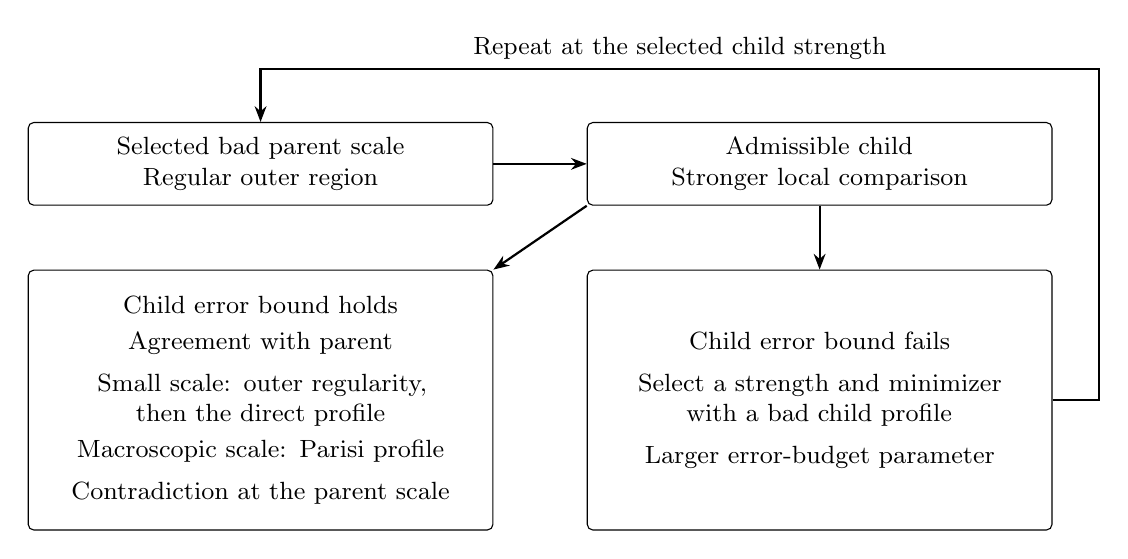
\begin{tikzpicture}[
 box/.style={draw,rounded corners=2pt,align=center,font=\small,
             text width=5.55cm,inner sep=5pt,minimum height=1.05cm},
 branch/.style={box,minimum height=3.3cm},
 flow/.style={-{Stealth[length=2mm]},thick}]
\node[box] (bad) at (0,0)
 {Selected bad parent scale\\Regular outer region};
\node[box] (child) at (7.1,0)
 {Admissible child\\Stronger local comparison};
\node[branch] (success) at (0,-3.0)
 {Child error bound holds\\[2pt]
  Agreement with parent\\[4pt]
  Small scale: outer regularity,\\
  then the direct profile\\[2pt]
  Macroscopic scale: Parisi profile\\[4pt]
  Contradiction at the parent scale};
\node[branch] (failure) at (7.1,-3.0)
 {Child error bound fails\\[4pt]
  Select a strength and minimizer\\
  with a bad child profile\\[4pt]
  Larger error-budget parameter};
\draw[flow] (bad.east) -- (child.west);
\draw[flow] (child.south west) -- (success.north east);
\draw[flow] (child.south) -- (failure.north);
\draw[flow] (failure.east) -- (10.65,-3.0) -- (10.65,1.2)
 -- node[above,font=\small] {Repeat at the selected child strength}
 (0,1.2) -- (bad.north);
\end{tikzpicture}

\caption{A selected bad parent scale has a regular outer region. The diagram
concerns the remaining weak-strength case; a direct profile test
already excludes sufficient local strength. Child-error success gives
agreement. At a scale tending to zero, this supplies child outer
regularity for the small-scale direct test; at a macroscopic scale,
the Parisi profile applies instead. Either profile contradicts the
parent failure (Lemma~\ref{reg:successful-child}). Child-error failure
selects a strength and minimizer, and then the next bad scale. Each
child raises the error-budget parameter by a fixed power of system
size. The covariance budget preserves admissibility, while this growth
exhausts the allowed error range after a fixed number of steps
(Proposition~\ref{reg:finite-propagation}). This propagation is separate
from the local finite-degree cavity recursion.}
\label{fig:proof-order}
\end{figure}

Finally, Section~\ref{sec:fluctuations} applies the resulting comparisons
to obtain the positive Laplace window. A positive transform alone does
not control variance or typical magnitude. Following the exponential
augmentation argument of \cite[Proposition~5.1]{AL2026}, we add an
independent rate-one exponential variable to $F_n^c$. Gauge symmetry
and Pr\'ekopa's marginal theorem \cite{Prekopa1973} give a log-concave
density. Its moment and small-ball bounds convert the Laplace window
into the standard-deviation and typical-magnitude assertions. Removing
the added exponential and Gaussian variables completes the proof.

\subsection{Conventions}
All constants may depend on the fixed $T$. Small auxiliary exponents are chosen first and held fixed as $n\to\infty$. Assertions along test sequences permit passage to subsequences, but never an $n$-dependent iteration depth. We write $A\lesssim B$ for an inequality with a constant independent of $n$, and $A\asymp B$ when both inequalities hold. Dependence on a fixed moment order is indicated by a subscript. A polynomial saving means a factor $n^{-c}$ for some fixed $c>0$; logarithmic losses are absorbed only after this saving has been established.

\tableofcontents
\section{Gaussian hierarchies and their calculus}\label{sec:foundations}

We construct the probability spaces and calculus for the next two sections.
Pressure differentiation turns covariance perturbations into overlap
errors in Section~\ref{sec:comparisons}; moments on one planted path
control those errors, and the finite-tree calculus organizes the
fixed-degree cavity expansions of Section~\ref{sec:cavity}.
Throughout this section
$n$ is a positive integer and the prior on $\{-1,1\}^n$ is uniform. All
expectations include both the Gaussian variables and the indicated spin
draws. The normalized planted law and its deterministic-weight variance
estimate follow the framework of \cite[Section~2 and Proposition~2.2]{AL2026}.
We prove the higher-moment and finite-tree extensions needed here.

\subsection{Finite hierarchies and conditional covariances}

Put $y(\sigma)=\sigma/\sqrt n$ and
$R(\sigma,\tau)=y(\sigma)\cdot y(\tau)$. The two feature maps
\[
 \phi_b(\sigma)=\frac{\sigma\sigma^{\mathsf T}}{\sqrt{2n}},
 \qquad \phi_h(\sigma)=\sigma
\]
take values in Euclidean spaces of dimensions $n^2$ and $n$, respectively.
Their inner products are $nR^2/2$ and $nR$, and their squared norms are
$n/2$ and $n$. The use of all ordered spin products is harmless and makes
the covariance realization immediate.

For the moment let $b,h$ be nonnegative nondecreasing step functions on
$(0,1)$. Choose a common partition
\[
 0=m_0<m_1<\cdots<m_L<m_{L+1}=1,
 \qquad b(u)=b_j,\quad h(u)=h_j
 \quad(m_j\leq u<m_{j+1}).
\]
Set $b_{-1}=h_{-1}=0$. Write $Z_j$ for independent feature-space Gaussian
vectors having coordinate variances $b_j-b_{j-1}$ in the first feature
space and $h_j-h_{j-1}$ in the second. Zero variances are permitted.
For a combined external field $z=(z_b,z_h)$ define
\[
 F_L(z)=\log\left(2^{-n}\sum_\sigma
       e^{z_b\cdot\phi_b(\sigma)+z_h\cdot\phi_h(\sigma)}\right),
 \qquad
 F_{j-1}(z)=\frac1{m_j}\log\mathbf E e^{m_jF_j(z+Z_j)}
 \quad (j=L,\ldots,1),
\]
and $F_{-1}(0)=\mathbf E F_0(Z_0)$. Thus the operation at mass zero is
expectation. Set
\[
 f_n(b,h)=\frac1n F_{-1}(0)-\frac{b_L}{4}-\frac{h_L}{2}.
\]
Common linear spin sources may be included in every terminal partition
function. A source coupled to $y$, used only for differentiation and then
set to zero, will be called a normalized spin source.

The associated planted law is constructed forwards. Draw $Z_0$ from its
Gaussian law. Conditional on $G_{j-1}=\sum_{i<j}Z_i$, draw $Z_j$ with
density
\[
 \exp\{m_j[F_j(G_{j-1}+Z_j)-F_{j-1}(G_{j-1})]\}
\]
relative to its Gaussian law. Finally draw $\sigma$ from the Gibbs law
in the field $G_L$. These are normalized transition kernels. At a
specified split, replicas share the prefix and then use conditionally
independent copies of all subsequent transitions. A finite deterministic
tree of such splits defines a probability law, even when some split
masses coincide or some covariance increments vanish. At a jump we
specify whether the split is before or after the increment. Repeated
empty steps allow these conventions to be recorded in a common partition.

Let $\mathcal F_u$ be the prefix sigma-field after the revelation specified
at $u$. For $m_j\leq u<m_{j+1}$ it includes $G_j$. Define
\[
 \begin{gathered}
 X_u=\mathbf E[y\mid\mathcal F_u],\qquad
 C_u=\mathbf E[yy^{\mathsf T}\mid\mathcal F_u]-X_uX_u^{\mathsf T},\\
 S_u=\mathbf E|X_u|^2,\qquad
 B_u=\mathbf E\bigl\|\mathbf E[yy^{\mathsf T}\mid\mathcal F_u]\bigr\|_{\rm HS}^2,
 \qquad D_u^2=B_u-S_u^2,\\
 L_u=y\cdot X_u-\tfrac12|X_u|^2.
 \end{gathered}
\]
Here and below conditional expectation given a prefix means conditioning
on its entire sigma-field.

\begin{lemma}[Source derivatives]\label{lem:found-source}
The gradient of a continuation in a source coupled to a bounded feature
$\phi$ is the conditional mean of $\phi$. Its Hessian is the sum of the
remaining conditional martingale covariance increments, weighted by the
mass of each transition, with mass $1$ for the final spin draw. In
particular, the Hessian $H_u$ in a normalized spin source satisfies
\[
 uC_u\preceq H_u\preceq C_u.
\]
If $y_1,y_2$ are independent continuations from the prefix at $u$, then
\[
 \mathbf E(y_1\cdot y_2)=S_u,\qquad
 \mathbf E(y_1\cdot y_2)^2=B_u,
\]
and hence $D_u$ is the standard deviation of this overlap. Moreover,
\[
 D_u^2=\operatorname{Var}(|X_u|^2)
       +2\mathbf E[X_u^{\mathsf T}C_uX_u]
       +\mathbf E\operatorname{tr}C_u^2.
\]
\end{lemma}

\begin{proof}
For $\mathcal T_m F=m^{-1}\log\mathbf E e^{mF}$, differentiation in any
external source gives
\[
 \nabla\mathcal T_mF=\mathbf E_m\nabla F,\qquad
 \nabla^2\mathcal T_mF=\mathbf E_m\nabla^2F
                  +m\operatorname{Cov}_m(\nabla F),
\]
where $\mathbf E_m$ is the normalized tilted expectation. At the
terminal spin sum the same formulas hold with mass $1$ and gradient
$\phi$. Iteration proves the claimed Hessian representation. More
explicitly, if $M_j=\mathbf E[\phi\mid\mathcal F_{m_j}]$ and
$C_L^\phi=\operatorname{Cov}(\phi\mid\mathcal F_{m_L})$, the Hessian at
the prefix indexed by $j$ is
\[
 \mathbf E\left[C_L^\phi+
   \sum_{k=j+1}^L m_k(M_k-M_{k-1})(M_k-M_{k-1})^{\mathsf T}
           \,\middle|\,\mathcal F_{m_j}\right].
\]
The same expression without the mass factors is the conditional
covariance of $\phi$. All remaining masses belong to $[u,1]$.
This proves the matrix inequalities. Conditional independence proves the
two overlap identities. Finally expand
$\|C_u+X_uX_u^{\mathsf T}\|_{\rm HS}^2$ and subtract $S_u^2$.
\end{proof}

\subsection{Pressure derivatives and the pinned moment estimate}

The three estimates needed later can be collected as follows. In the
first line, $db(u),dh(u)$ are variations in a parameter indexing paths;
they are not Stieltjes increments in $u$. In the second line $r$ increases
along the planted path. Its derivative is taken on absolutely continuous
parts. At a jump of the pair of clocks, fix the joint filling
$(b_-+t\Delta b,h_-+t\Delta h)$, $0\le t\le1$, at the jump's constant
mass. All intermediate revelations refer to this chosen filling.
The pressure and susceptibility estimates allow a common deterministic
source. The moment estimate is at zero deterministic external field,
under the full unconditioned law of one planted path and its terminal
spin configuration.
For every deterministic $k\in L^2(0,1)$ and $2\leq p<\infty$,
\begin{equation}
\begin{split}
 df_n&=-\tfrac14\int_0^1B_u\,db(u)\,du
       -\tfrac12\int_0^1S_u\,dh(u)\,du,\\
 \partial_rS_u&\geq n\,\partial_rh\,
                  \mathbf E\operatorname{tr}H_u^2,\\
 \left\|\int_0^1(L_u-\mathbf EL_u)k_u\,du\right\|_p^2
     &\leq c_p\left\|\int_0^1 k_u^2W_u\,du\right\|_{p/2},
 \qquad W_u=(y-X_u)^{\mathsf T}H_u(y-X_u),\\[-2pt]
 &\hspace{100pt}\mathbf EW_u=\mathbf E\operatorname{tr}(H_uC_u).
\end{split}\tag{1}\label{eq:1}
\end{equation}
One may take $c_2=1$ and $c_p\leq1+p^2/3$.

\begin{lemma}[Gaussian pressure differentiation]\label{lem:found-pressure}
The first two lines of \eqref{eq:1} hold for finite hierarchies, including
degenerate Gaussian increments by continuity. In addition, for any common
external source and any two admissible step paths,
\[
 |f_n(b,h)-f_n(\widetilde b,\widetilde h)|
 \leq\tfrac14\|b-\widetilde b\|_{L^1}
        +\tfrac12\|h-\widetilde h\|_{L^1}.
\]
The bound is uniform in the source when the same self correction is used.
\end{lemma}

\begin{proof}
Consider first one feature map $\phi$ of constant squared norm $q$ and
its cumulative covariance clock $c_j$. Let
$A_j=\mathbf E|\mathbf E[\phi\mid\mathcal F_{m_j}]|^2$.
Gaussian heat differentiation of the increment $c_k-c_{k-1}$, followed by
the tilted chain rule through all earlier transitions, gives
\[
 \frac{\partial F_{-1}(0)}{\partial(c_k-c_{k-1})}
    =\tfrac12\mathbf E\{\operatorname{tr}H_k^\phi
                         +m_k|M_k|^2\}.
\]
For $k=0$ the second term is zero. The martingale decomposition in
Lemma~\ref{lem:found-source} gives the explicit telescoping sum
\[
 \mathbf E\operatorname{tr}H_k^\phi
     =q-A_L+\sum_{j=k+1}^L m_j(A_j-A_{j-1}),
\]
so the last derivative equals
\[
 \tfrac q2-\tfrac12\sum_{j=k}^L(m_{j+1}-m_j)A_j.
\]
Subtract $qc_L/2$ from $F_{-1}(0)$. On writing
$d(c_k-c_{k-1})=dc_k-dc_{k-1}$, the derivative becomes
$-\frac12\sum_j(m_{j+1}-m_j)A_j\,dc_j$.
For the matrix feature $A_j=nB_{m_j}/2$; for the field feature
$A_j=nS_{m_j}$. Dividing by $n$ proves the pressure formula. All spin
bounds used here remain true with an external source. Since $0\leq S,B\leq1$,
integration along the convex segment joining two monotone paths proves
the asserted Lipschitz bound.

To prove the second line, fill one Gaussian increment continuously at its
fixed mass $m$. Its continuation solves the backwards heat equation with
nonlinearity $m|\nabla F|^2/2$. Under the normalized planted transition the
driving Gaussian process acquires drift $m\nabla F$. Differentiating the
backwards equation cancels this drift in the stochastic differential of
the source gradient. Thus $X$ is a martingale throughout the filled
increment. Its diffusion coefficient against the spin field of clock
$h$ is $\sqrt n H$, since the actual field couples to $\sqrt n y$.
The independent matrix field contributes another positive semidefinite
quadratic variation. It\^o's formula therefore gives
\[
 d\mathbf E|X|^2
    =n\mathbf E\operatorname{tr}H^2\,dh
       +\mathbf E\|J_b\|_{\rm HS}^2\,db,
\]
where $J_b$ is the mixed Hessian for the matrix feature and normalized
spin source. The last term is nonnegative. Concatenation proves the
claim along the path and through filled jumps. The heat differentiations
may first be made with positive variances and then passed to zero
variance by dominated convergence of the finite Gaussian integrals.
\end{proof}

\begin{lemma}[Pinned moments for one planted path]\label{lem:found-moments}
At zero normalized spin source and with no other deterministic external
field, the last two lines of \eqref{eq:1} hold with $c_2=1$ and
$c_p\leq1+p^2/3$. All these moments concern one planted path and its
terminal spin, with the full, unconditioned prefix law.
\end{lemma}

\begin{proof}
Write all independent Gaussian increments as linear images of a standard
Gaussian vector $\xi$. Multiply their normalized transition densities
and the terminal Gibbs density, and then condition on the entire terminal
configuration $\sigma\in\{-1,1\}^n$.
Terms at neighboring levels cancel. Up to an additive constant, the
negative logarithm of the resulting density of $\xi$ is
\[
 U_\sigma(\xi)=\tfrac12|\xi|^2-\ell_\sigma(\xi)
                      +\sum_{j=0}^L(m_{j+1}-m_j)F_j(G_j),
\]
where $\ell_\sigma$ is linear. Each continuation is convex, by
Lemma~\ref{lem:found-source}. If $A_u$ is its Hessian in the underlying
drivers, then
\[
 Q:=\nabla^2U_\sigma=I+\int_0^1 A_u\,du\succeq I.
\]
Use a virtual normalized spin source $\lambda$. The joint Hessian of
the continuation in $(\xi,\lambda)$ has blocks
\[
 \begin{pmatrix}A_u&B_u^{\rm mix}\\
                 (B_u^{\rm mix})^{\mathsf T}&H_u\end{pmatrix}
 \succeq0.
\]
With the spin fixed, the driver gradient of $L_u$ is
$g_u=B_u^{\rm mix}(y-X_u)$. Positivity of this block matrix implies, for
every driver direction $v$,
\[
 |v\cdot g_u|^2\leq(v^{\mathsf T}A_uv)W_u.
\]
Put $G=\int_0^1k_ug_u\,du$ and $J=\int_0^1k_u^2W_u\,du$.
Cauchy--Schwarz in $u$ gives
\[
 |v\cdot G|^2\leq
   \left(\int_0^1v^{\mathsf T}A_uv\,du\right)J
   \leq(v^{\mathsf T}Qv)J.
\]
Taking $v=Q^{-1}G$ proves $G^{\mathsf T}Q^{-1}G\leq J$.

The classical Brascamp--Lieb variance inequality
\cite[Theorem~4.1]{BL1976} applies to
this finite-dimensional density: $U_\sigma$ is smooth, its Hessian is
bounded below by $I$, and it has Gaussian tails after a linear tilt.
All required derivatives have at most the integrable growth allowed by
this density; alternatively, one can first use smooth compactly supported
approximations. It yields the conditional variance bound by
$\mathbf E[J\mid\sigma]$.

There is no change of centering on removing the pin. For
$\eta\in\{-1,1\}^n$, the transformation
\[
 \sigma_i\mapsto\eta_i\sigma_i,\quad
 (Z_h)_i\mapsto\eta_i(Z_h)_i,\quad
 (Z_b)_{ij}\mapsto\eta_i\eta_j(Z_b)_{ij}
\]
is orthogonal in each Gaussian feature space, preserves the hierarchy,
and sends $X$ to $\eta X$. Consequently it preserves $L_u$ and $W_u$.
This group acts transitively on terminal spins. The conditional law of
$\int k_uL_u\,du$, as well as that of $J$, is therefore independent of the
pinned spin. In particular its conditional mean is its unconditional
mean. Brascamp--Lieb proves the assertion for $p=2$ with $c_2=1$.

Here is an explicit extension to all real $p>2$. Set
$A=\int k_u(L_u-\mathbf EL_u)\,du$. Apply the same variance inequality
to $|A|^{p/2}$, using smooth regularizations at zero when necessary.
H\"older's inequality gives
\[
 \|A\|_p^p\leq\|A\|_{p/2}^p
       +\frac{p^2}{4}\|A\|_p^{p-2}\|J\|_{p/2}.
\]
If $2<p\leq4$, the first term is bounded using
$\|A\|_{p/2}\leq\|A\|_2$. For $p>4$ use the previously established
bound at exponent $p/2$ and
$\|J\|_{p/4}\leq\|J\|_{p/2}$. If $\|J\|_{p/2}=0$, the variance bound
already gives $A=0$. Otherwise put
$t=\|A\|_p^2/\|J\|_{p/2}$ and $\alpha=p/2$. Then
\[
 t^\alpha\leq d^\alpha+(p^2/4)t^{\alpha-1},
 \qquad d=1\ (p\leq4),\quad d=c_{p/2}\ (p>4).
\]
This implies $t\leq d+p^2/4$: for $t\geq d$ divide by
$t^{\alpha-1}$, and for $t<d$ the claim is immediate. Induction down the
finite sequence $p,p/2,p/4,\ldots$ now gives $c_p\leq1+p^2/3$.
Finally, conditioning on the prefix gives
$\mathbf EW_u=\mathbf E\operatorname{tr}(H_uC_u)$.
All integrals are justified first for bounded $k$ and then by $L^2$
approximation; $|X|\leq1$ and $0\preceq H\preceq C\preceq I$ suffice
for this passage.
\end{proof}

\begin{remark}\label{rem:found-single-pin}
For each fixed enlarged tree, first marginalize the other branches and
apply Lemma~\ref{lem:found-moments} to the resulting single-path law.
Then combine its moment bounds by unconditional H\"older under the
positive tree law, and finally integrate the signed topology measure.
The lemma is not applied after spin-dependent reweighting or conditioning
on a fixed prefix; no joint-spin pinned inequality is used.
\end{remark}

\subsection{Signed replica sums at real masses}

The following convention permits covariance differentiation without any
integer-replica or analytic-continuation assumption. An observed tree has
a fixed finite set of labeled leaves, deterministic split masses, and
specified revelation sides. A new summation label is allowed to coincide
with an old leaf, to follow it for a time and then branch, or to branch
at an existing fork. The corresponding expectations are always ordinary
normalized planted expectations. Only the coefficients with which they
are summed may be signed.

\Needspace{3\baselineskip}
\begin{proposition}[Covariance differentiation]\label{prop:found-replica}
Let $K_\theta(u;\sigma,\tau)$ be an affine family of cumulative Gaussian
covariance kernels of a finite hierarchy. Assume that the independent
increment covariances are positive semidefinite throughout the parameter
interval. Let $V=\partial_\theta K_\theta$ and let $P$ be a fixed bounded
spin test on a fixed observed split tree. Then
\begin{equation}
 \frac{d}{d\theta}\nu_\theta[P]
      =\frac12\sum_{c,d}\nu_\theta[P V_{cd}].
 \tag{2}\label{eq:2}
\end{equation}
The signed sum includes coincidences with old labels and between $c,d$.
For distinct labels, $V_{cd}$ is evaluated at their common revelation;
on the diagonal it is evaluated at the terminal covariance. The exact
weights are the real-power weights described in the proof. A constant
diagonal contribution, independent of the summation label, sums to zero.
Conditional means in $P$ can be represented by independent additional
replicas at their specified prefixes before this formula is applied.
\end{proposition}

\begin{proof}
It is enough to prove the formula for a finite hierarchy with positive
masses and nondegenerate increments; degenerate cases follow by
one-sided limits. At a node with incoming mass $a$ and next child mass
$b$, let $I$ denote the next child integral. Without observations the
expression at this node is $I^{a/b}$. If $k$ distinguished children are
prescribed, normalization of the planted transitions gives precisely
\[
 I^{a/b-k}\prod_{i=1}^k I_i,
\]
where $I_i$ is the corresponding tested child integral. A general spin
test is a finite linear combination of products of single-slot tests, so
this identity also determines its expectation by linearity. This finite
expansion is used only for the identity, not to estimate its norm.

Gaussian differentiation at one covariance increment supplies two
derivative slots and a factor $1/2$. Above that increment ordinary chain
rules propagate the integral derivative; below it product and power
rules allocate the two field derivatives. A hit on an existing child
has multiplicity one. If $h$ distinct new children are used, the
power-rule coefficient is $(a/b-k)^{\underline h}$. Each new child
integral carries its incoming factor $b$, so its effective coefficient
is the polynomial
\[
 b^h(a/b-k)^{\underline h}
       =\prod_{j=0}^{h-1}\bigl(a-(k+j)b\bigr).
\]
This identity holds for the actual real masses. In particular it has no
division by a small mass. A double hit in the same child is retained as
such. The final spin summation is the same product calculation with
child mass $1$.

More explicitly, give every derivative slot a distinct label in a finite
set $S$, even when directions agree, and write $D_A=\prod_{s\in A}D_s$,
$D_\varnothing=1$, and $\alpha=a/b-k$. The labeled product rule is
\[
 D_S\!\left(I^\alpha\prod_{i=1}^k I_i\right)
 =\sum_{(S_1,\ldots,S_k,\pi)}
   \alpha^{\underline{|\pi|}}I^{\alpha-|\pi|}
   \prod_{B\in\pi}D_BI\prod_{i=1}^kD_{S_i}I_i.
\]
Here the $S_i$ are disjoint subsets assigned to existing children, and
$\pi$ is an unordered partition of their complement in $S$ into nonempty
blocks, one per new child. Thus no additional $|\pi|!$ occurs. Factoring
the incoming $b$ from every new-child derivative gives the polynomial
coefficients above; zero masses use these polynomial coefficients and
the one-sided limits of the normalized child laws. Recursing with these
labeled partitions proves equality of each final labeled-topology
coefficient for every order of allocating the slots, before any spin
expectation is evaluated. Coincident labels occupy one terminal node.
Consequently allocation order may be changed with any bounded function
of the final topology carried along, before taking absolute variation.

For completeness, at the root perform the calculation on
$e^{a_0F_{\rm root}}\nu[P]$ with an auxiliary incoming power $a_0$.
Set $a_0=0$ after differentiation. The derivative of the prefactor then
vanishes and the normalized expectation remains. This is an algebraic
identity in derivatives of positive real powers; there is no inference
from values at integer masses. Summing the changes of independent
covariance increments assigns to a pair the change accumulated along
exactly its shared prefix, which is $V_{cd}$. This proves \eqref{eq:2}.

The one-label sum at the root has total weight $a_0=0$, as can also be
seen directly in Lemma~\ref{lem:found-attachment}. Hence a constant
diagonal term multiplied by an old-label test sums to zero. A common
source differentiation uses one derivative slot in the identical
calculation. Auxiliary leaves representing conditional means may be
marginalized at any point because all their transitions are normalized.
\end{proof}

\begin{lemma}[Attachment measures and row sums]\label{lem:found-attachment}
Fix an enclosing block of mass $a\in[0,1]$ containing $r\geq1$ observed
leaves. After grouping placements which induce the same extended tree,
one free summation label has the following signed attachment measure:
\begin{enumerate}[label=(\roman*)]
\item weight $+1$ for coincidence with each observed leaf;
\item measure $-dm$ on every occupied open edge, parameterized by its
      increasing mass coordinate;
\item weight $(1-d_v)u_v$ at an observed fork of mass $u_v$ with $d_v$
      occupied children, including an initial fork if present.
\end{enumerate}
The total signed mass is $a$ and the total variation is $2r-a\leq2r$.
For an empty block the first label has weight $a$. Consequently,
adjoining $k$ labels to a tree with $r\geq1$ old labels has total
variation at most
\[
 2^k r(r+1)\cdots(r+k-1).
\]
Adjoining $k\geq1$ labels in a previously empty block has variation at
most $a\,2^{k-1}(k-1)!$. These bounds are independent of the mass
partition. A free row whose summand is independent of the detailed
attachment inside a block of mass $u$ collapses exactly to $u$ times that
summand.
\end{lemma}

\begin{proof}
At a node of mass $a'$ having $d$ occupied children of next mass $b'$,
the coefficient of a previously unoccupied child is $a'-db'$, by the
one-slot real-power rule. If $d=1$, consecutive refinements telescope to
the negative of the length of the occupied edge. When several occupied
children first separate at $u_v$, write the coefficient as its edge
part plus $(1-d_v)u_v$. At a terminal singleton the existing-label hit
has coefficient $1$. These are exactly the three listed contributions.

To compute their sum, let the occupied edge lengths be $\ell_e$.
Summing endpoint differences over the finite tree gives
\[
 \sum_e\ell_e+\sum_v(d_v-1)u_v=r-a.
\]
Indeed each terminal contributes $1$, the initial point contributes
$-a$, and at a fork the endpoint contributions equal
$-(d_v-1)u_v$. All contributions except the $r$ coincidences are
nonpositive. Their signed sum is $a$, and their total absolute sum is
$r+(r-a)$. If there is no occupied child, the one-slot coefficient is
simply $a$. Insert further labels sequentially and apply the variation
bound to the enlarged occupied tree. The row-sum assertion follows
before taking absolute values from the total signed mass calculation.
Empty covariance steps merely subdivide edges and change none of these
identities.
\end{proof}

\begin{remark}[What a small mass does and does not imply]
The first entry into an empty block of mass $u$ costs a factor $u$.
Likewise departures on an initial interval of length $u$ have total
variation at most a constant, depending on the old leaf count, times
$u$. Subsequent fixed numbers of allocations retain this factor by
Lemma~\ref{lem:found-attachment}. However, the coefficient
$a-kb$ need not be $O(a)$ if $b\gg a$. A small enclosing mass alone
does not supply a factor to every ungrouped term. For two slots in an
empty block, the two different-child coefficient is $a(a-b)$ and the
same-child contribution on a constant test is $ab$. Their signed total
is $a^2$, whereas their absolute sum need only be $O(a)$. All small-mass
savings below use an actual first entry or an exact row collapse.
\end{remark}

\begin{lemma}[Densities of split levels]\label{lem:found-split-density}
Fix a finite observed tree with at most $q$ leaves and allocate at most
$k$ new labels. Apart from coincidences and atoms at specified old forks
or cuts, the split mass of any specified pair involving a new label has
a Lebesgue density with total variation bounded by a constant $C_{q,k}$.
The same statement holds when some old fork masses are themselves
integrated against a measure of bounded density, with the resulting
bound multiplied by that density bound. These assertions concern the
signed attachment measure and its variation, not the size of a
spin observable at a pointwise split level.
\end{lemma}

\begin{proof}
Allocate the specified pair before the other new labels, using equality
of the underlying finite product derivatives to reorder the allocations.
If one label is old, its non-atomic separation from the new label occurs
on an occupied edge and has density of absolute value $1$; there are at
most a number of edges depending on $q$. Old forks give precisely the
listed atoms. If both labels are new, first place one of them. A fork
created by a placement on an edge already has a bounded mass density.
The second label either separates on an edge, attaches at an old fork,
or attaches at this newly created fork. The last coefficient is bounded
by the number of occupied children, because its mass is at most $1$.
It therefore preserves the density bound in that variable. Coincidences
are kept separate. All remaining allocations have bounded total
variation by Lemma~\ref{lem:found-attachment}. Integration over an old
fork variable with bounded density is the same argument followed by
Fubini. The reordering was an exact identity before any absolute values
were taken, so it introduces no cancellation assumption in the final
variation estimate.
\end{proof}

\begin{lemma}[Uniform Taylor bounds]\label{lem:found-taylor}
Under the hypotheses of Proposition~\ref{prop:found-replica}, suppose
$P$ uses at most $q$ labels and $|V(u;\sigma,\tau)|\leq M$. For each
fixed integer $j\geq1$ there is $C_{q,j}<\infty$, independent of the
number of covariance steps, such that
\[
 \left|\frac{d^j}{d\theta^j}\nu_\theta[P]\right|
       \leq C_{q,j}M^j\|P\|_\infty.
\]
More precisely the derivative is an integral over a signed measure of
extended trees with uniformly bounded total variation, of expectations
of $P$ times $j$ covariance insertions, with the factor $2^{-j}$.
H\"older's inequality can therefore be applied to these integrands
under their genuine probability laws. If $P\geq0$, then
\[
 \left|\frac{d}{d\theta}\nu_\theta[P]\right|
        \leq C_{q,1}M\nu_\theta[P],
\]
and hence
\[
 e^{-C_{q,1}M|\theta-\theta'|}\nu_{\theta'}[P]
 \leq\nu_\theta[P]
 \leq e^{C_{q,1}M|\theta-\theta'|}\nu_{\theta'}[P].
\]
The assertions require that the test, including any scalar centers in
it, be fixed during the interpolation. For parameter-dependent tests
the ordinary product-rule derivatives must also be included.
\end{lemma}

\begin{proof}
Iterate \eqref{eq:2}. Affineness makes every covariance insertion fixed,
so the $j$th derivative has $2j$ additional labels and $j$ insertions.
Lemma~\ref{lem:found-attachment} bounds the variation of the resulting
measure by a constant depending only on $q,j$. This proves the first
two assertions, including Taylor's integral remainder. For a nonnegative
old-label test, each extended law has the same old-label marginal.
Consequently $\nu_\theta[|P V_{cd}|]\leq M\nu_\theta[P]$ for every
attachment, giving the differential inequality. Integrating it, or using
the integral form of Gr\"onwall's inequality when the expectation
vanishes, proves the comparison.
\end{proof}

\begin{corollary}[Source derivative bounds]\label{cor:found-source-bounds}
For fixed $n$, every derivative order of a continuation in bounded
feature directions has a bound independent of the mass partition,
uniform over the external source and the admissible bounded covariance
clocks. The bound depends only on the order and the suprema of the
feature directions.
\end{corollary}

\begin{proof}
The first derivative is the conditional feature mean. Differentiate it
with the one-slot version of Proposition~\ref{prop:found-replica}, and
repeat. Every additional derivative introduces one bounded feature and
one summation label. Lemma~\ref{lem:found-attachment} bounds each
successive attachment measure. A continuation beginning at a prescribed
prefix is treated as a rooted hierarchy by adjoining empty earlier
steps; its prefix is a deterministic external source. This makes the
same argument applicable without any lower bound on its first mass.
\end{proof}

\subsection{Cut truncations and conditional couplings}

We record the precise finite-tree facts needed when a free row is
replaced by a row truncated at a cut. A detailed attachment of a new
label $r$ is truncated at $t$ as follows. If it already departs from the
old tree before $t$, nothing is changed. Otherwise retain its old
ancestor through the prescribed revelation at $t$ and then draw its
continuation independently of the old descendants. Thus deeper
placements in the same occupied block at $t$ give the same truncated
law. The old-label marginal is always unchanged.

\begin{lemma}[Variation of a cut layer]\label{lem:found-cut-truncation}
Fix an old tree with at most $q$ leaves in a block of mass $U$, and a
free row label $r$ in that block. Let $U\leq v\leq w\leq\min(2v,1)$.
The difference of its signed row tests truncated at $w$ and at $v$ can,
after exact grouping of the deeper placements, be written as a signed
combination of pairs of planted laws with total coefficient variation
at most $C_qv$. In each pair the old-label tree is the same, and only
the coupling of $r$ to one occupied descendant subtree after the
revelation at $v$ differs. One may take $C_q=12q$.

The statement remains true when the row is multiplied by a bounded
coefficient depending on the fixed old topology, multiplied into the
bound by its supremum. For the exact collapse of deeper placements this
coefficient, and all scalar centers in the row test, must be independent
of $r$'s detailed attachment beyond the truncation cut.
Allocation-order symmetry carries the full topology coefficient with it;
it does not establish the independence required for a free-row collapse.
At each recursion generation, freeze the previously generated topology,
its coefficients, and earlier scalar centers before introducing fresh
slots. A current coefficient depending on the row's deeper placement
must remain explicit until eliminated or estimated. Only after this
row calculation may the enlarged topology be frozen for the next
generation.
\end{lemma}

\begin{proof}
Contributions departing before $v$ are identical and cancel. There are
at most $q$ occupied subblocks at either cut. Inside an occupied subblock
at $w$, every deeper placement gives the same $w$-truncated expectation,
so its signed sum is exactly $w$ by
Lemma~\ref{lem:found-attachment}. These collapsed tails have total
absolute coefficient at most $qw\leq2qv$. Departures on edges between
$v$ and $w$ have total length at most $q(w-v)\leq qv$. Fork atoms in
this layer have total absolute weight at most
$w\sum(d_v-1)\leq2qv$. Treat forks lying exactly on a cut with the
chosen revelation side; the same estimate covers them. Each of these
grouped contributions is the difference between retaining its indicated
coupling after $v$ and making $r$ independent at $v$; the old marginal
is preserved in both laws. Counting the two terms of these pairs gives
at most $10qv$, and $12qv$ allows terminal coincidences with either cut
convention. A terminal coincidence can occur in the layer only if
$w=1$, in which case $v\geq1/2$ and its unit weight is covered by the
same bound. Before that layer it is already included in a collapsed
tail. The asserted restriction on coefficients is exactly what is
needed for the identical-expectation grouping, and no further
independence from the old tree is used.
\end{proof}

\begin{lemma}[Centered coupling difference]\label{lem:found-coupling}
Consider either pair of laws in Lemma~\ref{lem:found-cut-truncation}.
Let $\mathcal G$ be the sigma-field generated by their complete common
prefix through the prescribed revelation at $v$, the realizations of
all old branches outside the affected descendant subtree after $v$,
and the deterministic old topology. No information from the continuation
of $r$ or from the affected old subtree after $v$ is included in
$\mathcal G$. Let $F$ be a function of $r$ and
this exterior information, and let $P$ be a function of the old
subtree and the exterior information. The two laws have the same
conditional marginal law of $F$ given $\mathcal G$ and the same
conditional marginal law of $P$ given $\mathcal G$. Write their common
conditional means as $\bar F,\bar P$. Their difference therefore obeys
\[
 (\mathbf E_1-\mathbf E_0)[FP]
   =(\mathbf E_1-\mathbf E_0)[(F-\bar F)(P-\bar P)].
\]
If $p^{-1}+p'^{-1}=1$, its absolute value is at most
\[
 \sum_{i=0}^1\|F-\bar F\|_{L^p(\mathbf P_i)}
                  \|P-\bar P\|_{L^{p'}(\mathbf P_i)}.
\]
Each centered norm is at most the corresponding norm of the difference
from an independent resampling with the same conditional marginal given
$\mathcal G$. Consequently uniform resampling bounds $A_v,B_v$ for
these two factors give a bound $2C_qvA_vB_v$ for the full cut layer.
\end{lemma}

\begin{proof}
Normalize and integrate every branch not retained in the conditioning.
Normalization of the transition kernels preserves the old subtree law.
It also gives the same single-continuation marginal for $r$, whether
$r$ follows an old branch for longer, coincides with an old terminal
label, or is made independent immediately after $v$. Conditional on
$\mathcal G$, the exterior information can change the distribution of
the shared prefix but not the normalized future kernels in the affected
subtree. This proves the two marginal assertions. Expand
$FP=(F-\bar F)(P-\bar P)+\bar FP+\bar PF-\bar F\bar P$;
the last three terms have equal expectations under the two laws.
H\"older's inequality gives the displayed bound after averaging over
$\mathcal G$. If $F'$ is an independent conditional copy, then
$F-\bar F=\mathbf E[F-F'\mid F,\mathcal G]$, so Jensen's inequality
gives the resampling bound; the argument for $P$ is identical.
Finally integrate against the coefficient measure of
Lemma~\ref{lem:found-cut-truncation}. Conditional bounds uniform in
the realized prefix are not needed: bounds in the displayed
unconditional $L^p$ norms suffice.
\end{proof}

\begin{lemma}[Boundary tests]\label{lem:found-boundary-tests}
Fix a cut $U$ and its old descendant blocks. Let $P$ be a polynomial of
fixed degree in overlaps between different blocks, centered by fixed
scalars, and in products of such overlaps with fresh auxiliary leaves
split at specified cuts. Assume that each overlap involving an affected
old subtree has its other endpoint outside that subtree. Bounded
coefficients may depend on the entire fixed old topology. All scalar
centers may be expectations on an earlier tree, provided they are held
fixed during the current row interpolation.

On resampling the affected subtree while retaining its prefix, only
the overlap factors crossing its boundary vary. If each such factor
has a resampling-difference bound in the required finite $L^p$ norm,
and the other factors have their required finite moment bounds, then
$P$ has the bound obtained by the product rule, with a constant
depending only on its degree, number of monomials, and coefficient bound.
In particular this property is preserved by multiplying the current
target test by centered overlaps to fresh auxiliary leaves, and by
introducing a fresh target block joined to an earlier target by one
overlap. Earlier target blocks may have several incident boundary
overlaps.
\end{lemma}

\begin{proof}
For a monomial use the exact identity
\[
 \prod_{i=1}^d A_i-\prod_{i=1}^d A_i'
    =\sum_{j=1}^d(A_j-A_j')
                   \prod_{i<j}A_i\prod_{i>j}A_i'.
\]
Factors supported in the exterior have $A_j=A_j'$. A fixed scalar center
also cancels from $A_j-A_j'$. Apply H\"older's inequality to each
remaining term, at exponents whose reciprocal sum is the reciprocal of
the desired exponent. Sum over the fixed finite collection of monomials.
This proves the norm transfer without any assertion that internal
overlaps are concentrated. The two stated operations introduce edges
between the current target and another block; they create no edge with
both endpoints in a single descendant block. The same argument
therefore remains applicable after each operation. The coefficient and
centering restrictions ensure that no unrecorded difference term is
introduced.
\end{proof}

\subsection{Passage to bounded monotone paths}

\begin{proposition}[Path limits]\label{prop:found-limits}
The preceding construction and estimates extend to bounded nonnegative
nondecreasing paths $b,h$ by step approximation. The limit is independent
of the approximations, provided the terminal clocks converge and the
before/after clocks at every specified cut converge to the specified
values. Planted expectations of bounded spin tests on a fixed finite
split tree with cuts before or after jumps, fixed-order source derivatives,
the signed calculus, and the mass-integrated pressure and moment formulas
have these limits. The susceptibility inequality holds on the continuous
parts, with nonnegative total increments of $S$ at jumps. For intermediate
cuts and the separate clock contributions inside a filled jump, use
approximations retaining the prescribed joint filling; no independence
from the choice of that filling is asserted. All constants in
the finite-tree variation and Taylor bounds are unchanged.
\end{proposition}

\begin{proof}
We give the details with $n$ fixed; no quantitative estimate uniform in
$n$ is inferred from this approximation argument. A bounded monotone
function has only countably many discontinuities. Choose step
approximations converging at its continuity points and retaining each
required side of the finitely many specified cuts. They converge in
$L^1$, and their endpoint clocks can be chosen to converge as well.
Lemma~\ref{lem:found-pressure} makes the self-corrected root values a
Cauchy sequence, uniformly over every common external source.

The same calculation applies to a continuation beginning at a fixed
cut $u$. Its future increment clocks are the cumulative clocks above
$u$ minus their specified values at that cut. Heat differentiation and
summation by parts give the same interior integral, together with an
initial boundary term. The latter is bounded by a constant depending
on $n$ times the difference of the two clocks at $u$, because all
feature means have norm at most their feature bound. Thus continuation
values converge uniformly in the external source whenever the clocks
at the cut converge; the bound consists of their $L^1$ differences
above $u$, their initial clock differences, and their terminal self
corrections. This also proves uniqueness of these limits.

Corollary~\ref{cor:found-source-bounds} bounds all source derivatives
uniformly over the approximations. Uniform convergence of values and
the bound on the next derivative imply convergence of any fixed
derivative by finite differences: approximate a derivative by a fixed
small difference quotient, pass to the limit in the quotient, and then
let its step tend to zero. Iterating this argument proves the claim
for mixed derivatives as well. In particular the limiting gradient and
Hessian are the conditional mean and weighted covariance limits.

To verify convergence of the probability laws, use independent standard
Brownian drivers for the finitely many features on each branch of the
fixed observed tree. Evaluate them at the deterministic $b,h$ clocks.
Continuity of Brownian paths gives convergence at every cut whose clocks
converge, including its prescribed side. Multiplication of normalized
transition densities telescopes on each edge exactly as in the pinned
calculation: the logarithm of the joint density is a finite sum of
endpoint and fork continuation terms and terminal Hamiltonians, minus
integrals of continuations along the edges in the mass coordinate.
The coefficients of endpoint terms are bounded in terms of the number
of observed leaves.

Here is a uniform integrable bound for this density. For fixed $n$ and
bounded clocks, terminal log partition functions are Lipschitz in the
feature source with fixed constant. The same is true of continuations
by the first derivative formula. Their values at source zero are
nonnegative and bounded by the annealed value, which is at most
$n(b(1-)/4+h(1-)/2)$. It follows that the absolute value of the
telescoped log density is at most
\[
 C_{n,q}\left(1+\sum_{\text{branches and features}}
                      \sup_{0\leq t\leq M}|B_t|\right),
\]
where $M$ bounds all clocks and $q$ is the fixed leaf count. The
exponential of this expression is integrable for a finite collection
of Brownian motions. Continuation convergence and dominated convergence
in the mass integrals therefore give almost sure convergence of the
densities and convergence in $L^1$. The same domination, together with
the source derivative bounds, applies to the differentiated observables
under consideration. This proves convergence of positive planted
expectations and their fixed-order source versions.

The attachment measure consists of finitely many fork and coincidence
atoms and Lebesgue measures on finitely many occupied edges, with
uniform total variation. At a Lebesgue placement, the clocks converge
outside a countable exceptional set. At an existing fork they converge
on the specified side by construction. Dominated convergence and
Lemma~\ref{lem:found-attachment} therefore pass every fixed finite
sequence of signed allocations to the limit. The same argument on an
affine interpolation segment passes fixed-order differentiation and
Taylor's integral remainder, since their variation bounds are uniform.
Exact permutation and row-sum identities survive because they held
before passage to the limit.

Finally $|L_u|\leq3/2$ and $0\leq W_u\leq4$. Thus the moment estimate
passes first for bounded deterministic weights and then for all
$L^2$ weights. For the clock identity, choose refinements that retain the prescribed
joint filling of every jump whose total clock size exceeds a cutoff,
and then let the cutoff decrease to zero. After the finitely many retained
jumps are separated, remove the remaining jumps temporarily. Their total
clock size tends to zero; the continuation and source-derivative estimates
above control this perturbation. The resulting clocks are continuous on
each interval between retained jumps, so their monotonicity gives uniform
clock convergence there. These estimates and Brownian continuity give
convergence of the quadratic-variation integrands, including within the
vanishing increments of the refinements, and hence of their Stieltjes
integrals. The uniform integrand bounds control the direct contribution
of the omitted jumps as well. At each retained jump the
prescribed joint filling fixes the separate clock integrals. Their sum
is the total nonnegative increment of $S$, independently of the filling.
Discarding this increment gives the susceptibility inequality on the
continuous portions. This proves the stated clock assertions without
claiming that the separate jump contributions are independent of their
joint filling.
\end{proof}

Henceforth all path quantities refer to these limits. The signed sums
are integrals of ordinary finite-tree expectations against the
attachment measures above. In particular all subsequent fixed-order
Taylor estimates have constants independent of how finely a path is
approximated.

\section{Optimized short comparisons}\label{sec:comparisons}

This section proves local estimates for a constrained comparison, including
an error estimate conditional on regularity outside the scale being tested.
The regularity assumption is stated each time it is used.  The later
propagation argument establishes it by a finite sequence of further
comparisons; none of the estimates below assumes the conclusion of that
argument.
The construction uses the optimized interpolation and pinned-field
averaging framework of \cite[Proposition~2.3 and Section~3]{AL2026}, with
the local strength profile and the scale-dependent constraints retained
throughout.

\subsection{Parameters and the constrained comparison}

Fix a sufficiently small constant $m>0$ and put $\delta=m/10000$.
All asymptotic statements concern $n\to\infty$ with these constants fixed.
The temperature, bounds on the total clocks, and fixed comparability
constants may enter implicit constants.  A polynomial saving means a
factor $n^{-c}$ for some fixed $c>0$.  Such a saving, unless otherwise
specified, is independent of each fixed moment order; the multiplicative
constant and the threshold in $n$ may depend on that order.  Factors denoted
by $n^{o(1)}$ can be bounded by $C_\epsilon n^\epsilon$ for any fixed
$\epsilon>0$.  We choose $\epsilon$ after the positive power margins in an
estimate have been fixed.  The estimates hold along arbitrary sequences
of parameters satisfying the stated assumptions, and hence also along
subsequences. We write $o_{\rm poly}(A)$ for a quantity bounded in
absolute value by $Cn^{-c}A$ for some fixed $c>0$. A bound $Y=O_p(A)$
means $\|Y\|_{L^p}\le C_pA$ at each fixed moment order under discussion.

A comparison call has parameters
\begin{equation}
 n^{-2/3+m}d\lesssim E\le n^{-1/2}d^2,
 \qquad a=\frac{\sqrt n E}{d},\qquad
 u_*=\frac1{nE},\qquad 0<d=O(1).
 \tag{3}\label{eq:3}
\end{equation}
The parameter $E$ sets the comparison-error budget, up to the fixed
power slack used below. The maximal covariance-removal strength is
$d^2$; at that strength the profile in \eqref{eq:6} changes scale near
radius $d$. The quantity $a$ is the corresponding lower direct-test
scale, while $u_*$ controls the smallest-mass constraints.
In particular $d\ge a\gtrsim n^{-1/6+m}$.  The working interval of masses
is $[u_0,1]$, where either $u_0=0$ or $u_0=o(a)$; changes made by this call
vanish below $u_0$.  Its endpoint clocks are denoted by $b_0,h_0$.  They are
uniformly bounded and nondecreasing on the working interval.  For the
subsequent profile argument the endpoint hypothesis is
\begin{equation}
 b_0(u)=T+o(z^2),\qquad h_0(u)=o(z^3)
 \quad\text{when }u\asymp z,\quad a\lesssim z\le1.
 \tag{4}\label{eq:4}
\end{equation}
This formulation is sequential: it holds on every such test sequence,
with any fixed comparability constants and with masses in the open
working interval.  In particular it implies uniform little-oh estimates
on each fixed compact scaled mass band, by choosing a violating point if
uniformity were to fail.

Choose $r_{\min}=0$ in the all-mass case.  In the case $u_0>0$ we may fix
any $0\le r_{\min}\le u_*/M(u_0)$.  The optimization variable is an
increasing onto quantile $r:[u_0,1]\to[r_{\min},1]$.  Its inverse
$\alpha$ satisfies $\alpha(r_{\min})=u_0$, $\alpha(1)=1$, and
\begin{equation}
 \begin{gathered}
 k(r)\le\alpha'(r)\le M(\alpha(r)),\qquad
 k(r)=\frac{n^\delta u_*^2}{(r+n^{2\delta}u_*)^2},\\
 M(u)=n^\delta\left[\frac{u+u_*}{L}
                  +\frac{d^3}{E}(u+u_*)^2\right],
 \qquad L=\min\left(u_*,\frac{a^3}{d^2}\right).
 \end{gathered}
 \tag{5}\label{eq:5}
\end{equation}
These are almost-everywhere constraints on Lipschitz functions, with a
strictly positive floor.  The inverse is therefore Lipschitz at fixed
$n$ as well.  The parameters in \eqref{eq:5}, including $r_{\min}$, remain
fixed when the strength is varied.

Fix once and for all a smooth function $f>0$ that equals $1$ in a
neighborhood of $0$, is comparable to $(1+\log t)/t$ for large $t$, and
whose logarithmic slope is nondecreasing from $0$ to $1$.  We require
$1-p\gtrsim[1+\log(1+t)]^{-1}$ for that slope.  Such a function is
obtained by choosing a smooth nondecreasing slope that is zero near zero
and equals $1-(1+\log t)^{-1}$ for all sufficiently large $t$, and then
integrating its logarithmic derivative.  Set
\begin{equation}
 \begin{split}
 e(r)&=\lambda f(\lambda r/d^3),\qquad 0\le\lambda\le d^2,\\
 \mathcal F_\lambda(r)
 &=f_n\bigl(b_0-e(r),h_0+e(r)r\bigr)
       +\frac14\int_{u_0}^1 e(r(u))r(u)^2\,du,
 \qquad \mathcal M_\lambda=\min_r\mathcal F_\lambda(r).
 \end{split}
 \tag{6}\label{eq:6}
\end{equation}
Here and below $e(r)$ in a clock denotes composition with $r(u)$, and
the changes in \eqref{eq:6} are zero below $u_0$.  We write
$p(r)=-re'(r)/e(r)$.  Thus $0\le p<1$,
$\partial_{\log\lambda}e=(1-p)e$, and $(re)'=(1-p)e\ge0$.
Consequently the comparison preserves monotonicity inside the working
interval.  A call at a fixed strength is admissible when the changed
clocks in \eqref{eq:6} are nonnegative and nondecreasing for every
quantile in \eqref{eq:5}, including across the boundary $u_0$.
An admissible sweep requires this for every strength in the sweep,
including zero.  The endpoints used later will satisfy these conditions.
A bare endpoint may instead have a field discontinuity at $u_0$ that
is repaired only at a fixed positive strength.  In that case the local
estimates concern the changed paths at that strength; the bare pressure
and a sweep from zero are not used.

\begin{lemma}[Existence and the optimized envelope]\label{comp:envelope}
For all sufficiently large $n$, the class \eqref{eq:5} is nonempty and
compact in the uniform topology of inverse quantiles.  The minimum in
\eqref{eq:6} is attained.  For an admissible sweep, $\mathcal M_\lambda$
is locally Lipschitz and nondecreasing in $\lambda$, equals the endpoint
pressure at $\lambda=0$, and is an upper bound for that pressure.
At almost every positive strength its upper derivative per unit
$\log\lambda$ is bounded, at any minimizer at that strength, by
\begin{equation}
 \frac14\int_{u_0}^1 e(r(u))
           \bigl[D_u^2+(S_u-r(u))^2\bigr]\,du.
 \tag{7}\label{eq:7}
\end{equation}
All moments in this formula are for the changed clocks in
\eqref{eq:6}.
\end{lemma}

\begin{proof}
We have $k\le n^{-3\delta}$ and $M\ge n^\delta$, while
\[
 \int_0^1 k(r)\,dr\le n^{-\delta}u_* =o(1),\qquad
 \int_{u_0}^1\frac{du}{M(u)}
 \le n^{-\delta}L\log\frac{1+u_*}{u_0+u_*}=o(1).
\]
The floor alone does not reach the prescribed terminal mass.  The cap
flow reaches it before the prescribed terminal radius.  Interpolating
controls in $\alpha'=k+w(M(\alpha)-k)$, $0\le w\le1$, gives a feasible
endpoint by continuity of the scalar flow; equivalently, interpolate the
travel time until the cap flow reaches mass $1$.  At fixed $n$ the
derivatives are uniformly bounded by $\max_{[u_0,1]}M$.  Uniform limits
preserve both differential inequalities in their integrated form, so
Arzel\`a--Ascoli gives compactness.  The positive floor preserves
invertibility.  Continuity of the pressure follows from the bounded
variation formula \eqref{eq:1}; this proves attainment.

For a fixed quantile, interpolate the amount of covariance removed from
$0$ to $e$.  The derivative of the pressure plus the corresponding
penalty is the integral of $[B-2rS+r^2]/4$ times the nonnegative strength
increment.  Since $B=S^2+D^2$, it is nonnegative.  This proves the
upper-bound assertion and monotonicity, including after minimizing.
At positive strength use an old minimizer as a competitor for a positive
increment of strength.  The same differentiation and
$\partial_{\log\lambda}e=(1-p)e\le e$ give \eqref{eq:7}.
Bounded spin moments give local Lipschitz continuity of the objective
uniformly over the compact admissible class, and hence of its minimum.
Integration of its almost-everywhere derivative is therefore legitimate.
The whole interval $0\le\lambda\le n^{-10}$ costs $O(n^{-10})$.
\end{proof}

\begin{definition}[Outer regularity]\label{comp:outer-regularity}
A minimizer has a regular outer region above $x$ if, for fixed positive
constants $c,C,C_0$, one has $cu\le r(u)\le Cu$ whenever
$u\ge C_0x$.  Enlarging the cutoff by a fixed factor gives the
equivalent comparison $\alpha(r)\asymp r$ in radius coordinates.  The
constants are independent of $n$.  No bound on a pointwise path
derivative is part of this definition.
\end{definition}

The eventual regularity assertion concerns every test scale
\begin{equation}
 n^\delta\frac{\sqrt n E}{\sqrt\lambda}\le x\le1.
 \tag{8}\label{eq:8}
\end{equation}
It will be proved after the profile analysis, by propagation from larger
scales.  In the present section it is a target range, not an assumption
already established at every minimizer.  Write
$A_\lambda=n^\delta\sqrt n E/\sqrt\lambda$.
If $x\ge A_\lambda$, then $x\gtrsim a$ and
$e(x)x^2\gtrsim n^\delta nE^2$: indeed
$\sqrt\lambda\sqrt n E\le d^3$, so the argument of $f$ at
$A_\lambda$ is at most $n^\delta$, and $re(r)$ increases.
Our local estimates require only $x\gtrsim a$ and
$e(x)x^2\gtrsim nE^2$, together with outer regularity when $x=o(1)$.

\subsection{First-variation geometry}

Define
\[
 G(r)=e(r)\left[(2-p(r))r-2(1-p(r))S_r-p(r)B_r/r\right],
\]
with the final term interpreted as zero in the neighborhood where $p=0$.
Subscripts $r$ here mean revelation at mass $\alpha(r)$.

\begin{lemma}[Contact, cap, and floor]\label{comp:geometry}
At a minimizer there is a continuous absolutely continuous potential
$H$ such that $H'=JG$ for a strictly positive factor $J$,
$\alpha'=M(\alpha)$ on $\{H<0\}$, and $\alpha'=k$ on $\{H>0\}$.
On a band where $\alpha+u_*$ varies by a bounded factor, $J$ has bounded
distortion after normalization at one endpoint.  On the contact set
$\{H=0\}$, almost everywhere,
\begin{equation}
 G=0,\qquad S'\lesssim n^{o(1)},\qquad S\le r.
 \tag{9}\label{eq:9}
\end{equation}
On an open cap component $\{H<0\}$ of radius length $\ell$,
\begin{equation}
 \begin{gathered}
 \Delta S\lesssim n^{o(1)}
        (\ell+r_{\min}\mathbf1_{\mathrm{initial}}),
 \qquad S\le r+\ell,\\
 |S-r|^2\lesssim n^{o(1)}
   \left[D^2+\ell^2+r_{\min}^2\mathbf1_{\mathrm{initial}}\right].
 \end{gathered}
 \tag{10}\label{eq:10}
\end{equation}
Here $\Delta S$ is the increase through the interior of the component.
On contact, $(S-r)^2\lesssim D^2$.  Every cap has
$\ell\lesssim n^{-\delta}L\log n$; if it is contained in a comparable
mass band $u\asymp v\gg u_*$, then
$v\ell\lesssim n^{-\delta}E/d^3$.  A noninitial cap on which $p=0$
throughout satisfies $|S-r|\le\ell$.  The total floor mass is at most
$n^{-\delta}u_*$.
\end{lemma}

\begin{proof}
Differentiating the objective with respect to its forward quantile gives
$\frac14\int G\,\Delta r\,du$.  The inverse variation is therefore
$-\frac14\int G\,\Delta\alpha\,dr$.  Write
$\alpha'=k+w(M(\alpha)-k)$ with $0\le w\le1$.  Its linearized
equation has fundamental factor
\[
 J(r)=\exp\left(\int_{r_{\min}}^r w(t)M'(\alpha(t))\,dt\right).
\]
Terminal preservation says
$\int(M-k)\Delta w/J=0$.  Integrating the first variation in the
opposite order gives a box-constrained linear functional with this one
linear constraint.  A scalar multiplier gives a function with derivative
$JG$, which must be nonpositive where $w=1$ and nonnegative where $w=0$.
Both signs of correcting endpoint variation exist: a feasible path
cannot be the pure floor or pure cap, as their travel times above show.
Thus the multiplier can equally be obtained by adding a correcting
variation and taking one-sided limits.  This proves the asserted rule.
Directional derivatives follow by the segment variation formula; the
fixed-$n$ inverse functions have dominated difference quotients.  Values
at jumps affect no integrals.  Moreover
\[
 \frac{M'(u)}{M(u)}\le\frac2{u+u_*},\qquad wM\le\alpha',
\]
which proves bounded distortion of $J$ on the stated bands.

The bracket in $G$ decreases with $p$, since its $p$ derivative is
$-[(r-S)^2+D^2]/r$.  At a noninitial left cap endpoint its limiting
value is nonpositive, and at the right endpoint it is nonnegative.
At radius $1$ the latter remains true because $S,B\le1$.
The right inequality implies $S\le r$ there and $pB\le2r^2$.
Use the right-end slope parameter at both endpoints.  If their radii
are comparable, subtraction of the inequalities, monotonicity of $B$,
and $pB\le2r_{\mathrm{right}}^2$ give
$2(1-p)\Delta S\le C\ell$.
If the radii are not comparable, $S\le r_{\mathrm{right}}\lesssim\ell$
suffices.  At an initial component use $S\ge0$, introducing only
$r_{\min}$.  Since $(1-p)^{-1}=O(\log n)$ on the polynomial scales
under consideration, this proves the first line of \eqref{eq:10}.

For the mismatch bound, the case $S>r$ follows from the right endpoint.
In a noninitial component with comparable endpoint radii, the left
inequality and monotonicity, followed by replacement of its radius by
the current radius, give
\[
 (r-S)\left[(2-p)+pS/r\right]\le C\ell+pD^2/r.
\]
When $S<r$, this gives $r-S\le C(\ell+D^2/r)$; splitting into
$D\ge r$ and $D<r$ proves the squared estimate.  Noncomparable and
initial components are covered by their length and wall terms.
The same calculation at $G=0$ proves $S\le r$ and
$(S-r)^2\lesssim D^2$ on contact.  At density points of the zero set,
difference quotients between adjacent zero-set points yield
$S'\lesssim(1-p)^{-1}$: the derivatives of $B$ and $p$ have favorable
signs, and $pB/r^2\le2$ there.  This proves \eqref{eq:9}.
The exceptional contact set has zero radius length and, since $\alpha$
is Lipschitz at fixed $n$, zero mass.

On a cap, $dr=du/M(u)$, so the two length bounds follow respectively
from the two positive terms of $M$.  If $p=0$, the endpoint signs say
$S_{\mathrm{left}}\ge r_{\mathrm{left}}$ and
$S_{\mathrm{right}}\le r_{\mathrm{right}}$, proving the sharper
mismatch statement.  Finally, floor mass is bounded by
$\int_0^1 k(r)\,dr\le n^{-\delta}u_*$.
\end{proof}

\subsection{Projection estimates and the raw-moment bootstrap}

Assume for now that $x=o(1)$, $x\gtrsim a$,
$e(x)x^2\gtrsim nE^2$, and the minimizer has a regular outer region
above $x$.  After a fixed enlargement of the cutoff, all bands below
are regular in both coordinates.  On the working interval
$\partial_r[h(\alpha(r))]\ge e(r)/O(\log n)$.
Hereafter $\partial_r h$ denotes this derivative of the clock pulled
back to radius coordinates. At regular scales $r\asymp u\asymp v$,
\begin{equation}
 u_*\ll x,\qquad
 M(O(v))\ll(nEv)^2\lesssim n e(v)v^4,
 \qquad n^{-1/6}\ll x.
 \tag{11}\label{eq:11}
\end{equation}
Every strict gain in this display is polynomial.  Indeed
\[
 \frac{u_*}{a}\lesssim n^{-3m},\qquad
 \frac{u_*^2d^2}{a^4}\lesssim n^{-6m},\qquad
 \frac{d^3}{n^2E^3}\lesssim n^{-3m}.
\]
For $v\gtrsim a$, dividing $M(O(v))$ by $(nEv)^2$ bounds the ratio by
$Cn^\delta$ times the sum of these three quantities.
The comparison with $ne(v)v^4$ follows because $e(r)r^2$ increases.
Monotonicity and the outer bounds also show that if one of $u,r$ is
$O(x)$, the other is $O(x)$.

\begin{proposition}[Raw moments]\label{comp:raw-moments}
For every fixed $p\ge2$, throughout the path, including masses below
the working interval,
\begin{equation}
 \|X_u\|_p\lesssim_p\sqrt{u+x},\qquad
 \|R_{\mathrm{split\ at}\ u}\|_p\lesssim_p u+x.
 \tag{12}\label{eq:12}
\end{equation}
The bounds also hold at intermediate clock revelations, with their
specified mass.  The norm of a random vector is its Euclidean norm
inside the $L^p$ norm.
\end{proposition}

We first establish a projection estimate that will also be used later.

\begin{lemma}[Projection after a field-clock interval]\label{comp:projection}
Let $V$ be a vector determined by outside branches and by data at or
before their fork with a branch $b$.  Conditional on this data, the
future of $b$ has its usual planted law.  Suppose a field-clock interval
after the fork has length $D_h$, with mass at least $v_->0$ throughout.
For even fixed $p\ge2$, the part of $V\cdot y_b$ left after projection
at the end of the interval satisfies
\begin{equation}
 \|V\cdot(y_b-X_{b,\mathrm{end}})\|_p
 \le C_p(\log n)^2\frac{\|V\|_p}{v_-\sqrt{nD_h}}.
 \tag{13}\label{eq:13}
\end{equation}
Here the masses and clock lengths used in the estimate are bounded
below by inverse powers of $n$.  Differences of two later projections
satisfy the same estimate up to a constant.
\end{lemma}

\begin{proof}
Condition on the outside data so that $V$ is fixed for the branch
calculation.  Put $Y=V\cdot y_b$ and $Y_t=V\cdot X_{b,t}$.
In field-clock time, the spin Brownian driver has planted drift
$t\sqrt n X_{b,t}$.  This follows on each filled increment from the
normalized exponential tilt and its logarithmic gradient; subdivision
gives the Brownian formulation.  Gaussian differentiation of the
telescoping planted density gives, for a subinterval $I$ and
$P=(Y-Y_{\mathrm{start}})^{p-1}$,
\[
 \mathbb E\left[P\int_I V\cdot(dG-t\sqrt n X_{b,t}\,dh(t))\right]
 =\sqrt n\int_I\mathbb E\left[
 P\left\{t(Y-Y_t)+\int_t^1(Y-Y_z)\,dz\right\}\right]dh(t).
\]
The terminal tilt contributes $Y$; the subsequent continuation terms
and the subtracted innovation drift contribute
$-\int_t^1Y_z\,dz-tY_t$.  Prefix-dependent parts of the test are fixed
before the subinterval, so no derivative of $V$ or
$Y_{\mathrm{start}}$ is taken.  This identity is first an ordinary
finite Gaussian integration by parts and then passes to filled clocks
by the path approximation already established.

For $z$ after the subinterval's start, conditional centering gives
\[
 \mathbb E[P(Y-Y_z)]
 =\mathbb E\left[
 \bigl((Y-Y_{\mathrm{start}})^{p-1}
       -(Y_z-Y_{\mathrm{start}})^{p-1}\bigr)(Y-Y_z)\right]
 \ge c_p\mathbb E|Y-Y_z|^p.
\]
This is the uniform monotonicity inequality for the odd power $p-1$.
Also $\|Y-Y_{\mathrm{end}}\|_p\le2\|Y-Y_t\|_p$ for earlier $t$.
The innovation on the left, divided by $\sqrt{h(I)}$, has norm at
most $C_p\|V\|_p$.  H\"older's inequality therefore gives the recursion
\[
 \|Y-Y_{\mathrm{end}}\|_p^p
 \le \frac{C_p\|V\|_p}{v_-\sqrt{nh(I)}}
       \|Y-Y_{\mathrm{start}}\|_p^{p-1}.
\]
Divide the given clock into $N=\lceil(\log n)^2\rceil$ equal pieces.
The coefficient is
\[
 \frac{C_p\sqrt N\|V\|_p}{v_-\sqrt{nD_h}}.
\]
Iteration raises the ratio of the initial bound $2\|V\|_p$ to this
coefficient to the power $(1-1/p)^N$.  If the ratio is larger than one
it is at most a fixed power of $n$, so its final power tends to one.
If it is smaller than one the assertion is already immediate.
This proves \eqref{eq:13}, with its harmless logarithmic allowance.
Conditional Jensen proves the assertion for later projections.
\end{proof}

\begin{proof}[Proof of Proposition~\ref{comp:raw-moments}]
\emph{Integrated susceptibility bound.}
Fix an integer $l\ge1$ and let
\[
 Q=\max\left(1,\sup_u
       \frac{\|X_u\|_{4l}}{\sqrt{x+u}}\right),
\]
including intermediate revelations and the final spin.  This is finite
at each fixed $n$.  We first bound the integrated weight in
\eqref{eq:1} on a small regular band of mass and radius comparable to
$v$.  Uniformly on a bounded enlargement of this band, choose $\rho$ so
that
\begin{equation}
 M(O(v))\rho\le n^{-c},\qquad
 ne(v)v^4\rho\ge n^c
 \tag{14}\label{eq:14}
\end{equation}
for a fixed $c>0$ independent of $l$.  For example take the geometric
mean between the reciprocal scales; \eqref{eq:11} gives the required
room, and $\rho=o(1)$.

We give the layer estimate first on a finite filled hierarchy, appending
the terminal spin as a martingale step of mass $1$.  In this paragraph
parentheses denote radius coordinates: $X(s)=X_{\alpha(s)}$,
$\mathcal F(s)=\mathcal F_{\alpha(s)}$, and likewise $H(s),W(s)$;
write $X(\dagger)=y$ and $\mathbb E_s=\mathbb E[\,\cdot\mid\mathcal F(s)]$.
Enclose the band in a radius interval $I=[r_-,r_+]$, with
$r_\pm\asymp v$ and $r_+<r_c/2$ for a fixed small $r_c>0$.
Its fixed enlargement is regular.  Put
\[
 \mathsf A_v=M(Cv),\quad \mathsf B_v=ne(v)v^4,\quad
 \rho=(\mathsf A_v\mathsf B_v)^{-1/2},\quad \eta=\rho v.
\]
By \eqref{eq:11}, with $\kappa=3m-\delta>0$,
$\mathsf A_v/\mathsf B_v\lesssim n^{-\kappa}$; hence
$\mathsf A_v\rho=(\mathsf B_v\rho)^{-1}\lesssim n^{-\kappa/2}$, as required
in \eqref{eq:14}.  Also $\mathsf A_v\ge n^\delta$, so $\rho=o(1)$.

For each $s\in I$, fork an independent continuation $b$ from the original
branch $a$.  On both branches use cuts
$t_0=s$, $t_1=s+\eta$, $t_2=2s$, then doubled radii up to the first
$t_J\in[r_c,2r_c)$, and $t_{J+1}=\dagger$.
Set $\Delta_i^a=X^a(t_{i+1})-X^a(t_i)$, and similarly for $b$.
There are $K=J+1=O(\log n)$ layers.  With
$w_0=w_1=s$, $w_i=t_i$ for $2\le i<J$, and $w_J=1$,
their largest masses $\mu_i$ satisfy
$\mu_i\lesssim w_i$ and $\|\Delta_i^{a,b}\|_{4l}\lesssim_l Q\sqrt{w_i}$.
For elementary martingale increments $d_\nu^b$ after the fork,
conditional orthogonality gives the indexed positive-semidefinite bound
\[
 H(s)=\mathbb E_s\sum_{\nu\text{ after }s}
        m_\nu d_\nu^b(d_\nu^b)^{\mathsf T}
 \preceq\sum_{j=0}^J\mu_j
        \mathbb E_s[\Delta_j^b(\Delta_j^b)^{\mathsf T}].
\]
Indeed cross terms between distinct elementary increments in each
block have zero conditional expectation.  Since
$y^a-X(s)=\sum_i\Delta_i^a$, scalar Cauchy--Schwarz yields
\[
 W(s)\le K\sum_{i,j=0}^J\mu_j\,
   \mathbb E_b[(\Delta_i^a\cdot\Delta_j^b)^2\mid a].
\]
Here conditioning on $a$ includes the common prefix; no coupling of the
auxiliary branches for different $s$ is needed.

For $(i,j)\ne(0,0)$ choose the branch carrying layer
$k=\max(i,j)$, taking either branch on a tie.  Condition on the entire
opposite branch and use its increment as the exterior anchor in
Lemma~\ref{comp:projection}.  The clock preceding the selected layer is
\[
 [s,s+\eta]\quad(k=1),\qquad
 [3t_k/4,t_k]\quad(2\le k\le J).
\]
Its masses are bounded below by $cw_k$, also for the terminal layer
because $t_J\asymp1$.  The field-clock length is at least
$c\rho ve(v)/\log n$: for $k=1$ this follows from
$\partial_r h\gtrsim e(r)/\log n$, and for $k\ge2$ from the same bound and
monotonicity of $re(r)$, with no factor $\rho$ needed.
All these scales are bounded below by inverse powers of $n$.
The opposite increment has norm at most $C_lQ\sqrt{w_k}$, even when
its endpoint is later than the fork, since it belongs to an independent
branch.  Equation~\eqref{eq:13} and conditional Jensen for later
projections therefore give
\[
 \mu_j\|\Delta_i^a\cdot\Delta_j^b\|_{2l}^2
 \le \frac{C_l(\log n)^5Q^2}{\rho nve(v)}.
\]
Conditional Jensen also bounds the $L^l$ norm of the corresponding
conditional square by this squared $L^{2l}$ norm.  Integrating over
physical mass $O(v)$ and summing the $K^2$ pairs, including the factor
$K$ above, bounds their total by
$C_l(\log n)^8Q^2v^4/(\mathsf B_v\rho)$.

For $(i,j)=(0,0)$ put
$q_s=\mathbb E_s|X(s+\eta)-X(s)|^2$ and
$Z=\sup_{r_-\le t\le r_++\eta}|X(t)|$ on the original path.
The integrand is at most $CvZ^2q_s$; changing coordinates costs only
$du\le \mathsf A_v\,ds$.  Doob's inequality gives
$\|Z^2\|_{2l}\le C_lQ^2v$.  To estimate the remaining integral, for
$\xi\in[0,\eta)$ let $r_j=r_-+\xi+j\eta$, retaining precisely the
$N=N(\xi)$ starting points in $I$ and their last endpoint
$r_N\le r_++\eta$.  Set
\[
 U_j=|X(r_j)|^2,\quad A_0=0,\quad
 A_{j+1}=A_j+q_{r_j},\qquad
 q_{r_j}=\mathbb E[U_{j+1}-U_j\mid\mathcal F(r_j)].
\]
Thus $A_{j+1}$ is $\mathcal F(r_j)$-measurable.  For $p=2l$,
$A_N^p\le p\sum_jA_{j+1}^{p-1}q_{r_j}$, and the exact identity
\[
 \begin{split}
 \sum_{j=0}^{N-1}A_{j+1}^{p-1}(U_{j+1}-U_j)
 ={}&A_N^{p-1}U_N-A_1^{p-1}U_0\\
 &-\sum_{j=1}^{N-1}(A_{j+1}^{p-1}-A_j^{p-1})U_j\\
 \le{}&A_N^{p-1}U_N
 \end{split}
\]
gives $\mathbb E A_N^p\le p\mathbb E[A_N^{p-1}U_N]$.
Consequently $\|A_N\|_{2l}\le2l\|U_N\|_{2l}\le C_lQ^2v$,
independently of the grid cardinality.  The shifted-grid identity
\[
 \int_Iq_s\,ds
   =\int_0^\eta\sum_{j=0}^{N(\xi)-1}q_{r_-+\xi+j\eta}\,d\xi
\]
and Minkowski give $\|\int_Iq_s\,ds\|_{2l}\le C_l\eta Q^2v$.
H\"older therefore bounds the integrated first-pair term by
$C_lv\mathsf A_v(Q^2v)(\eta Q^2v)=C_l\rho \mathsf A_vQ^4v^4$.

Combining the pairs, including their logarithmic multiplicities, gives
\[
 \left\|\int_{\mathrm{band}}W_u\,du\right\|_l
 \le C_l(\log n)^8
       \left[\mathsf A_v\rho Q^4+(\mathsf B_v\rho)^{-1}Q^2\right]v^4.
\]
All estimates use moments at most $4l$.  Include deterministic jumps
and intermediate cuts in the finite hierarchy.  An after-revelation
endpoint assigns its jump to the preceding block; a before-revelation
endpoint assigns it to the following block.  Equivalently insert both
ordered nodes, counting the jump exactly once.  The constants are independent of the
mesh and grid cardinality, so the established bounded-path approximation
passes to filled clocks at fixed $n$; the countable set of jump radii
does not affect the radius integral.  Absorbing logarithms, for example
with $c'=\kappa/4$, proves
\begin{equation}
 \left\|\int_{\mathrm{band}}W_u\,du\right\|_l
 \lesssim_l n^{-c'}(Q^4+Q^2)v^4,
 \tag{15}\label{eq:15}
\end{equation}
where $c'>0$ is independent of $l$.  The argument also bounds integrals
over subsets, since $W\ge0$.

\emph{Closing the moment estimate.}
For a regular small mass $u$, choose a future window of mass comparable
to $u$ at radii comparable to $u$.  Its means satisfy
$\mathbb EL_j=S_j/2\le Cu$.  Indeed this follows on nonfloor points
from Lemma~\ref{comp:geometry}; the floor has total mass $o(u)$, so
monotonicity permits looking ahead to a nonfloor point.  For $j\ge u$,
$2\mathbb E_uL_j=\mathbb E_u|X_j|^2\ge|X_u|^2$.
Apply \eqref{eq:1} and \eqref{eq:15} to the normalized window average.
Conditional Jensen yields
\[
 \||X_u|^2\|_{2l}\le Cu+C_l n^{-c''}Q^2u.
\]
For smaller masses, including $u<u_0$, choose a deterministic future
regular cut $t\asymp x$.  The identity
$X_u=\mathbb E[X_t\mid\mathcal F_u]$ and conditional Jensen give
\[
 \|X_u\|_{4l}^2\le\|X_t\|_{4l}^2
                    \le Cx+C_l n^{-c''}Q^2x.
\]
Macroscopic masses are bounded directly by $|X|\le1$.
Taking the supremum gives $Q^2\le C_l+C_l n^{-c''}Q^2$, which closes
for all sufficiently large $n$.  This proves the first bound of
\eqref{eq:12} for exponents divisible by four, and hence for every
fixed exponent.  It also removes $Q$ from \eqref{eq:15}.

\emph{The two-leaf overlap.}
If $u+x$ is bounded below, the overlap bound is immediate from $|R|\le1$.
Otherwise choose a regular radius $q=C(u+x)$, with $C$ fixed and
sufficiently large that $[q/2,q]$ is regular and lies after the fork.
Outer comparability and monotonicity permit this choice even when
$u<u_0$.  Write $X^a(q)=X^a_{\alpha(q)}$ and similarly for branch $b$.
The projected inner product has norm
$\|X^a(q)\cdot X^b(q)\|_p=O_p(q)$ by the bound just proved.

Decompose each leaf into its projection at $q$ and subsequent doubling
layers, ending with the terminal spin as in the susceptibility estimate.
Every product other than the two initial projections contains a later
layer of scale $w\ge q$.  An innovation interval before that layer has
mass at least $cw$ and field-clock length at least
$ce(w)w/\log n$.  The opposite branch supplies an exterior anchor of
norm $O_p(\sqrt w)$.  Lemma~\ref{comp:projection}, now without a
mass weight, bounds the product by
$C_p(\log n)^C/\sqrt{ne(w)w^2}$.
Since $e(w)w^2$ increases, summing the logarithmically many layer pairs
gives
\[
 \|R-X^a(q)\cdot X^b(q)\|_p
 \le\frac{C_p(\log n)^C}{\sqrt{ne(q)q^2}}
 =q\,\frac{C_p(\log n)^C}{\sqrt{ne(q)q^4}}
 =o_{\rm poly}(q),
\]
where \eqref{eq:11} supplies the last saving.  This proves the second
bound in \eqref{eq:12}.  All innovation intervals lie in the regular
region, including when the original fork is below the working interval.
\end{proof}

\begin{lemma}[Postprojection changes]\label{comp:resampling}
Suppose two leaves share only through a mass at most a fixed multiple
of $x_1$, where $x_1\ge x$.  If a projection or resampling is made after
a regular radius $v\ge Cx_1$, with comparable intervals fitting after
the fork and before that projection, the change in their inner product
caused by changing one endpoint has norm
\begin{equation}
 \frac{C_p(\log n)^C}{\sqrt{ne(v)v^2}}
 \tag{16}\label{eq:16}
\end{equation}
in every fixed $L^p$.  For an already projected anchor of norm
$O_p(\sqrt{x_1})$, the bound gains a factor $\sqrt{x_1/v}$.
\end{lemma}

\begin{proof}
Use the synchronized two-branch layer decomposition in the last part
of the preceding proof.  Every term involving the changed endpoint
contains an increment after its projection.  At the later layer of
scale $w$, the projection estimate gives
$C_p(\log n)^C/\sqrt{ne(w)w^2}$.  Monotonicity of $we(w)$ controls
the sum from its first scale $v$, up to logarithms.  For a fixed
projected anchor replace its raw $\sqrt w$ bound in
\eqref{eq:13} by $\sqrt{x_1}$.  Conditional Jensen covers replacement
by conditional projection, and two such replacements cover independent
resampling.
\end{proof}

\subsection{A split with uniform bounds in every fixed moment}

\begin{lemma}[Good split]\label{comp:good-split}
Suppose a regular band of mass and radius of order $v\ge Cx$ contains
a mass interval of length comparable to $v$ on which $S\asymp v$.
There are constants $c_1,c_2>0$, independent of each fixed moment order,
and a deterministic window of mass length $n^{-c_1}v$ with the following
properties.  Its fixed-factor enlargement has $S$ oscillation at most
$n^{-c_1/2}v$, and for every deterministic split in a fixed central
fraction of the window,
\begin{equation}
 \|R_*-S_*\|_p\le C_p n^{-c_2}v
 \tag{17}\label{eq:17}
\end{equation}
for all fixed $p\ge2$.  The window may be selected before the moment
orders or any later fixed recursion depth are chosen.  The constant
$c_1$ may be any sufficiently small positive constant.
\end{lemma}

\begin{proof}
Write $\theta=n^{-c_1}$, $\eta=n^{-c_1/2}$.  Among order
$\theta^{-1}$ disjoint buffered windows of mass length comparable to
$\theta v$, at most order $\eta^{-1}$ have $S$ oscillation larger
than $\eta v$, because the total increase is $O(v)$.  Choose one of
the remaining windows.  This is a deterministic selection involving
only $S$.  Fix past and future buffers of length comparable to
$\theta v$ surrounding a central region.

After the raw bootstrap, \eqref{eq:15} takes the form
$\|\int W\,du\|_q\le C_q n^{-\gamma}v^4$ for a $\gamma>0$
independent of fixed $q$.  Positivity of $W$ and \eqref{eq:1} give,
for the normalized $L$ average $A_J$ over either buffer,
\[
 \|A_J-\mathbb EA_J\|_p
 \le C_p n^{-\gamma/2+c_1}v=:C_p\zeta v.
\]
Let $t$ be a deterministic cut in the central region.  The exact
conditional identities give
\[
 2\mathbb E_t A_-\le|X_t|^2\le2\mathbb E_t A_+,
 \qquad
 |X_t|^2-2\mathbb E_t A_-
   =\operatorname{avg}_{s\in J_-}|X_t-X_s|^2\ge0.
\]
Since $2\mathbb EA_\pm$ differs from $S_t$ by at most $\eta v$,
conditional contraction implies
\[
 \||X_t|^2-S_t\|_p+
 \left\|\operatorname{avg}_{s\in J_-}|X_t-X_s|^2\right\|_p
 \le C_p(\eta+\zeta)v.
\]
For two central cuts $t,t'$ on the same branch, average the
triangle-square inequality through the common past buffer to obtain
\[
 \|X_t-X_{t'}\|_{2p}
 \le C_p(\eta+\zeta)^{1/2}\sqrt v.
\]
These estimates hold uniformly over deterministic cuts, including cuts
inside filled increments.  No supremum over random cuts is asserted.
Let $a_0=\min(c_1/2,\gamma/2-c_1)>0$.

Take the allowed star cuts in a smaller central fraction and project
the two branches at a later central cut separated by a fixed fraction
of $\theta v$.  This leaves a field clock at least
$c\theta e(v)v/[M(O(v))\log n]$ after every allowed fork.
For an outside anchor of norm $O_p(\sqrt v)$, \eqref{eq:13} bounds
the residual by
\[
 C_p(\log n)^C\frac{\sqrt{M(O(v))}}{\sqrt{n\theta e(v)}\,v}
 = C_p(\log n)^C v
       \sqrt{\frac{M(O(v))}{n\theta e(v)v^4}}.
\]
Decompose both leaves into the central projection and later layers.
The first later layers still have norm $O_p(\sqrt v)$, so the displayed
short clock applies.  For subsequent dyads use
Lemma~\ref{comp:resampling}; the later scales only improve its bound.
Thus the same bound, up to logarithms, controls the difference between
$R_*$ and the inner product of the two central projections.  This
two-branch decomposition is necessary: using a terminal spin of norm
one as the first anchor would lose a factor $\sqrt v$.

By \eqref{eq:11}, $M(O(v))/(ne(v)v^4)\le Cn^{-\kappa}$ for some
$\kappa>0$ independent of the moment order.  The preceding projection
distance estimates and H\"older give an error at most
$C_pn^{-a_0/2}v$ between the two central projections' inner product
and $|X_*|^2$.  Their square-norm concentration supplies the remaining
centering.  Choose $c_1$ sufficiently small.  For example any sufficiently
small
$c_2<\frac14\min(c_1,\gamma-2c_1,\kappa-c_1)$ works after absorbing
logarithms.  If extra fixed buffers cost a fixed power of $\theta$,
replace the last $c_1$ by that fixed multiple when making the choice.
All choices are independent of fixed $p$.
\end{proof}

\begin{remark}[Fixed-degree tree tests]\label{comp:good-split-trees}
The estimate \eqref{eq:17} needs no additional simultaneous-concentration
version when used in a fixed-degree tree test.  In every positive
planted law for a deterministic enlarged tree, pruning all other
branches leaves the ordinary two-leaf marginal of an edge splitting at
$*$.  A projection factor is a conditional average of such an edge.
Apply \eqref{eq:17} to these marginals and conditional Jensen to
projection factors, then use H\"older.  The finite-label counting rule
\eqref{eq:2} gives total variation bounded by a constant depending only
on the number of added labels, not on a minimum mass or the mesh.
Consequently a signed integral with $k$ new centered star factors and
a bounded remaining insertion is at most
$C_kp_0(n^{-c_2}v)^k$ when the old test has raw scale $p_0$.
If a later calculation divides by $v^k$, these factors cancel exactly.
The deterministic window above can therefore be chosen first, then a
fixed depth $k$, and then the finitely many moment orders required by
H\"older.  This statement concerns actual-path marginals; it makes no
claim about redefining conditional means along a one-row interpolation.
\end{remark}

\subsection{Integrated overlap bounds and the conditional error}

The estimates in this subsection are evaluated at a minimizer of
\eqref{eq:6}.  Whenever a small scale $x$ is mentioned, outer regularity
above $x$ is an explicit hypothesis, as are
$x\gtrsim a$ and $e(x)x^2\gtrsim nE^2$.

\begin{proposition}[Local second moments]\label{comp:direct-moments}
On every regular outer dyad of mass $u\asymp v$ beyond a sufficiently
large fixed multiple of $x$, for every sufficiently small fixed
$\epsilon>0$,
\begin{equation}
 \left(\operatorname{avg}_{u\asymp v}D_u^2\right)^{1/2}
 \lesssim_\epsilon n^\epsilon\left[
 (ne(v)v)^{-1/3}+(ne(v)v^2)^{-1/2}
 +(n^{-\delta}E/d^3)^{1/2}+n^{\delta/2}u_*\right].
 \tag{18}\label{eq:18}
\end{equation}
Fixed enlargements of a dyad are permitted in this assertion.

For a small direct test impose additionally $e(x)\gtrsim x^2$, and set
$W=\max(x,\sqrt{e(x)})$.  Then $W\lesssim d$ and
$e(v)\gtrsim W^2$ for $v=O(W)$.  On regular dyads of scale at least
a fixed multiple of $W$, including comparable dyads at $W$ that lie in
the regular region, the right side of \eqref{eq:18} is polynomially
smaller than $x^2/W$.  Between $Cx$ and $O(W)$ it is polynomially
smaller than $x^2/(W^2v)^{1/3}$.  Moreover
\begin{equation}
 \int_0^{CW}D_u\,du=o(x^2),\qquad D=o(x).
 \tag{19}\label{eq:19}
\end{equation}
The integral is truncated at mass $1$, and $C$ may be any fixed
constant.  The second assertion means normalized mean-square
convergence on every compact band
$r\le Cx$, $cx\le u\le Cx$, both in mass and in radius:
\[
 x^{-3}\int_{\{r\le Cx,\,cx\le u\le Cx\}}D^2\,du\longrightarrow0,
 \qquad
 x^{-3}\int_{\{r\le Cx,\,cx\le\alpha(r)\le Cx\}}D^2\,dr
 \longrightarrow0.
\]
If $W=o(1)$, there is a split $*$ in a regular band of scale $W$ with
$S_*\asymp W$, satisfying \eqref{eq:17}, and with $D_*$ polynomially
smaller than $x^2/W$.  It can be chosen above any fixed multiple of $x$.
\end{proposition}

\begin{proposition}[Conditional comparison error]\label{comp:conditional-error}
Let $\lambda\ge n^{-10}$ and
$A=A_\lambda=n^\delta\sqrt n E/\sqrt\lambda$.  If $A=o(1)$,
assume that a minimizer has a regular outer region above $A$.
Then its integral \eqref{eq:7} is at most $n^{10\delta}E$ for all
sufficiently large $n$.  If $A$ stays bounded below by a positive
constant, the same conclusion holds without a regularity hypothesis.

Consequently, if these hypotheses hold along an admissible sweep from
zero to any strength at most $d^2$, then
$0\le\mathcal M_\lambda-f_n(b_0,h_0)\le n^{20\delta}E$.
The fixed-strength assertions apply also to the wall variant, whereas
this last conclusion requires an admissible sweep.
\end{proposition}

We prove both propositions by an averaging estimate that retains cap
components as complete sampling units.  This avoids replacing a
whole-cap trace estimate by a pointwise one.  The two-sided level
averaging argument is a local form of the quantitative Parisi
comparison technique in \cite[Lemma~3.3]{AL2026}.

\begin{lemma}[Trace bounds on sampling units]\label{comp:unit-trace}
Consider a group at comparable masses $u\asymp v$ of total mass at
most $Cv$, and suppose the radii and the raw overlap moments in that
group are bounded at scale $y_0$.  Away from the floor, take as units
complete cap components with comparable endpoint masses, and mass
elements of the contact set.  Let $e_g$ be a lower bound on $e$ in
the group.  If a cap has no initial-wall loss, then within each unit
\begin{equation}
 \operatorname{avg}_{\mathrm{unit}}
       \mathbb E\operatorname{tr}H_u^2
 \lesssim\frac{n^{o(1)}}{ne_g}.
 \tag{20}\label{eq:20}
\end{equation}
On contact this holds pointwise almost everywhere.  In particular the
unit averages of $\mathbb E\operatorname{tr}C_u^2$ and $\mathbb EW_u$
are at most $n^{o(1)}/(ne_gv^2)$ and $n^{o(1)}/(ne_gv)$, respectively.
\end{lemma}

\begin{proof}
In radius coordinates \eqref{eq:1} gives
$dS/dr\ge n \partial_r h\mathbb E\operatorname{tr}H^2$ on continuous parts,
with nonnegative contributions through jumps.  On contact apply
\eqref{eq:9}.  On a cap of radius length $\ell$, integrate and use
$\Delta S\le n^{o(1)}\ell$.  The density $M(u)$ varies by at most a
constant factor within a unit with comparable endpoint masses, and
its mass is comparable to $M(u)\ell$.  Multiplication by this density
and division by unit mass give \eqref{eq:20}.
The inequalities $H\ge uC$ imply
$\operatorname{tr}C^2\le u^{-2}\operatorname{tr}H^2$ and
$\operatorname{tr}HC\le u^{-1}\operatorname{tr}H^2$, proving the last
claims.  These trace comparisons follow directly by taking traces
against positive semidefinite matrices, without a commutativity
assumption.
\end{proof}

\begin{lemma}[Two-sided level averaging]\label{comp:bracket}
In the setting of Lemma~\ref{comp:unit-trace}, let $\ell_0$ be a common
polynomial-scale upper bound for cap widths, including a possible wall
term when it is covered by the trace estimate.  Suppose on the group,
for every fixed $p$, the raw bounds are
$\|X\|_p\le C_p\sqrt{y_0}$ and
$\|R\|_p\le C_py_0$.  Then, up to a factor $n^{O(\epsilon')}$ for
any fixed $\epsilon'>0$, and an edge error $O(k_0n^{-10})$,
\begin{equation}
 \int_{\mathrm{group}}D_u^2\,du
 \lesssim v\left[
       (y_0/k_0)^2+y_0\ell_0+\ell_0^2
              +\frac{k_0+1}{ne_gv^2}\right],
 \qquad 1\le k_0\le n^2.
 \tag{21}\label{eq:21}
\end{equation}
In particular the first and last variable terms may be replaced by
$C[(y_0/(ne_gv^2))^{2/3}+1/(ne_gv^2)]$.
\end{lemma}

\begin{proof}
We give the sampling construction explicitly.  Order the units in
radius, and assign a cap unit of physical mass $\mu$ an effective
interval of length $\mu$.  At every effective position in that interval,
sample its physical point uniformly in the cap's normalized mass.
When taking a side average, use the physical average on that cap,
weighted by the fraction of its effective interval that the side
occupies.  Contact elements retain their physical order.  For a finite-cap approximation, retain each included cap as a whole
sampling unit and keep the contact part as a separate integral; omitted
cap mass tends to zero before taking the limit in $n$, and floor mass is
treated separately.  All auxiliary samples choose locations on the same
planted path and use its same terminal spin.
The effective measure has exactly the original mass.  Physical samples
within a cap may be taken independently, even for partial effective
intervals.  Side averages themselves are deterministic weighted
averages of the random variables $L_u$, not random weights.

Bin units according to their end value of $S$, into at most $k_0$
successive height intervals of width $Cy_0/k_0$.  A cap stays in one
bin; by \eqref{eq:10}, its internal variation of $S$ is at most
$n^{o(1)}\ell_0$.  Within each bin discard effective strips of length $n^{-10}$ at both
ends from the set of evaluation positions only.  For each remaining
effective position $i$, both side averages use the entire portion of the
bin on the corresponding side, including the discarded endpoint strips;
thus both available side lengths are at least $n^{-10}$.
Their deterministic means differ from $\mathbb EL_i=S_i/2$ by at most
$C(y_0/k_0+n^{o(1)}\ell_0)$.

If one side has length $m_1$, its physical weight on a unit of mass
$\mu$ is $q/(m_1\mu)$, where $0\le q\le\mu$ is the effective mass
of that unit included in the side.  By \eqref{eq:1} and the last
assertion of Lemma~\ref{comp:unit-trace}, its variance is at most
\[
 \frac{n^{o(1)}}{ne_gv\,m_1^2}
       \sum_{\mathrm{units}}\frac{q^2}{\mu}
 \le\frac{n^{o(1)}}{ne_gv\,m_1}.
\]
The corresponding integral formula applies on contact.  Integrating
over $i$ costs $O(k_0\log n)$ from the reciprocal side length.

We next compare $L_i$ to its side averages.  For physically ordered
points $j>i$,
\[
 L_j-L_i=(y-X_j)\cdot(X_j-X_i)+\frac12|X_j-X_i|^2.
\]
The first term has second moment at most
\[
 (\mathbb E\operatorname{tr}C_j^2)^{1/2}
       [S_j-S_i+C(D_i+D_j)].
\]
Indeed the conditional covariance at $j$ bounds its square by
$\mathbb E[(X_j-X_i)^{\mathsf T}C_j(X_j-X_i)]$ and then
Cauchy--Schwarz applies.  The identity
\[
 D_u^2=\operatorname{Var}|X_u|^2
       +2\mathbb E X_u^{\mathsf T}C_uX_u
       +\mathbb E\operatorname{tr}C_u^2
\]
bounds the $L^2$ deviations of $|X_u|^2$ and of
$X_i\cdot X_j=\mathbb E_j(X_i\cdot y)$ by the indicated $D$ terms.
This proves the displayed estimate for $\mathbb E|X_j-X_i|^4$ needed
in the Cauchy--Schwarz step.

For the upper deviation of $L_i$, use the right side: the quadratic
term has favorable sign.  For its lower deviation use the left side
and the same identity with the larger physical index last.  Different
units are physically ordered.  If two samples in the same cap have
the reverse physical order, retain also the quadratic term.  Since
$\mathbb E|X_j-X_i|^2=|S_j-S_i|\le n^{o(1)}\ell_0$, interpolation
with an arbitrarily high fixed raw moment gives
\[
 \mathbb E|X_j-X_i|^4\le C_{\epsilon'}n^{\epsilon'}y_0\ell_0.
\]
To see the power accounting, at moment $2q$ the interpolation loss is
at most $(y_0/\ell_0)^{1/(q-1)}$ times logarithms.  Both scales are
bounded by fixed powers of $n$, so a sufficiently large fixed $q$
gives the stated $n^{\epsilon'}$ loss.  A polynomial upper bound
$\ell_0$ may be used even for a much shorter individual cap.

Integrate the squared one-sided estimates and use Jensen for each
side average.  The side kernels have logarithmic marginal-density
loss at either position: in effective coordinates this is the
integral of the reciprocal available side length, cut off at
$n^{-10}$.  A partial unit is spread uniformly across its physical
mass.  Consequently a trace term at either position is bounded by
its whole-unit average in \eqref{eq:20}, with at most this logarithmic
loss.  This remains true when an ordering indicator is present,
because it can be discarded in an upper bound for a nonnegative term.

Put $I_D=\int D^2\,du$ and
$\tau_C=n^{o(1)}/(ne_gv^2)$.  The terms involving one $D$ and one
square root of a trace are bounded by
$n^{o(1)}(I_Dv\tau_C)^{1/2}$.  Young's inequality, with a sufficiently
small inverse-logarithmic coefficient, absorbs the $I_D$ part.  Terms
involving the deterministic height difference are bounded by
$n^{o(1)}v[(y_0/k_0)^2+\ell_0^2+\tau_C]$.
The reverse-order quadratic term adds
$n^{O(\epsilon')}vy_0\ell_0$.  The side-average variances add
$n^{o(1)}k_0/(ne_gv)$.
Finally
\[
 D^2\le4\operatorname{Var}L+\mathbb E\operatorname{tr}C^2,
\]
because $\operatorname{Var}L
=\mathbb E X^{\mathsf T}CX+\tfrac14\operatorname{Var}|X|^2$.
This proves \eqref{eq:21}, including the discarded-strip error by
bounded spin observables.  Optimizing the integer $k_0$ proves the last
assertion: use $k_0$ comparable to $(y_0^2ne_gv^2)^{1/3}$ when this
exceeds one, and otherwise use one.  In the applications $y_0$ may
always be capped by a fixed constant, so this choice is below $n^2$.
\end{proof}

\paragraph{Broad cap units and the initial wall.}
We record the modifications needed outside comparable cap components.
Slice a cap that crosses a large mass ratio into pieces of mass
comparable to $v$, at $u\asymp v$, discarding mass $O(u_*)$ near zero
if necessary.  At any dyad there are only a bounded number of such
broad components: they are ordered disjoint intervals crossing one
of its bounding mass levels.  Integrating the clock inequality over
the whole cap bounds the trace in a slice at the cost
\[
 \frac{M(O(v))}{v}
       \bigl(n^{-\delta}L\log n
                       +r_{\min}\mathbf1_{\mathrm{initial}}\bigr)
 \le n^{o(1)}(1+v/u_*).
\]
For the length term, use
$d^3Lu_*/E\le\sqrt n E/d^2\le1$; for the wall term use
$r_{\min}\le u_*/M(u_0)$ and
$M(v)/M(u_0)\le C[(v+u_*)/(u_0+u_*)]^2$.
Average the observable $L_u$ over the whole slice, without height bins.
Its mean shift is at most $n^{o(1)}L$, with $L$ the deterministic scale
in \eqref{eq:5}, because all points remain in the original cap.
The unordered comparison just proved therefore yields
\eqref{eq:21} without its first term, with $\ell_0=n^{o(1)}L$, and
with the final term replaced by
\[
 \frac{n^{o(1)}(1+v/u_*)}{ne_gv^2}.
\]
For an initial cap with comparable endpoint masses, either its mass
is less than $u_*$, in which case we discard it, or
$M(O(v))r_{\min}\lesssim u_*\lesssim v$, which gives the ordinary
unit bound.  These alternatives cover all wall losses.

\begin{proof}[Proof of \eqref{eq:18}]
In a regular outer band, complete cap units have comparable endpoint
masses: their radius widths are $o(x)$ and both coordinates are
comparable to $v$.  Assign each unit to a dyad with a fixed enlargement.
Use $y_0=Cv$, $e_g\asymp e(v)$, and
$v\ell_0\lesssim n^{-\delta}E/d^3$ in \eqref{eq:21}.
The two optimized variable terms become
$(ne(v)v)^{-2/3}$ and $(ne(v)v^2)^{-1}$ after normalization by the
band mass.  Since $\ell_0=o(v)$, its squared term is absorbed by
$v\ell_0$.  Floor mass in this band is at most $Cv k(cv)$, and raw
moments bound its normalized contribution by $Ck(cv)v^2$.
As $v\gg n^{2\delta}u_*$, its square root is at most
$Cn^{\delta/2}u_*$.  Choose the interpolation loss small relative to
the specified $\epsilon$ and absorb logarithms.  This proves
\eqref{eq:18}.
\end{proof}

\begin{proof}[Proof of Proposition~\ref{comp:conditional-error}]
First treat regular dyads with $v\gtrsim A$ when $A=o(1)$.
Multiply the squared bounds underlying \eqref{eq:18} by $Ce(v)v$,
and include the mismatch using \eqref{eq:9}--\eqref{eq:10}.
The four resulting contributions are bounded, up to arbitrarily small
power losses, by
\[
 n^{-2/3}(e(v)v)^{1/3},\qquad \frac1{nv},\qquad
 n^{-\delta}\frac{e(v)v}{d^3}E,\qquad
 n^\delta e(v)v u_*^2.
\]
Here $e(v)v\le Cd^3\log n$.  Thus the first is at most
$n^{-m+o(1)}E$, the second is at most $E$ because $v\gg u_*$,
the third is at most $n^{-\delta+o(1)}E$, and the last divided by
$E$ is at most
$n^{\delta+o(1)}d^3/(n^2E^3)\lesssim n^{-3m+\delta+o(1)}$.
The extra squared cap-width mismatch is smaller than the cap term.

The remaining region has $r,u=O(A)$, $e\le\lambda$, and
$e_g\gtrsim n^{-\delta}\lambda$.  The last assertion follows from
$\lambda A/d^3\le n^\delta$.  Its raw moment scale can be taken
as $y_0=C\min(A,1)\le CA$.  If $A$ is bounded below, this uses only
the trivial moment bounds and covers the whole interval without an
outer-regularity assumption.  Discard mass $O(u_*)$ near zero and the
floor of total mass $O(u_*)$; their entire error is at most
\[
 C\lambda A^2u_*=Cn^{2\delta}E.
\]
On the remaining comparable mass units apply \eqref{eq:21}, with
$\ell_0\le n^{o(1)}L$.  For $v\gtrsim u_*$ the variable terms,
multiplied by $\lambda v$, are bounded by
\[
 Cn^{4\delta/3+o(1)}E+Cn^{\delta+o(1)}E,
\]
using $\lambda A^2=n^{1+2\delta}E^2$ and
$e_g\gtrsim n^{-\delta}\lambda$.  The mismatch costs are at most
$n^{o(1)}\lambda vAL\le n^{2\delta+o(1)}E$, since $v\lesssim A$
and $L\le u_*$.  Broad units use the preceding paragraph; their
trace term costs at most
$n^{\delta+o(1)}(1+v/u_*)/(nv)\lesssim n^{\delta+o(1)}E$.
Initial-wall terms were either discarded at the same cost or included
in that trace estimate and in \eqref{eq:10}.

There are $O(\log n)$ dyads.  Cap units crossing the division between
inner and outer regions can be included by a fixed enlargement of the
inner region; all estimates above tolerate that change.  Choose
$\epsilon'$ in \eqref{eq:21} sufficiently small compared with
$\delta$, and absorb the logarithmic losses.  The whole integral
\eqref{eq:7} is at most $n^{10\delta}E$.
Lemma~\ref{comp:envelope} then permits integration over an interval
of logarithmic strength of length $O(\log n)$, with the negligible
initial interval treated directly.  This proves the $n^{20\delta}E$
assertion under its explicitly stated sweep hypotheses.
\end{proof}

\begin{proof}[Proof of the direct-test conclusions of
Proposition~\ref{comp:direct-moments}]
The additional condition $e(x)\gtrsim x^2$ implies $x\lesssim d$ and
$W\lesssim d$.  Since $\lambda\le d^2$, the argument of $f$ at a
radius of order $W$ is bounded, and $e(v)\gtrsim W^2$ there.  Above
$W$, $e(v)v\gtrsim W^3$.  The first two terms in \eqref{eq:18},
divided by $x^2/W$ on such dyads, are bounded by
$Cn^{-1/3}/x^2$ and $Cn^{-1/2}/x^3$; both have a polynomial saving
since $x\gtrsim n^{-1/6+m}$.  The cap term divided by $a^2/d$ is
bounded by
\[
 C\sqrt{n^{-\delta}\frac{d^3}{n^2E^3}},
\]
and the floor term has ratio at most
$Cn^{\delta/2}d^3/(n^2E^3)$.  These also have polynomial savings.
Since $x^2/W\gtrsim a^2/d$, they prove the claimed high-band bound.
Between $Cx$ and $O(W)$ use $e(v)\gtrsim W^2$.  Dividing the first
two terms by $x^2/(W^2v)^{1/3}$ gives respectively
$Cn^{-1/3}/x^2$ and at most $Cn^{-1/2}/x^3$; the remaining terms are
handled by the same comparison with $a^2/d$.  Take $\epsilon$ smaller
than these margins.  The savings are uniform over the dyads of a
sequence with fixed comparability constants.

We next prove the mass version of the second assertion in
\eqref{eq:19}.  On $cx\le u\le Cx$, $r\le Cx$, use the ordinary
or broad-unit estimates with $y_0=Cx$, $v\asymp x$, and
$e_g\asymp e(x)$.  Units extending towards zero can always be sliced
as above.  Since
\[
 ne_gx^4\gtrsim(x/u_*)^2\longrightarrow\infty
\]
polynomially, both optimized variable terms in \eqref{eq:21} are
$o(x^2)$ after normalization by mass.  The broad trace loss is also
harmless:
\[
 \frac{1+x/u_*}{ne_gx^4}
 \lesssim (u_*/x)^2+u_*/x=o(1).
\]
The cap and wall scales satisfy
$\ell_0/x+r_{\min}/x\le n^{-\delta+o(1)}L/x=o(1)$.
The floor's raw contribution is $o(x^3)$ because its mass is
$O(u_*)=o(x)$.  This proves the asserted mass mean square.

For the radius conclusion a direct argument is needed; one cannot
discard a radius interval because it carries little physical mass.
Let
$I_0=\{r\le Cx:cx\le\alpha(r)\le Cx\}$, an interval up to endpoints.
Raw moments give $S,D\le C_1x$ and $\|L\|_p\le C_px$ there.
The total increase of $S$ is $O(x)$, so \eqref{eq:1}, with
$\partial_r h\ge e_g/O(\log n)$, gives
\[
 \int_{I_0}\mathbb E\operatorname{tr}H^2\,dr
       \le\frac{n^{o(1)}x}{ne_g},\qquad
 x^{-1}\int_{I_0}\mathbb E\operatorname{tr}C^2\,dr
       \le\frac{n^{o(1)}}{ne_gx^2}.
\]
For any radius subinterval $I\subset I_0$, apply the last line of
\eqref{eq:1} with deterministic mass weight
$\mathbf1_I(r(u))/(x\alpha'(r(u)))$.  It is legitimate at fixed $n$
because the floor is strictly positive.  Since
$\mathbb EW\le\mathbb E\operatorname{tr}H^2/(cx)$,
\[
 \operatorname{Var}\left(x^{-1}\int_I L\,dr\right)
 \le Cx^{-2}\int_I\frac{\mathbb EW}{\alpha'}\,dr
 \le\frac{n^{o(1)}}{ne_gx^2k(Cx)}=o(x^2).
\]
Only one reciprocal density is paid: one power cancels against
$du=\alpha' dr$.  More explicitly,
$n^{2\delta}u_*\ll x$ and
$k(Cx)\gtrsim n^\delta u_*^2/x^2$, so the last variance divided by
$x^2$ is at most
\[
 Cn^{1-\delta+o(1)}\frac{E^2}{e_gx^2}
 \le n^{-\delta+o(1)}.
\]
This remains true on a subinterval that lies entirely on the floor.
Also $x^{-3}\int\mathbb E\operatorname{tr}C^2\,dr=o(1)$ by the
preceding trace bound.

Partition $I_0$ into at most $k_0$ occupied intervals by deterministic
$S$ heights, each of span $O(x/k_0)$.  Remove strips of radius length
$\tau x$ at both ends of each interval.  Their contribution to
$x^{-3}\int D^2\,dr$ is $O(k_0\tau)$ by raw moments.  Every remaining
point has left and right side averages of radius length at least
$\tau x$.  For fixed $k_0,\tau$ their variances are uniformly $o(x^2)$
by the direct radius bound, and their means differ from $\mathbb EL_i$
by $O(x/k_0)$.  The ordered identity used in
Lemma~\ref{comp:bracket} has the favorable quadratic sign on the two
sides.  Its remaining first term has square at most
$Cx(\mathbb E\operatorname{tr}C_j^2)^{1/2}$, or the analogous
quantity at $i$, using the raw fourth moment of the projection
increment.  The side kernels have size at most $1/(\tau x)$.
Their integrated error is $o(x^3)$ by Cauchy--Schwarz and the
integrated trace bound.  Consequently
\[
 \limsup_{n\to\infty}x^{-3}\int_{I_0}D^2\,dr
 \le C(k_0^{-2}+k_0\tau).
\]
Here $k_0,\tau$ are fixed before the limit in $n$.  Choose $k_0$
arbitrarily large, then $\tau$ sufficiently small depending on it.
This proves the radius part of \eqref{eq:19}, including virtual
splits on floor intervals.

To prove the first assertion of \eqref{eq:19}, the dyads between
$Cx$ and $CW$ contribute at most
\[
 o(x^2)W^{-2/3}\int_x^{CW}v^{-1/3}\,dv=o(x^2).
\]
The savings used here are polynomial and uniform, so logarithmic
dyadic losses are harmless.  On $[\varepsilon x,Cx]$, for fixed
$\varepsilon>0$, the mass mean-square assertion and Cauchy--Schwarz
give $o(x^2)$.  On $[0,\varepsilon x]$ the raw overlap bound gives
at most $C\varepsilon x^2$.  First let $n\to\infty$ and then
$\varepsilon\downarrow0$.  Mass omitted from the optimization costs
only $O(xu_0)=o(x^2)$; the raw bound there was proved by projection
from the regular region.

Finally suppose $W=o(1)$.  In a regular band at a sufficiently large
fixed multiple of $W$, \eqref{eq:18} and the mismatch estimates give
$|S-r|=o(W)$ in normalized mass measure off the floor; cap widths are
$o(W)$ and floor mass is negligible.  Monotonicity then supplies a
subinterval of mass comparable to $W$ on which $S\asymp W$.
Apply Lemma~\ref{comp:good-split}.  The averaged $D$ bound on this
band has a polynomial saving relative to $x^2/W$.  Choose $c_1$
smaller than the corresponding polynomial measure-saving exponent.
Chebyshev's inequality then makes the set failing a still
polynomially saved $D$ bound smaller than the central good window.
Select a point outside that set.  The all-moment estimate holds at
every deterministic point in the window, so this extra selection
preserves \eqref{eq:17} without choosing a moment-dependent window.
Increasing the fixed multiple of $W$ places the split above any
prescribed fixed multiple of $x$.
\end{proof}

\begin{remark}[Logical use of the estimates]\label{comp:dependency}
Propositions~\ref{comp:direct-moments} and
\ref{comp:conditional-error} have used only the path identities,
the constrained first variation, and their stated outer-region
hypothesis.  In particular, no global comparison error has been
assumed to obtain \eqref{eq:19} or the good split.  The one-site
calculation uses these estimates to identify the possible direct-test
profiles.  The finite propagation argument then establishes outer
regularity throughout \eqref{eq:8}; only at that point is the sweep
conclusion of Proposition~\ref{comp:conditional-error} invoked without
an unproved regularity premise.
\end{remark}

\section{The one-site comparison and susceptibility calibration}\label{sec:cavity}

We prove the local scalar closure used below. The removal of one site
belongs to the cavity framework of \cite{AizenmanSimsStarr2003}; here
its quantitative remainder is controlled by a finite family of test
replicas and a susceptibility calibration. All estimates in this
section concern a minimizer of the changed paths \eqref{eq:6}
in a direct test. We assume outer regularity above a fixed multiple
of \(x\), and
\[
             x\gtrsim a,\qquad e(x)x^2\gtrsim nE^2,
                                      \qquad e(x)\gtrsim x^2.
\]
These are the hypotheses for the direct-test consequences of
\eqref{eq:18}. In particular,
\[
 W=\max\{x,\sqrt{e(x)}\},\qquad x\le W\lesssim d,\qquad x\longrightarrow0.
\]
We also assume the endpoint hypothesis \eqref{eq:4}
throughout the regular outer region. More explicitly,
let \(C_{\rm reg}\) be a fixed outer-regularity threshold.
Along every sequence of masses \(u\) in the open working
interval with \(u\ge C_{\rm reg}x\), we assume
\[
                  b_0(u)=T+o(u^2),\qquad h_0(u)=o(u^3).
\]
The little-oh estimates are uniform on fixed comparable
mass bands, in the sequential sense specified after
\eqref{eq:4}. In particular they hold on the regular
calibration bands of scale \(W\) used below. No instance
of \eqref{eq:4} is imposed at a target or omitted lower
cut below this regular region.

Constants may depend on the fixed temperature, fixed outer
comparability constants, and the fixed number of test factors, but not
on the number of steps in a step approximation. An estimate for an
integrated replica tree means an estimate after integration against
the total variation of its deterministic attachment measure. It does
not assert pointwise concentration at every high split.

Write \(b,h\) for the changed paths and put \(K=h+bS\).
The path \(K\) is nonnegative and nondecreasing. Denote by
\(\Gamma(K_i)\) the second conditional-magnetization moment at cut
\(i\) of the scalar Ising recursion with the entire covariance path
\(K\). This notation retains dependence on the entire path, not
merely on the number \(K_i\).

\begin{proposition}[Uniform one-site closure]\label{prop:cavity-closure}
Fix \(0<c<C<\infty\). At a target cut \(i\) satisfying
\(r_i\le Cx\) and \(cx\le u_i\le Cx\), along every sequence with
\(D_i=o(x)\),
\begin{equation}\label{eq:22}\tag{22}
                         S_i=\Gamma(K_i)+o(x^3).
\end{equation}
The bound is \(O(x^3)\), uniformly over these targets, if \(D_i=O(x)\).
More precisely, for a fixed direct-test sequence there are
\(\eta_n\to0\), \(C_0<\infty\), and \(\vartheta>0\), independent of
the target in this band, such that
\[
 \frac{|S_i-\Gamma(K_i)|}{x^3}
       \le C_0\{\eta_n+(D_i/x)^\vartheta\}.
\]
When \(W=O(x)\), the \(O(x^3)\) assertion also holds at every omitted
lower cut, without a lower bound on its mass and without
\eqref{eq:4} at that cut. On the bands in \eqref{eq:19},
the error in \eqref{eq:22}, divided by \(x^3\), tends to zero in
normalized \(L^1\), in both mass and radius coordinates.
\end{proposition}

The two scales in this statement play different roles. At the target
scale \(x\), the comparison gives integrated control of overlap errors,
but this alone does not control the susceptibility correction left by
removing one site. When \(W=o(1)\), a regular split of scale \(W\)
has a centered overlap that is polynomially small in every fixed
moment. We test the one-site identity at that split and use each new
test factor to gain another such saving. A fixed number of tests then
controls the susceptibility correction. A second mean identity at
scale \(x\) transfers this control to the target cut. When \(W\)
stays bounded below, the integrated overlap bound controls the
correction directly.

\subsection{The calibration scale and its test factors}

We record the preceding estimates that will be used. At every fixed
moment order the raw bounds \eqref{eq:12} hold. For \(W=o(1)\), choose
a good cut \(*\) of scale \(W\), and a continuity cut of mass
\(U\asymp W\) at a sufficiently large fixed multiple of that scale.
Both are regular, with a regular innovation interval between them.
The good cut can be chosen above any prescribed fixed multiple of
\(x\). Equations \eqref{eq:17}--\eqref{eq:19} give
\[
 S_*\asymp W,\qquad
 D_*\le n^{-\kappa}\frac{x^2}{W},\qquad
 \|R_*-S_*\|_p\le C_p n^{-c_2}W,\qquad
 \int_0^{C_1W}D_u\,du=o(x^2).
\]
The exponent \(c_2>0\) is independent of each fixed \(p\);
\(\kappa>0\) can be decreased after finitely many fixed-order
H\"older estimates. At a noncoincident high error split, integrated
with a bounded split density above \(U\), \eqref{eq:18} gives a
polynomially saved \(x^2/W\) bound in \(L^2\). The same bound holds
at \(*\). Deleted-coordinate overlaps satisfy these statements with
an additional \(1/n\).

A block is a set of leaves sharing through the cut of mass \(U\).
A boundary edge joins distinct such blocks. If its low split is at
most a fixed multiple of \(x\), or is \(*\), changing an endpoint
by continuation resampling after a regular cut of scale \(v\ge U\)
costs, by \eqref{eq:16},
\[
 C_p n^{-\kappa}z_v,\qquad z_v=\frac{x^3}{W^{3/2}\sqrt v}.
\]
For a projected edge anchored by \(X_*\) the bound is
\[
                         C_p n^{-\kappa}\frac{x^3}{Wv}.
\]
Indeed, \eqref{eq:13}, on an innovation interval before the high
cut and after the low fork, bounds this projection by
\(C_p(\log n)^C\sqrt W/\sqrt{n e(v)v^3}\).
Use \(e(v)v\gtrsim W^3\) and \(n^{-1/2}\ll x^3\).
For an unprojected boundary edge use the synchronized two-branch
decomposition in \eqref{eq:16}. These estimates hold for the
rest-only system below: its external-field clock is unchanged,
and its raw moments transfer by Lemma~\ref{lem:cavity-row-change}.

Throughout, \(\nu\) denotes normalized planted expectation for the
actual changed path on the prescribed replica tree. For a noncoincident
pair of leaves \(c,d\), let \(j(c,d)\) be its prescribed shared
revelation cut, including the specified side at a jump, and write
\[
 \Delta_{cd}=R_{cd}-S_{j(c,d)},\qquad
 b_{cd}=b_{j(c,d)},\qquad K_{cd}=K_{j(c,d)}.
\]
All centers \(S_j\) are those of the actual changed path and remain
fixed during row interpolation. Coincident-label contributions retain
the terminal and diagonal conventions of \eqref{eq:2}.

\begin{definition}[Admissible tests]\label{def:cavity-tests}
A test of degree at most \(N\) is a finite linear combination of
products of centered boundary overlaps and their conditional
projections, with these specifications. Increase \(N\), if necessary,
so that it also bounds the number of leaves after the fresh-replica
representation of the projections. All low splits are \(*\),
except for at most one initial edge at a cut \(i\).
The distinguished target \(a\) is unique in its block among the
observed test leaves. Its dependence is a power of
\[
                         Y_a=X_*\cdot y_a-S_*
\]
times at most one incoming boundary edge from an outside leaf.
Other factors do not involve \(a\). The second target \(b\), when
an identity is tested, is fresh at \(*\) and absent from the test.

An old block may contain several high relatives. Its internal
relationships occur only in deterministic scalar coefficients and
the prescribed tree topology; no overlap factor is internal to a
cut block. High relationships between old leaves are integrated
with finite-label attachment measures. Their bounded scalar
coefficients, and constants obtained by expectations of earlier
tests, are fixed during a subsequent row interpolation.
For a monomial, its natural scale is the product of \(W\) for each
star factor and \(x\) for the possible initial factor, including
factors placed in a separate expectation. For a linear combination,
\(p_0\) is the sum of these scales multiplied by the absolute bounds
on their scalar coefficients. The degree and the number of leaves
are fixed independently of \(n\); all tests generated below have
these bounds controlled by the initial degree and recursion depth.
\end{definition}

Represent projection powers by conditionally independent fresh
teeth at their prescribed low split. Tests therefore become
spin-only tests before interpolation. Every assertion below is for
a fixed \(N\), with constants allowed to depend on \(N\).

\begin{lemma}[Bounded row changes]\label{lem:cavity-row-change}
Along a segment of admissible changes of one Gaussian row with
uniformly bounded covariance kernels, expectations of nonnegative
spin-only tests on at most \(N\) leaves change by at most a factor
\(C_N\), independently of the step partition. The raw moment
bounds and the actual-path centered-overlap bounds above therefore
hold throughout such a segment with this factor.
\end{lemma}

\begin{proof}
Apply \eqref{eq:2}. The row kernel is bounded and the total
variation of its two added-label measure is bounded in terms of
\(N\). Marginalizing the new leaves leaves the original test,
so \(|\partial_t\nu_t[A]|\le C_N\nu_t[A]\). Gr\"onwall in both
directions proves the assertion. Centering constants are those
of the actual path and are fixed. When the row is scalar, its
recursion factors from the rest-spin recursion. The latter
retains all original external-field increments on the remaining
coordinates. The proofs of \eqref{eq:13} and \eqref{eq:16} use
these increments and raw moments, so apply to this rest-only law.
No identification of interpolated and actual conditional means
is needed.
\end{proof}

\subsection{Attachment cancellation with observed high subtrees}

The signed differentiation rule is summed before taking absolute
values. We specify its cancellation inside an observed block.

\begin{lemma}[Truncation inside an observed block]\label{lem:cavity-truncation}
Fix an old tree with at most \(N\) leaves in a block of mass \(U\).
Deterministic scalar coefficients may depend on all its old
split values and earlier test expectations, but not on a new
leaf \(c\)'s deeper placement. Replace \(c\), after an occupied
prefix of mass \(v\), by an independent continuation from that
prefix. The signed sum of deeper placements having this same
truncated value is \(v\) times that value. The telescoping
difference between truncations at adjacent comparable scales
\(v,2v\) has total variation at most \(C_Nv\). The final layer
may include coincidences.
\end{lemma}

\begin{proof}
The exact collapse is Lemma~\ref{lem:found-attachment}, and the
layer estimate is Lemma~\ref{lem:found-cut-truncation}. Their
coefficient restriction holds because the old topology and earlier
test expectations are fixed before \(c\) is introduced.
For two old leaves splitting at \(v_B\) inside a block of
mass \(U\), for example, the total is
\[
                  2-2(1-v_B)-v_B-(v_B-U)=U.
\]
Here \(-v_B\) is the old-fork atom. For coincident leaves
the corresponding identity is \(1-(1-U)=U\).
These are signed identities; replacing the coefficients by their
absolute values before this grouping would lose the factor \(U\).
\end{proof}

\begin{lemma}[Boundary covariance estimate]\label{lem:cavity-boundary}
Let \(F_c\) be a product of two factors of the form
\(h_j+b_jR_{cd}\), where \(d\) is exterior to the block of
\(c\) and their low split satisfies \(j=j(c,d)\in\{i,*\}\);
one exterior endpoint
may be conditionally projected. Let \(P\) be admissible.
If no overlap edge of \(P\) is
internal to the old block in which \(c\) is allocated,
the placement sum after subtracting the fresh-at-cut
baseline is \(o(Wx^2p_0)\), uniformly at fixed degree.
\end{lemma}

\begin{proof}
Apply Lemma~\ref{lem:found-coupling} to each grouped layer of
Lemma~\ref{lem:cavity-truncation}. Its conditioning consists of the
complete prefix of the affected occupied subblock and all branches
that have already departed. The new leaf supplies \(F_c\); the
affected old subtree supplies \(P\). The other endpoints of the
two factors in \(F_c\), and of every varying edge in \(P\), lie
outside that subtree. Before an old fork we retain both old children;
after it the other child belongs to the exterior. The normalized
transition kernels therefore give exactly the two conditional
marginals required by the coupling lemma, including for coincidence.
Its centered product estimate applies after averaging the prefix.

Lemma~\ref{lem:found-boundary-tests}, the resampling estimates above,
and the raw moments now give
\[
 \|F_c-F_c'\|_p\le C_{N,p}n^{-\kappa}Wz_v,\qquad
 \|P-P'\|_p\le C_{N,p}n^{-\kappa}(z_v/x)p_0.
\]
The second bound uses the smallest factor scale \(x\);
star factors give the stronger denominator \(W\).
Lemma~\ref{lem:cavity-truncation} bounds each layer by a
polynomially saved multiple of
\[
             v(Wz_v)(p_0z_v/x)=p_0x^5/W^2\le p_0Wx^2.
\]
There are \(O(\log n)\) layers on these polynomial scales.
Their number is absorbed by the saving. This argument
is uniform in the old topology and its split values,
so bounded-variation integration preserves the estimate.
\end{proof}

\subsection{The row expansion}\label{subsec:cavity-row-expansion}

Distinguish one coordinate \(k_0\) with spin \(s\), so
\(s_c=\sigma_{k_0}^c\), and normalize deleted overlaps by the full size
\(n\):
\[
 R^-_{cd}=\frac1n\sum_{k\ne k_0}\sigma_k^c\sigma_k^d
         =R_{cd}-\frac{s_cs_d}{n}.
\]
Its row covariance between distinct leaves \(c,d\) at shared cut
\(j=j(c,d)\) is
\[
 s_cs_dQ_{cd},\quad Q_{cd}=h_j+b_jR^-_{cd},\quad
 Q_{cd}-K_j=b_j\Delta^-_{cd},\quad
 \Delta^-_{cd}=R^-_{cd}-S_j.
\]
All centers remain those of the actual path. Replacing
a deleted overlap by the full overlap in a degree-\(N\)
test costs \(C_Np_0/(nx)\). Permutation symmetry then
replaces a distinguished-site factor by its overlap
average at the actual model with the same error.
These are harmless since
\[
                  (nx)^{-1}=o(x^3),\qquad (nx)^{-1}=o(Wx^2),
\]
using \(nx^4\to\infty\) and \(W\ge x\).
Common diagonal row noise cancels by \eqref{eq:2}.

First suppose \(W=o(1)\). Below \(U\) multiply the row
covariance by \(l\in[0,1]\), moving missing revelation
to \(U\). Before this operation mix the scalar row
\(K\) with the actual row \(Q\), in fraction \(t\).
Write \(\nu_{l,t}\) for the resulting admissible law.
For each \(l\in[0,1]\), let \(\nu_l^s\) be the scalar-site marginal
of \(\nu_{l,0}\). Its cumulative clock is \(lK_u\) below \(U\) and
\(K_u\) above \(U\), with the missing revelation supplied at mass
\(U\) and the specified revelation sides retained. Write
\(\nu^s=\nu_0^s\); the law \(\nu_1^s\) uses the full scalar path
\(K\). Unadorned \(\nu\) is the actual changed-path expectation,
recovered as \(\nu_{1,1}\). On every fixed replica tree, the scalar-site
and remaining-coordinate recursions factor at \(t=0\).
At \(l=0\) the site has independent flip symmetries
in its cut blocks. At \(l=t=0\) it is an independent
scalar recursion.
For noncoincident scalar leaves sharing to \(v\in(U,1)\), write
\(\gamma(v)=\nu^s[s_as_c]\), retaining the specified side at a jump;
for coincidence, \(\gamma_{aa}=1\). All free-label sums use the signed
attachment measures of \eqref{eq:2} and
Lemma~\ref{lem:found-attachment}, with the displayed restrictions on
coincidences. For the block \(A\) of \(a\), put
\[
             \gamma_{ac}=\nu^s[s_as_c],\qquad
             \chi=\sum_{c\in A}\gamma_{ac}.
\]
The scalar row sum is independent of other observed
labels. It is the scalar continuation Hessian at zero incoming field
before the relocated increment at \(U\), with that increment included
in the continuation:
\[
       \chi=1-\int_U^1\gamma(v)\,dv,\qquad 0<c_0\le\chi\le C_0.
\]
Its lower bound follows from expected terminal thermal
variance, since total scalar clock and planted drift
are bounded. For distinct \(a,c\) sharing to high mass
\(v\), \(\gamma_{ac}\le Cv\): the clock is \(O(v)\),
the magnetization martingale starts at zero, and its
spatial derivatives are bounded.

Define the linear insertion operators
\begin{equation}\label{eq:23}\tag{23}
 \begin{split}
 G_{ac}&=\frac12\sum_{\substack{e,f\in A\\e\ne f}}
 \{\nu^s[s_as_cs_es_f]-\gamma_{ac}\gamma_{ef}\}
                                      b_{ef}\Delta_{ef},\\
 M_a&=\sum_{c\in A}G_{ac}.
 \end{split}
\end{equation}
These are interpreted inside a test pairing and planted
expectation, as signed insertions. In particular
\(\nu[M_a]=0\), because each noncoincident actual-path
centered overlap has zero marginal expectation.

The test family permits two operations: adding a projected star
factor at the current target, and choosing a fresh target joined by
a star edge to a high relative of the former target. The next lemma
verifies that both operations preserve the boundary structure needed
in Lemma~\ref{lem:cavity-boundary}.

\begin{lemma}[Closure of the test family]\label{lem:cavity-family}
Centering an admissible test, multiplying by a projected
star factor at its target, or passing to a fresh target
and multiplying by one centered star edge to a summed
high relative in the former target block preserves
Definition~\ref{def:cavity-tests} at a larger finite degree.
New coefficients and attachment measures are bounded in
terms of the resulting degree.
\end{lemma}

\begin{proof}
Regard cut blocks as vertices and overlap factors as
edges. Each edge joins different vertices. A projection
adds fresh teeth at \(*\), hence boundary edges.
A switch adds an edge from a new vertex to a high
relative in the former target vertex. It adds no overlap
edge between that relative and the former target:
their relation enters only through a deterministic
scalar coefficient and the old topology. The new target
is unique in its block and absent from previous factors.
Centering replaces monomials by earlier expectations,
independent of subsequent leaf placements.

Two switches from \(\Delta_{ao}\), for example, give
\[
 (\Delta_{ao}\Delta_{bc}-\nu[\Delta_{ao}\Delta_{bc}])
                                                    \Delta_{de}
\]
with old scalar coefficient \(\gamma_{ac}\gamma_{be}\).
In the block containing \(b,e\) the varying edges are
\(bc,de\); there is no \(be\) overlap factor. Before
their old fork resample \(b,e\) jointly, retaining
the fork. Test variation is \(O_p(xWz_v)\), at most
\(O_p(p_0z_v/x)\). The coefficients are fixed by the
old topology, so Lemma~\ref{lem:cavity-truncation}
applies. Induction gives the same graph property
for every fixed number of switches. Finite-label
total-variation and split-density bounds from
\eqref{eq:2} depend on this degree, not the mesh
or the least mass.
\end{proof}

\begin{lemma}[Finite-degree row identity]\label{lem:cavity-row-identity}
Let \(a,b\) split at \(*\), with \(b\) fresh, and let
\(P\) be admissible of degree \(N\). Let \(A\) and \(B^{\prime}\)
be the blocks at the current cut \(U\) containing \(a\) and \(b\),
respectively. Then
\begin{equation}\label{eq:24}\tag{24}
 \begin{split}
 \nu[R_{ab}P]={}&\Gamma(K_*)\nu[P]
  +b_*\sum_{c\in A,d\in B'}\gamma_{ac}\gamma_{bd}
                                             \nu[\Delta_{cd}P]\\
 &+\sum_{c\in A,d\in B'}
   \nu[P(G_{ac}\gamma_{bd}+\gamma_{ac}G_{bd})
                                     (K_*+b_*\Delta_{cd})]
   +\mathcal R_N(P).
 \end{split}
\end{equation}
At fixed degree, uniformly over initial targets \(i\) in the band
of Proposition~\ref{prop:cavity-closure}, the remainder satisfies
\[
 |\mathcal R_N(P)|\le
 C_NWx^2p_0\{\eta_{N,n}+(D_i/x)^{\vartheta_N}\},\qquad
       \eta_{N,n}\to0,\quad\vartheta_N>0,
\]
where the \(D_i\) term is absent without an initial factor.
Consequently \(\mathcal R_N(P)=o(Wx^2p_0)\) for star-only tests
and along every moving initial target with \(D_i=o(x)\).
\end{lemma}

\begin{proof}
We first control the third remainder in the low revelation parameter.
For the first and second low coefficients we then freeze the actual
low kernel \(Q\) while expanding only the high law; this is a separate
expansion from the mixed derivative with its varying kernel \(L_t\).
It isolates the retained linear correction in \eqref{eq:24} and a
second-order term passing through a third block. The latter is treated
separately for an unobserved and an observed block.
First delete the distinguished site from every test.
Let \(\mathcal I_\mu[J;V_1,\ldots,V_k]\) denote
\(k\) signed covariance insertions, including
\(2^{-k}\) from \eqref{eq:2}. Kernels include site spins.
Write
\[
 \delta_{cd}=b_j\Delta^-_{cd},\quad
 L_t=(s_cs_d(K_j+t\delta_{cd}))_{\rm low},\quad
 E_l=(s_cs_d\delta_{cd})_{\rm high}
                      +l(s_cs_d\delta_{cd})_{\rm low}.
\]
Here low means distinct cut blocks. Set
\[
 F(l,t)=\nu_{l,t}[s_as_bP]-g(l)\nu_{l,t}[P],\qquad
 g(l)=\nu_l^s[s_as_b].
\]
In particular, \(g(1)=\Gamma(K_*)\) for the full scalar path.
Then \(F(0,t)=F(l,0)=0\). Since the low covariance is
\(l(K+t\delta)\), the exact differentiation rule, for an integer
\(k\ge0\), is
\[
 \partial_t\partial_l^k\nu_{l,t}[J]
 =\mathcal I_{\nu_{l,t}}[J;E_l,L_t^{\otimes k}]
  +k\mathcal I_{\nu_{l,t}}
                    [J;\delta_{\rm low},L_t^{\otimes(k-1)}],
\]
the second term being absent for \(k=0\).

\emph{Third low remainder.}
The third low Taylor remainder in \(F(1,1)\) is
\[
 \frac12\int_0^1(1-l)^2\int_0^1 F_{lllt}(l,t)\,dt\,dl .
\]
Its product term uses the full Leibniz rule
\[
 \partial_t\partial_l^3(g\nu[P])
   =\sum_{r=0}^3\binom3r g^{(r)}
                  \partial_t\partial_l^{3-r}\nu[P].
\]
Thus each measure-derivative term has one error and
three low factors, and each mixed-covariance derivative
has one low error and two low factors. A scalar
\(g^{(r)}=O_N(W^r)\) counts as \(r\) low factors.
The mixed terms have multiplicity
\(\binom3r(3-r)\), in addition to insertion normalizations.

Allocate an error pair before allocating the other
new labels. A noncoincident high error has a bounded
split density, including old high splits after their
old integration, and costs a polynomially saved
\(x^2/W\). So does an error at \(*\).
A new low error has bounded split density and costs
\(\int_0^{C_1W}D=o(x^2)\). This order of allocation
prevents a newly created fork from becoming a fixed
atom. The only other old low atom is \(i\).

At \(i\), an ordinary measure-side edge crossing a
regular cut of scale \(Cx\) above \(i\) and below
\(*\) costs \(O_p(x)\). If there is none, turn off
site revelation below this smaller cut. The
\(i\)-error is odd in its two blocks; the target
factor, if present, is even and other measure-side
insertions remain inside blocks. The expectation
vanishes. Restoring revelation by one derivative
supplies an \(O_p(x)\) edge. Scalar \(g^{(r)}\)
factors cannot repair this parity. In particular
the term \(3g''\mathcal I[P;\delta_{\rm low}]\),
which has no ordinary low edge in its measure,
costs at most
\[
 C_NW^2x(D_i+1/n)p_0\le C_NWx(D_i+1/n)p_0.
\]
Every old-\(i\) term therefore has the latter bound,
up to fixed-moment interpolation of \(D_i/x\).
If \(W=O(x)\), its two original low factors suffice.
Diagonal errors vanish. This treats every Leibniz
and mixed-covariance term of the third remainder.

\emph{Expansion with the actual low kernel fixed.}
For the first and second low coefficients, freeze
the actual low kernel \(Q\) while changing only the
high law. Put \(\mu_t=\nu_{0,t}\), \(c_j=g^{(j)}(0)\),
and
\[
 \begin{split}
 A(t)&=\mathcal I_{\mu_t}[s_as_bP;Q_{\rm low}]
                                              -c_1\mu_t[P],\\
 B(t)&=\mathcal I_{\mu_t}[s_as_bP;Q_{\rm low},Q_{\rm low}]
       -2c_1\mathcal I_{\mu_t}[P;Q_{\rm low}]-c_2\mu_t[P].
 \end{split}
\]
In particular \(A(t)\ne F_l(0,t)\) in general.
The exact decomposition is
\[
 \begin{split}
 F(1,1)={}&A(0)+A'(0)+\tfrac12B(0)
       +\int_0^1(1-t)A''(t)\,dt
       +\tfrac12\int_0^1B'(t)\,dt\\
 &+\frac12\int_0^1(1-l)^2\int_0^1F_{lllt}(l,t)\,dt\,dl .
 \end{split}
\]
The \(A''\) terms have two high errors and one low
factor; the \(B'\) terms have one high error and
two low factors. Their bounds are respectively
\[
 C_Nn^{-\kappa}W(x^2/W)^2p_0
       \le C_Nn^{-\kappa}Wx^2p_0,\qquad
 C_Nn^{-\kappa}W^2(x^2/W)p_0.
\]
For two saved \(L^2\) errors use H\"older exponents
just above 2, interpolating with bounded moments;
the polynomial saving pays the fixed loss.
A lone low error uses Cauchy--Schwarz and raw
higher moments, requiring no rate for its little-oh.

\emph{The retained first-order terms.}
Parity restricts the low edge in \(A(0)\) to
\(c\in A,d\in B'\), and \(c_1=\chi^2K_*\).
Define
\[
 C(t)=b_*\sum_{c\in A,d\in B'}\gamma_{ac}\gamma_{bd}
                                      \mu_t[\Delta^-_{cd}P].
\]
Then \(A(0)=C(0)\). Subtracting \(C'(0)\) from
\(A'(0)\) leaves the high insertion coefficient
\[
 \nu^s[s_as_cs_bs_ds_es_f]
                         -\gamma_{ac}\gamma_{bd}\gamma_{ef}
\]
times \(Q_{cd}P\). Scalar independence cancels it
unless the high edge lies in \(A\) or \(B'\).
There it is
\((G_{ac}\gamma_{bd}+\gamma_{ac}G_{bd})Q_{cd}\).
Replacing \(C(0)+C'(0)\) by \(C(1)\) adds two
high errors and a low factor. Restoring the
rest-only measure in the connected insertion
adds one further high error. Both have the
\(A''\) bound above.

Restoring full low revelation in \(C(1)\), the
first derivative at zero vanishes by block parity;
the second costs \(C_ND_*W^2p_0=o(Wx^2p_0)\).
For the connected high insertion an absolute first
derivative costs one high error and two low
factors, covered by the \(B'\) bound. These are
the actual-measure terms in \eqref{eq:24}.

\emph{The second low coefficient.}
It remains to bound \(B(0)/2\). Its single-low
insertion vanishes by parity. Two low edges paired
with \(s_as_b\) must form a path \(A-D-B'\)
through a third block \(D\). Two edge orders and
two orientations per edge, times \(1/4\) from
the insertions, give exactly the coefficient 2.
The scalar \(c_2\) cancels this same sum with
\(QQ\) replaced by \(KK\). The Taylor factor
\(1/2\) leaves exactly
\[
 \sum_{D\ne A,B'}\ \sum_{\substack{f\in A,\ c,e\in D\\d\in B'}}
 \gamma_{af}\gamma_{ce}\gamma_{db}
          \mu_0[P\{Q_{fc}Q_{ed}-K_{fc}K_{ed}\}].
\]
This includes \(c=e\), \(f=a\), and \(d=b\);
none is a diagonal low edge.

\emph{Unobserved third block.}
If \(D\) is unobserved, its first entry leaves the
old tree below \(U\), with bounded departure
density or old-fork coefficient \(O(W)\).
Use \(QQ-KK=\delta Q+K\delta\).
A varying low error costs \(o(x^2)\) after
integration, while the other factor costs \(W\).
At \(*\) the costs are
\(o_{\rm poly}(x^2/W)\), \(W\), and the entry
coefficient \(O(W)\). If an edge splits at \(i\),
both do; the product difference is
\(O(x^2(D_i/x)^{\vartheta_N})\), before entry.
A departure along a terminal trunk between
\(*\) and \(U\) has one varying split and the
other fixed at \(*\), covered by the same
bounds. These exhaust a new third block's
locations relative to the target pair.

\emph{Observed third block.}
If \(D\) is observed, its two exterior splits
are both \(*\) or both \(i\). Average the fresh
endpoint \(d\) to its projection at \(*\),
and sum its scalar row to \(\chi\). This remains
valid in the latter case. Evaluate the factor
depending on \(e\) at \(c\). For distinct \(c,e\)
at high split \(v\), its error is a saved
\(x^3/(Wv)\). The factor \(\gamma_{ce}\le Cv\)
pays this denominator, including at old high
atoms; the other low factor costs at most \(W\).
The result is \(o(x^3p_0)\le o(Wx^2p_0)\).
At coincidence the error is zero. The resulting
rest observable is independent of \(e\)'s deeper
placement, so its scalar row sums to \(\chi\).

Only unweighted allocation of \(c\) in \(D\)
remains. Its fresh-at-cut baseline gains \(U\).
The baseline product difference is \(O(WD_*)=
o(x^2)\) at \(*\), or
\(O(x^2(D_i/x)^{\vartheta_N})\) at \(i\).
Restoring deeper attachment is precisely
Lemma~\ref{lem:cavity-boundary}. By
Lemma~\ref{lem:cavity-family} its hypotheses
hold also for several old high relatives
and earlier centering constants.

For completeness the exhaustive remainder
ledger, with \(p_0\) suppressed, is
\begin{center}
\small
\begin{tabular}{p{0.29\linewidth}p{0.29\linewidth}p{0.30\linewidth}}
\toprule
Class & Factors & Bound\\
\midrule
Third low: measure derivative &
one error, three low factors &
\(o(Wx^2)+O(WxD_i)\)\\
Third low: mixed covariance &
one low error, two low factors &
\(o(Wx^2)+O(WxD_i)\)\\
First high remainder and high restoration &
two high errors, one low factor &
\(o_{\rm poly}(x^4/W)\)\\
Second high remainder and connected low restoration &
one high error, two low factors &
\(o_{\rm poly}(Wx^2)\)\\
Centered first low restoration &
star error, two low factors &
\(O(D_*W^2)\)\\
Scalar-high second, new third block &
centered product; departure or entry &
\(o(Wx^2)+O(Wx^2(D_i/x)^{\vartheta_N})\)\\
Scalar-high second, old third block &
row reduction, baseline, covariance &
\(o(Wx^2)+O(Wx^2(D_i/x)^{\vartheta_N})\)\\
\bottomrule
\end{tabular}
\end{center}
All derivatives occur in the exact decompositions
above. Allocating an error pair first gives only
diagonal errors, old low atoms, integrated old
high splits, or new splits of bounded density.
Remaining allocations have bounded total
variation at fixed degree. Interpolate
\(\Delta_i/x\) between its \(L^2\) norm and
bounded higher moments if a higher H\"older
exponent is required. The finitely many
resulting positive exponents have a positive
minimum \(\vartheta_N\), proving the claimed
uniform modulus. Finally restore deleted
overlaps and use permutation symmetry.
\end{proof}

\subsection{Projected replacements and the longitudinal insertion}

Write \(\mathcal L(P,a)=\nu[PM_a]\). The replacements needed
to close \eqref{eq:24} are justified next.

\begin{lemma}[Projected replacements]\label{lem:cavity-replacements}
After averaging the fresh partner block,
\[
 \sum_{c\in A}\gamma_{ac}\nu[Y_cP]
              =\chi\nu[Y_aP]+o(Wx^2p_0).
\]
In the centered part multiplying \(G_{ac}\), \(Y_c\) can
likewise be replaced by \(Y_a\), with error \(o(Wx^2p_0)\).
In the part multiplying \(G_{bd}\), interchanging \(b,d\)
and summing that block gives exactly
\(\sum_c\gamma_{ac}\mathcal L(P\Delta_{bc},b)\).
The uniform target modulus of
Lemma~\ref{lem:cavity-row-identity} applies.
\end{lemma}

\begin{proof}
The partner operation is exact: its entire block is fresh,
\(P\) does not use its leaves, and its attachment measure
is invariant under exchanging root and summed leaf.
Fresh-block averaging is exact as well. Since \(a\)
is unique in its observed block, symmetry gives
\[
 \sum_c\gamma_{ac}\nu[(Y_c-Y_a)P_a]
   =\frac12\sum_c\gamma_{ac}
                            \nu[(Y_c-Y_a)(P_a-P_c)].
\]
The diagonal vanishes. At a distinct split of scale \(v\),
the allocation has total variation \(O(v)\) per dyad,
and \(\gamma_{ac}=O(v)\). The projected difference
costs a saved \(x^3/(Wv)\).

For the test difference, fix its deterministic replica
tree and write the factors not involving \(a,c\) as \(H\).
Let \(o\) be the exterior endpoint of an incoming edge,
whose split from the target trunk is \(j\in\{i,*\}\),
and put \(s_j=x\) or \(W\), respectively.
Set
\[
                         \mathcal F=\mathcal F_*^a,
\]
where \(\mathcal F_*^a\) is the sigma-field generated
by the complete planted prefix on the target trunk
through \(*\), including its common initial field.
No exterior continuation after its departure from
this trunk, no exterior terminal spin, and no target
innovation after \(*\) is included in \(\mathcal F\).
In particular \(X_*\) is \(\mathcal F\)-measurable.

All leaves used by \(H\) lie outside the current target
block and leave its trunk by \(*\). The product of
normalized planted transition kernels therefore makes
their joint continuation, together with \(y_o\),
independent of the joint future of \(a,c\), conditional
on \(\mathcal F\). Average this entire exterior joint
law and define
\[
 V=\mathbf E[Hy_o\mid\mathcal F],
       \qquad A=\mathbf E[y_oy_o^{\mathsf T}\mid\mathcal F].
\]
The projection powers at \(a,c\) are kept outside this
average. Explicitly, for any integrable scalar function
\(Z\) of their continuations and of \(\mathcal F\),
\[
 \nu[ZH\,(y_a-y_c)\cdot y_o]
             =\nu[Z\,(y_a-y_c)\cdot V].
\]
This identity applies with \(Z\) containing
\(Y_a-Y_c\) and the projection powers produced by
telescoping \(P_a-P_c\).

If \(j=*\), the unweighted marginal of \(y_o\)
conditional on \(\mathcal F\) is its ordinary
continuation from that prefix. If \(j=i<*\),
the extra target-trunk revelation between \(i\)
and \(*\) is independent of the exterior continuation
given \(\mathcal F_i^a\), so the same marginal
is the ordinary continuation from \(i\).
Consequently, for two independent copies \(o,o'\)
of this conditional marginal,
\[
 \|A\|_{\rm op}\le\|A\|_{\rm HS}
       =\bigl(\mathbf E[R_{oo'}^2\mid\mathcal F]\bigr)^{1/2},
\]
and their unconditional overlap has the split-\(j\)
marginal. Directional conditional Cauchy--Schwarz gives
\[
 \|V\|^2\le\mathbf E[H^2\mid\mathcal F]\,\|A\|_{\rm op}.
\]
Thus conditional Jensen and H\"older imply, for fixed
\(p\ge2\),
\[
 \|V\|_p\le\|H\|_{2p}\|R_j\|_p^{1/2}
                       \le C_p p_H\sqrt{s_j},
\]
where \(p_H\) is the raw scale of \(H\).
Correlations among \(H\) and the exterior spin are
permitted; none of their terminal observations
have been conditioned upon.

The vector \(V\) is measurable before the regular
innovation interval, which is chosen after \(*\)
and before the high split of \(a,c\).
Their common projection at the interval's end
cancels in \(V\cdot(y_a-y_c)\), so \eqref{eq:13}
applies to its two residuals with this fixed anchor.
Apply that estimate before H\"older with the remaining
target projection powers; those powers are neither
part of the anchor nor conditioned upon.
Terms where a projection power changes instead
use the raw incoming-edge bound and telescope
the powers of \(Y\). Together these operations
bound the test difference, in units of \(p_0\),
by a saved
\[
 \frac1v\left(\frac{x^3}{W^2}
                          +\frac{x^{5/2}}{W^{3/2}}\right).
\]
The first term covers projection powers and star incoming
edges; the second covers an incoming \(i\) edge.
Multiplying by the projected difference and the two
factors \(v\) gives, per dyad,
\[
 n^{-\kappa}p_0
  \left(\frac{x^6}{W^3}+\frac{x^{11/2}}{W^{5/2}}\right)
                           \le Cn^{-\kappa}p_0Wx^2.
\]
The saving absorbs the logarithmic number of dyads.

For the \(G_{ac}\) replacement one projection estimate
suffices. Allocate \(c\) first; its \(O(v)\) weight
cancels the denominator in \(x^3/(Wv)\).
The high centered error in \(G\) adds a saved \(x^2/W\).
If its split equals that of \(a,c\), use \eqref{eq:18}
over this same dyad; otherwise allocate that error pair
next and use Lemma~\ref{lem:found-split-density}. Reordering these
allocations retains the full scalar topology coefficient, by the
labeled product rule in Proposition~\ref{prop:found-replica}; that
coefficient is bounded here and is not collapsed as a free row.
The result is
a saved \(p_0x^5/W^2\le p_0Wx^2\).
All bounds are uniform in the target band.
\end{proof}

Apply \eqref{eq:24} with \(P^\circ=P-\nu[P]\).
Constants against \(M\) alone vanish, so the replacements give
\begin{equation}\label{eq:25}\tag{25}
 \begin{split}
 (1-b_*\chi^2)\nu[Y_aP^\circ]
   ={}&\chi K_*\{\mathcal L(P,a)+\mathcal L(P,b)\}\\
     &+b_*\left\{\chi\mathcal L(P^\circ Y_a,a)
       +\sum_c\gamma_{ac}\mathcal L(P^\circ\Delta_{bc},b)\right\}
       +\mathcal E(P;a,b).
 \end{split}
\end{equation}
Here the row identity and projected replacements give
\[
 |\mathcal E(P;a,b)|\le
 C_NWx^2p_0\{\eta_{N,n}+(D_i/x)^{\vartheta_N}\},
\]
with \(\eta_{N,n}\to0\), \(\vartheta_N>0\), and no \(D_i\)
term for star-only tests.
After switching to \(b\), its single incoming edge is from
\(c\) in the former target block, as required by
Lemma~\ref{lem:cavity-family}.

\begin{lemma}[Finite-depth longitudinal cancellation]\label{lem:cavity-recursion}
Put \(J_0=T\chi^2-1\). Every admissible fixed-degree test satisfies,
uniformly over initial targets \(i\) in the band of
Proposition~\ref{prop:cavity-closure},
\[
 |\mathcal L(P,a)|\le
 Cx^2p_0\{\eta_n+(D_i/x)^\vartheta+\eta_n|J_0|/W^2\},
                       \qquad \eta_n\to0,\quad\vartheta>0.
\]
The \(D_i\) term is absent for star-only tests.
Consequently, for such tests and along moving initial targets with
\(D_i=o(x)\),
\begin{equation}\label{eq:26}\tag{26}
       \mathcal L(P,a)=o\bigl(x^2p_0(1+|J_0|/W^2)\bigr).
\end{equation}
\end{lemma}

\begin{proof}
Equations \eqref{eq:4} and \eqref{eq:6} give
\[
 b_*=T+O(W^2),\qquad K_*=TS_*+O(W^3),\qquad \chi K_*\asymp W.
\]
The good-split bound and raw higher moments yield
\[
 \frac{|(1-b_*\chi^2)\nu[Y_aP^\circ]|}{\chi K_*}
            \le\eta_nx^2p_0(1+|J_0|/W^2).
\]
Any fixed interpolation loss in the polynomial \(D_*\)
saving is included in \(\eta_n\).
To display one generation of the recursion, put
\[
 \mathcal C(P;a,b)=
 \frac{b_*}{K_*}\mathcal L(P^\circ Y_a,a)
 +\frac{b_*}{\chi K_*}
        \sum_c\gamma_{ac}\mathcal L(P^\circ\Delta_{bc},b).
\]
After division by \(\chi K_*\), Equation~\eqref{eq:25} reads
\[
 \mathcal L(P,a)+\mathcal L(P,b)
       =\varepsilon(P;a,b)-\mathcal C(P;a,b),
\]
where, uniformly over the allowed target band,
\[
 |\varepsilon(P;a,b)|\le C_Nx^2p_0
   \{\eta_n+(D_i/x)^\vartheta+\eta_n|J_0|/W^2\}.
\]
The target term is absent for star-only tests. Every term in
\(\mathcal C\) adds one star factor, with coefficient \(O(1/W)\).

Now choose two fresh roots \(u,v\) at \(*\), neither in \(P\).
Pruning the unused fresh root preserves the normalized planted law;
relabeling therefore identifies each of
\(\mathcal L(P,u)\) and \(\mathcal L(P,v)\) with
\(\mathcal L(P,b)\). Apply the same identity to \(u,v\), and
subtract half of it from the identity for \(a,b\). This gives
\[
 \mathcal L(P,a)
 =\varepsilon(P;a,b)-\tfrac12\varepsilon(P;u,v)
  -\mathcal C(P;a,b)+\tfrac12\mathcal C(P;u,v).
\]
Every insertion on the right now has one more star factor than
the insertion on the left. This is the recursion we iterate.

Fix a depth \(k\), independent of \(n\).
At depth \(j\) the natural scale is \(p_0W^j\),
and accumulated coefficients are at most
\(C_jW^{-j}\). Lemma~\ref{lem:cavity-family}
ensures admissibility after every switch, even
with old high subtrees. Ancestor coefficients
are fixed during each new interpolation.
Row weights have total variation bounded
in terms of \(j,N\). Thus intermediate errors
are bounded by
\[
 C_{k,N}x^2p_0\{\eta_{k,N,n}+(D_i/x)^{\vartheta_{k,N}}
                                  +\eta_{k,N,n}|J_0|/W^2\}.
\]
There are finitely many such errors.

At a terminal node there are exactly \(k\)
new marked star factors, centered overlaps or
projections. H\"older at its required fixed
order and marginalization identify each with
a star pair; \eqref{eq:17} bounds each by
\(C_kn^{-c_2}W\), with \(c_2\) independent
of that order. Initial factors use raw scales.
The high insertion has bounded fixed moments
and finite-label total variation. Including
the \(W^{-k}\) normalization, the terminal
bound is \(C_{k,N}p_0n^{-kc_2}\).
Centering can send marked factors into
earlier separate expectations; applying this
argument to each expectation preserves their
total number \(k\). Choose \(k\) fixed with
\(kc_2>1/3\). Since \(x\ge n^{-1/6+m}\),
the terminal bound is \(o(x^2p_0)\).
Only then fix the degrees and H\"older orders.
Summing the finite recursion proves the lemma.
\end{proof}

\begin{lemma}[Susceptibility calibration]\label{lem:cavity-calibration}
One has \(J_0=O(W^2)\). Therefore
\begin{equation}\label{eq:27}\tag{27}
                         \mathcal L(P,a)=o(x^2p_0)
\end{equation}
for admissible tests along moving targets with \(D_i=o(x)\),
and uniformly
\[
 |\mathcal L(P,a)|\le Cx^2p_0\{\eta_n+(D_i/x)^\vartheta\}.
\]
\end{lemma}

\begin{proof}
Use \eqref{eq:24} with \(P=1\). The linear centered term
and the constant \(K_*\) parts of the high corrections
vanish by marginalization. By
Lemma~\ref{lem:cavity-replacements}, remaining terms are
insertions against one star factor. Equation \eqref{eq:26}
with \(p_0=W\) bounds them by
\(o(Wx^2(1+|J_0|/W^2))\).

The scalar low expansion is
\(\Gamma(K_*)=\chi^2K_*+O(W^3)\).
Its second coefficient is a two-edge path
through a third block. With no other observations
the block is unobserved, gaining \(O(W)\),
and its two deterministic low factors are
\(O(W^2)\). The third derivative is
\(O(W^3)\) by bounded finite-label variation.
Consequently
\[
 S_*=\chi^2TS_*+O(W^3)+o(Wx^2(1+|J_0|/W^2)).
\]
Divide by \(S_*\asymp W\) to obtain
\[
 |J_0|\le CW^2+\eta_nx^2+\eta_n|J_0|x^2/W^2.
\]
Since \(x\le W\), absorb the last term.
Lemma~\ref{lem:cavity-recursion} now gives
\eqref{eq:27} and its uniform version.
\end{proof}

\subsection{Return to the target cut}

\begin{proof}[Proof of Proposition~\ref{prop:cavity-closure}]
Choose a regular continuity cut \(U_x\asymp C_2x\)
above the entire fixed target band. Repeat the
mean expansion of Lemma~\ref{lem:cavity-row-identity}
with split \(i\) and \(P=1\), also allowing \(W\)
bounded below. The scalar-law and block conventions in this repetition
use \(U_x\) in place of \(U\). All low factors cost \(O_p(x)\).
Above \(U_x\), the dyadic bounds in \eqref{eq:18} are
polynomially smaller than \(x\). Indeed, on the intermediate
dyads and the high dyads, respectively,
\[
 \frac{x^2}{(W^2v)^{1/3}}\lesssim x
       \quad(v\ge C_2x,\ W\ge x),
 \qquad \frac{x^2}{W}\le x.
\]
These are bounds after split integration; no pointwise high-split
estimate is needed. A third-remainder atom at \(i\)
costs \(O(x^2D_i)\); an integrated low error
costs \(x\int_0^{C_2x}D=o(x^3)\).
High Taylor remainders cost two saved high
errors times \(x\), or one saved high error
times \(x^2\), and hence are \(o(x^3)\).
The centered first-coefficient
low restoration has zero first derivative
and second cost \(O(x^2D_i)\).
At second low order every third block is
unobserved; its departure density or \(O(x)\)
entry coefficient gives the same product
difference bounds. This exhausts the earlier
ledger at scale \(x\), with remainder
\[
                       Cx^3\{\eta_n+(D_i/x)^\vartheta\}.
\]

The linear centered term and deterministic high
means vanish. In the remaining \(G_{ac}\) term
exchange \(a,c\) in the sum and average the
opposite fresh branch. Let \(M_a^{(x)},\chi_x\)
denote the insertion and scalar row at \(U_x\),
and \(Y_a^{(i)}=X_i\cdot y_a-S_i\).
The partner term is identical. The surviving
form is therefore
\[
 S_i-\Gamma(K_i)=
       2b_i\chi_x\,\nu[Y_a^{(i)}M_a^{(x)}]
                                      +\text{remainder}.
\]
No test depending on \(a\) preceded this mean
expansion, so this exchange is exact.

If \(W\) is bounded below along a subsequence,
\eqref{eq:18}--\eqref{eq:19} give
\(\int_{U_x}^1D_u\,du=o(x^2)\):
up to \(C_3x\) use \eqref{eq:19}, from
\(C_3x\) to a fixed multiple of \(W\) use
the intermediate dyadic bound of
\eqref{eq:18}, and above use its high-band
bound. Take \(C_3\) sufficiently large and
fixed. Allocate the error pair first,
relative only to \(a\) in its block, giving
a bounded density. The insertion costs
\(O(x)\int D=o(x^3)\).

If \(W=o(1)\), choose the calibration cut
\(U\) above \(U_x\), adjusting its fixed
multiple also when \(W\asymp x\).
Remove error edges splitting between the
cuts at cost
\[
                        Cx\int_{U_x}^{U}D_u\,du=o(x^3).
\]
For remaining edges replace the scalar
connected kernel at \(U_x\) by the one
with revelation off up to \(U\).
Each bounded-spin scalar moment changes
by \(O(W)\): its covariance change below
\(U\) is \(O(W)\), and \eqref{eq:2}
has bounded finite-label variation.
The insertion error is at most
\[
                             CxW\int_U^1D_u\,du=o(x^3)
\]
by the saved \(x^2/W\) high bound.
No arbitrary high-atom estimate is needed:
allocate the error pair first relative
to the sole old root \(a\) in this block,
and then allocate the summed leaf \(c\).

For the new kernel, independent block
flips force \(c\) into \(a\)'s calibration
block. The error endpoints share a block
because their split is above \(U\).
If it is different from the block of
\(a,c\), the connected scalar covariance
vanishes. Thus the remaining operator is
exactly \(M_a\) of \eqref{eq:23}.
The test \(Y_a^{(i)}\) belongs to our family
by its fresh-tooth representation and
has one initial factor of scale \(x\).
Equation \eqref{eq:27} proves
\(\nu[Y_a^{(i)}M_a]=o(x^3)\), with its
uniform target modulus.

Cuts and integrated estimates are chosen
once for the full fixed target band.
After fixing the recursion depth only
finitely many H\"older orders are used.
Target dependence is a finite collection
of positive powers of \(D_i/x\); their
minimum is a common \(\vartheta>0\).
All remaining errors give a common
\(\eta_n\to0\).

For omitted lower cuts suppose \(W=O(x)\), hence
\(W\asymp x\), and choose all regular cuts at the
required fixed multiples of \(x\), uniformly in
the omitted target. First perform the star-only
calibration: it gives
\[
                 J_0=O(x^2),\qquad \chi K_*\asymp x,
\]
using \eqref{eq:4} only in the regular calibration
region. At every omitted \(i\), the global raw
bounds and conditional Jensen give
\[
 \|R_i\|_p+|S_i|+D_i+\|Y_a^{(i)}\|_p\le C_px,
                  \qquad \|X_i\|_p\le C_p\sqrt x .
\]
Monotonicity from the regular region also gives
\(h_i,K_i\le Cx\).

Enlarge the admissible tests by allowing their
one initial edge to split at any omitted \(i\),
retaining its natural scale \(x\). The row-identity
proof remains uniform for this class: an old-\(i\)
error costs at most \(C_Nx^2(D_i+1/n)p_0\);
an integrated low error costs
\(C_Nx p_0\int_0^{Cx}(D_u+1/n)\,du\).
The observed-third-block baseline at \(i\) has
product difference \(O_p(x^2)\) and gains a
cut mass \(O(x)\). The other remainder classes
retain their previous bounds. Thus the remainder
in \eqref{eq:24} is \(O_N(x^3p_0)\).
All projection and resampling intervals lie in
the regular region at masses at least \(Cx\).
For an initial incoming edge the weighted-anchor
bound uses only its split-\(i\) raw moments and
is \(O_p(p_H\sqrt x)\). Its projection denominator
is the regular innovation mass, never \(u_i\).
Finite-label attachment variation is bounded
independently of \(u_i\); zero splits follow
by the same degenerate-tree conventions and
continuity.

Use \eqref{eq:25} with this enlarged class,
after the star-only calibration, and divide
by \(\chi K_*\asymp x\). Its left side and
remainder are \(O_N(x^2p_0)\).
The two-fresh-root equation removes the
same-degree nuisance as before. At depth \(j\),
the test scale is \(p_0x^j\) and the accumulated
coefficient is at most \(C_jx^{-j}\), so
each intermediate error is \(O_j(x^2p_0)\).
The \(k\) marked star factors bound terminal
terms by \(C_kp_0n^{-kc_2}\), also when centering
places some marks in separate expectations.
Choose fixed \(kc_2>1/3\); then
\(n^{-kc_2}=o(x^2)\). The finite recursion proves
\[
                         |\mathcal L(P,a)|\le C_Nx^2p_0.
\]

In particular \(P=Y_a^{(i)}\) has scale \(x\),
so \(|\nu[Y_a^{(i)}M_a]|\le Cx^3\).
The preceding cutoff and scalar-kernel changes
still cost \(o(x^3)\), uniformly in \(i\).
The target mean identity therefore gives
\[
 S_i-\Gamma(K_i)
      =2b_i\chi_x\,\nu[Y_a^{(i)}M_a]+O(x^3)=O(x^3),
\]
since \(b_i,\chi_x\) are bounded. Here
\(K_i=h_i+b_iS_i\) is always the actual changed
clock: it is never replaced by \(TS_i\), so
no term \((b_i-T)S_i\) occurs. No endpoint
hypothesis is used at the omitted cut.
Finally, if the omitted mass is \(u_0=o(x)\),
its contribution to the integrated \(D\)
bound is at most \(Cx u_0=o(x^2)\).

Finally let \(d\mu_n=du/x\) on a mass band
of \eqref{eq:19}, or \(d\mu_n=dr/x\) on
its radius band, restricted in each case
to the indicated set. These measures have
uniformly bounded total mass. Equation
\eqref{eq:19} and the raw bound imply
\[
 \int(D_i/x)^2\,d\mu_n(i)\longrightarrow0,\qquad D_i/x\le C.
\]
Decrease \(\vartheta\) to at most 2.
Jensen gives
\[
 \int\frac{|S_i-\Gamma(K_i)|}{x^3}\,d\mu_n(i)
 \le C\eta_n+
 C\left(\int(D_i/x)^2\,d\mu_n(i)\right)^{\vartheta/2}
 \longrightarrow0.
\]
This proves both normalized \(L^1\) claims.
\end{proof}

\section{Profile rigidity}\label{sec:profile}

We prove the two profile statements needed for propagation. At scales
tending to zero, the one-site closure and the comparison's first
variation force a linear rescaled overlap quantile. At scales bounded
away from zero, the optimizer converges to the scalar Parisi minimizer.
The latter gives the macroscopic starting profile; the former controls
the smaller scales reached by propagation.

Throughout this section, $T>1$ is fixed. All sequences have $n\to\infty$,
and the constants in the hypotheses are fixed before this limit is taken.
The paths to which a pressure or a planted expectation is applied are
nonnegative and nondecreasing. A bare endpoint may be used merely to
parameterize an admissible comparison on its working mass interval; no
pressure at an inadmissible bare endpoint is used below.

We first consider a small direct test. More precisely, the data satisfy
\eqref{eq:3}--\eqref{eq:5}, the path $r=r_n$ minimizes \eqref{eq:6} at a
specified positive strength, and $x=x_n\to0$ satisfies
\[
 x\gtrsim a,\qquad e(x)x^2\gtrsim nE^2,\qquad e(x)\gtrsim x^2.
\]
There are fixed constants $C_0,c_0,C_1>0$ such that
\[
 c_0u\le r(u)\le C_1u\qquad (C_0x\le u<1).
\]
The omitted mass, if present, is $u_0=o(x)$, and the initial radius obeys
\eqref{eq:5}. Total matrix and field clocks are bounded by fixed constants.
These are precisely the direct-test hypotheses of
Proposition~\ref{comp:direct-moments}. In particular, they imply $x=O(d)$.
Write $b=b_0-e(r)$, $h=h_0+e(r)r$ on the working interval and retain the
specified changed paths below it. Put
\[
 K_u=h_u+b_uS_u.
\]
This is a nonnegative nondecreasing scalar covariance path.

\begin{theorem}[Rigidity at a small test scale]\label{prof:direct-profile}
Under the preceding hypotheses, every sequence has a subsequence on
which, for some $\kappa$,
\begin{equation}
 \frac{r(xv)}{x}\longrightarrow\frac{v}{\kappa}
 \quad\text{locally uniformly for }v\in(0,\infty),
 \qquad 0<c\le\kappa\le C<\infty.
 \tag{28}\label{eq:28}
\end{equation}
The bounds on $\kappa$ depend only on $T$ and the total-clock bounds.
The same conclusion holds for a comparison with an omitted lower group,
provided its changed paths and the constrained competitors used in the
first variation are admissible.
\end{theorem}

\subsection{The closure estimates in both coordinates}

Physical mass $u$ parametrizes the planted splits, whereas overlap
radius $r$ parametrizes the inverse quantile $\alpha$ and its first
variation. We will take limits in both coordinates: a floor interval
can have negligible mass and nonnegligible radius length, so only the
radius estimates can detect a possible gap there. We first collect the
needed consequences of \eqref{eq:19} and \eqref{eq:22}.
For fixed $0<c<C<\infty$, let
\[
 I_n(c,C)=\{r:0\le r\le Cx,\ cx\le\alpha(r)\le Cx\}.
\]
At endpoints either fixed side convention may be used. We write $S(r)$,
$D(r)$, and $K(r)$ for the quantities at the corresponding split.

\begin{lemma}[Closure in mass and radius]\label{prof:coordinate-closure}
On each such band,
\[
 \frac1{x^3}\int_{I_n(c,C)}D(r)^2\,dr\longrightarrow0.
\]
The analogous statement holds with physical mass in place of radius.
Moreover, with
\[
 \rho_n(i)=\frac{S_i-\Gamma_n(K_i)}{x^3},
\]
there is a uniform bound $|\rho_n(i)|\le C_{c,C}$ on the band, and
\[
 \frac1x\int_{I_n(c,C)}|\rho_n(r)|\,dr\longrightarrow0.
\]
The corresponding normalized mass integral also tends to zero.
The uniform bound includes arbitrary moving split locations in the
specified bands; along any such sequence with $D_i=o(x)$,
$\rho_n(i)$ tends to zero.
\end{lemma}

\begin{proof}
The concentration assertions are \eqref{eq:19}; their radius version is
a direct estimate, rather than a change of variables in a mass estimate.
For clarity, the estimate that pays the inverse-density loss is
\[
 \frac{\operatorname{Var}(x^{-1}\int_I L\,dr)}{x^2}
 \lesssim\frac{n^{o(1)}}{ne(x)x^4k(Cx)}
 \lesssim\frac{n^{1-\delta+o(1)}E^2}{e(x)x^2}
 \lesssim n^{-\delta+o(1)}
\]
for radius subintervals of the band. Here one applies \eqref{eq:1} with
mass weight $\mathbf1_I(r(u))/(x\alpha'(r(u)))$, and uses the clock
inequality, $H_u\ge cxC_u$, and
$k(Cx)\gtrsim n^\delta u_*^2/x^2$. The ordered side-average argument
in Proposition~\ref{comp:direct-moments} converts this estimate and the
integrated trace estimate to the asserted radius mean-square bound.
Thus the conclusion remains valid even when $\alpha'=k$ throughout
most of the radius interval.

The raw bounds \eqref{eq:12} give $D_i=O(x)$ uniformly here.
Proposition~\ref{prop:cavity-closure} supplies a fixed $\vartheta>0$
and $\eta_n\to0$ such that
\[
 |\rho_n(i)|\le C\{\eta_n+(D_i/x)^\vartheta\}
\]
at every split in the band. This gives the uniform bound on $\rho_n$,
including moving splits. For either normalized measure $du/x$ or
$dr/x$, the band has bounded measure and $D/x$ tends to zero in
$L^2$ while remaining uniformly bounded. H\"older's inequality
therefore makes the integral of $(D/x)^\vartheta$ tend to zero.
The displayed modulus proves both asserted $L^1$ limits, including
the radius limit on floor intervals.
\end{proof}

\subsection{Scalar derivatives and rescaled compactness}

Fix a full scalar covariance path $K=(K_u)$. Write $\Gamma(k)$ for
its scalar moment curve at covariance value $k$; differentiation in $k$
holds that path, and hence its mass profile in scalar time, fixed.
The subscript $n$ records the full path of the $n$th system.
In scalar time $q=k/T$, put
\[
 \alpha_K(q)=|\{u\in(0,1):K_u/T\le q\}|.
\]
A jump of $K$ is filled with its constant mass, and an initial empty
clock is filled with mass zero. The scalar continuation $V$ and its
optimal diffusion satisfy
\[
 V_q=-\frac T2\bigl(V_{zz}+\alpha_K(q)V_z^2\bigr),\qquad
 dZ_q=T\alpha_K(q)V_z(q,Z_q)\,dq+\sqrt T\,dB_q,
 \qquad Z_0=0.
\]
The terminal function is $\log\cosh z$. Adding a terminal mass-one
clock changes $V$ only by a constant in $z$ and does not change its
positive-order spatial derivatives. We use
\[
 \widehat\Gamma(q)=\Gamma(Tq)
       =\mathbb E V_z(q,Z_q)^2.
\]

The moment identities below are the SK specialization of
\cite[Proposition~3]{AuffingerChenProperties2015}; see also
\cite[Lemma~8.4]{JagannathTobasco2017}. We give their diffusion
derivation together with the uniform fourth-derivative bound needed
for the limiting slope.

\begin{lemma}[Scalar derivatives and strict curvature]
\label{prof:scalar-derivatives}
For scalar clocks with a fixed bound on total variance, positive-order
spatial derivatives of every fixed order are uniformly bounded.
They are absolutely continuous in scalar time, with uniformly bounded
almost-everywhere time derivatives of each fixed spatial order.
The function $V$ is even in $z$, $V_{zz}>0$, and
\[
 \widehat\Gamma'(q)=T\mathbb E V_{zz}(q,Z_q)^2,
 \qquad
 \widehat\Gamma''(q)=T^2\mathbb E\bigl[
 V_{zzz}(q,Z_q)^2-2\alpha_K(q)V_{zz}(q,Z_q)^3\bigr]
\]
for almost every $q$. There are constants $c,C>0$, depending only on
$T$ and the total-clock bound, such that
\[
 c\le V_{zz}(0,0)\le C,
 \qquad c\le -V_{zzzz}(0,0)\le C.
\]
\end{lemma}

\begin{proof}
Corollary~\ref{cor:found-source-bounds}, applied to one Ising spin,
gives the spatial derivative bounds independently of the partition.
The finite-step formulas pass to general clocks by
Proposition~\ref{prop:found-limits}.
The PDE expresses the time derivatives in terms of bounded spatial
derivatives and $0\le\alpha_K\le1$. Convexity and evenness are preserved
by every scalar Gaussian continuation.

It\^o's formula gives
\[
 dV_z(q,Z_q)=\sqrt T\,V_{zz}(q,Z_q)\,dB_q,
\]
and
\[
 dV_{zz}(q,Z_q)=-T\alpha_K(q)V_{zz}(q,Z_q)^2\,dq
                 +\sqrt T\,V_{zzz}(q,Z_q)\,dB_q.
\]
Taking expectations of the squares proves the two displayed derivative
identities. Absolute continuity is sufficient for these applications
of It\^o's formula; alternatively one first works with step clocks and
passes to the limit using the stated derivative bounds.

For the strict lower bounds, let $Q$ be terminal scalar time.
Differentiating the equation once more shows that $w=V_{zz}$ solves
a linear backward equation with drift $T\alpha_KV_z$, potential
$T\alpha_Kw$, and terminal value $\operatorname{sech}^2z$.
Since the drift is uniformly bounded and the potential is nonnegative,
its Feynman--Kac representation bounds $w(0,0)$ below by a positive
constant uniformly for bounded $Q$. One can see the uniformity directly
by restricting the terminal diffusion to a fixed bounded interval,
which has uniformly positive probability.

Set $v=V_{zzz}$. It satisfies the linear equation
\[
 v_q+\frac T2v_{zz}+T\alpha_KV_zv_z
          +3T\alpha_KV_{zz}v=0.
\]
On $z>0$, the drift and potential are nonnegative, $v(q,0)=0$, and
the terminal value is $-2\tanh z\,\operatorname{sech}^2z<0$.
Use the killed-diffusion representation on the positive half-line.
For $Q$ in a fixed compact subinterval of $(0,\infty)$ and small
initial $z>0$, the event that $z+\sqrt T B$ stays positive and ends
in a fixed interval $[a,b]\subset(0,\infty)$ has probability at least
$c_1z$, by the reflected Gaussian kernel. On this event the diffusion
with nonnegative bounded drift also survives, and its terminal value
lies in $[a,b+TQ]$. Its negative terminal datum is therefore bounded
away from zero in absolute value, while the Feynman--Kac weight is at
least one. Hence $-v(0,z)\ge c_2z$, and division by $z$ gives
$-V_{zzzz}(0,0)\ge c_2$. If $Q$ tends to zero, the bounded time
derivative and $V_{zzzz}(Q,0)=-2$ give the same conclusion. Upper
bounds follow from the spatial derivative bounds.
\end{proof}

We next compare the overlap radius with scalar time $q=K/T$.
At the test scale their distributions have the same limit. The scalar
second derivative then has size $x$ on clocks of size $x$; two
integrations produce the cubic defect below once its linear term has
been calibrated at a positive outer split.

\begin{lemma}[Scalar compactness at the test scale]
\label{prof:scalar-compactness}
Under the hypotheses of Theorem~\ref{prof:direct-profile}, pass to a
subsequence. There is a locally finite measure $\nu$ on $[0,\infty)$,
with cumulative function $U(t)=\nu([0,t])$, such that the rescaled
distributions of $r$ and of $K/T$ both converge locally weakly to $\nu$.
For sufficiently large $t$, $U(t)$ is bounded above and below by fixed
positive multiples of $t$. Further subselection gives
\begin{equation}
 \begin{gathered}
 g_n(t)=\frac{\Gamma_n(Txt)-xt}{x^3}
       \longrightarrow g(t)\quad\text{in }C^1_{\mathrm{loc}}([0,\infty)),
 \\
 g(0)=0,\qquad g''(t)=At-BU(t)\quad\text{for almost every }t,
 \qquad A,B>0.
 \end{gathered}
 \tag{29}\label{eq:29}
\end{equation}
The function $g$ vanishes on $\operatorname{supp}\nu$. The constants
$A,B$ have positive lower bounds and finite upper bounds depending
only on $T$ and the total-clock bound.
\end{lemma}

\begin{proof}
\emph{The limiting mass distribution.}
Give a Borel radius set $J$ rescaled mass
$x^{-1}|\{u>u_0:r(u)/x\in J\}|$. Its cumulative function differs from
$\alpha(xt)/x$ by at most $u_0/x=o(1)$. Outer comparability bounds its
mass on each compact set and bounds its cumulative function above
and below by multiples of $t$ for sufficiently large $t$. Helly
selection gives a locally finite weak limit $\nu$.

We next compare the scalar clock. The total floor mass is bounded by
$\int k(r)\,dr=o(x)$. On a positive compact mass band, outer
comparability and monotonicity give $r=O(x)$, while cap widths and the
initial wall are $o(x)$. Since $x=O(d)$ and $\lambda\le d^2$, the
taper argument $\lambda r/d^3$ is bounded on these bands, including
their cap endpoints. Thus $1-p$ has a fixed positive lower bound.
The proof of Lemma~\ref{comp:geometry} then gives \eqref{eq:10}
with a fixed constant in place of $n^{o(1)}$ on these bands.
Together with \eqref{eq:9} and the mass estimate in \eqref{eq:19},
this proves $S-r=o(x)$ in normalized mass measure off a negligible
set. Since $b_0-T=o(x^2)$, $h_0=o(x^3)$, and $S=O(x)$ there,
\[
 K/T-r=(1-e/T)(S-r)+((b_0-T)S+h_0)/T=o(x)
\]
in the same measure. Mass below $\varepsilon x$ contributes at most
$\varepsilon$ to the rescaled measure. Monotonicity and an outer
regular point at a sufficiently large fixed multiple of $x$ prevent
mass above a sufficiently large multiple of $x$ from contributing
to a fixed compact clock interval. Letting $\varepsilon\downarrow0$
proves the same local weak limit for $K/(Tx)$, including possible
atoms at zero. In particular $\alpha_K(xt)/x$ is locally bounded
and converges to $U(t)$ at its continuity points.

\emph{The second derivative of the scalar defect.}
Write $a_{2,n}=V_{n,zz}(0,0)$ and $a_{4,n}=V_{n,zzzz}(0,0)$.
Select convergent subsequences of these two numbers. On compact
$t$-intervals the diffusion has
\[
 \frac{\mathbb E Z_{xt}^2}{x}\longrightarrow Tt,
 \qquad \mathbb E|Z_{xt}|^{2j}=O_j(x^j).
\]
These statements follow from bounded drift, or directly from its
bound $T\alpha_K|V_z|\le Cx|Z|$ on the relevant clocks. Oddness
and the derivative bounds give
\[
 \frac{\mathbb E V_{n,zzz}(xt,Z_{xt})^2}{x}
       \longrightarrow T a_4^2t,
 \qquad
 \mathbb E V_{n,zz}(xt,Z_{xt})^3\longrightarrow a_2^3.
\]
For example,
$V_{n,zzz}(q,z)=a_{4,n}z+O(q|z|+|z|^3)$ uniformly on bounded
$z$-intervals, and the moment bounds control the complement.
By Lemma~\ref{prof:scalar-derivatives},
\[
 \begin{aligned}
 g_n''(t)&=\frac{\widehat\Gamma_n''(xt)}x\\
 &=T^2\left[
 \frac{\mathbb E V_{n,zzz}(xt,Z_{xt})^2}{x}
 -2\frac{\alpha_K(xt)}x\mathbb E V_{n,zz}(xt,Z_{xt})^3\right].
 \end{aligned}
\]
These second derivatives are locally bounded and converge almost
everywhere, and in local $L^1$, to
\[
 At-BU(t),\qquad A=T^3a_4^2,\qquad B=2T^2a_2^3.
\]
Both coefficients have the asserted strict bounds.

\emph{Calibration of the linear term.}
It remains to bound $g_n'(0)$; a bound on $g_n''$ alone would leave
this coefficient undetermined. Choose a nonfloor split in an
outer band with $u,r\asymp x$ and $D=o(x)$, using the mass version
of \eqref{eq:19}. Its scalar clock $K/(Tx)$ is bounded above and
below by positive constants. If $e(x)/x^2$ is bounded, then
$e(0)=O(x^2)$ on these compact radius bands and
$(S-K/T)/x^3=O(1)$. If $e(x)/x^2\to\infty$, then $x/d\to0$ and
$e=\lambda$, $p=0$ exactly on every compact radius band. On contact
$S=r$; on a cap,
\[
 |S-r|\le \ell+r_{\min}\mathbf1_{\mathrm{initial}},\qquad
 \frac{\lambda(\ell+r_{\min})}{x^3}
 \lesssim n^{-\delta}\log n\,
          \frac{\lambda}{d^2}\left(\frac ax\right)^3=o(1).
\]
Here we used $L\le a^3/d^2$, the cap-width bound, and
$r_{\min}\le n^{-\delta}L$. Thus the same scalar value is bounded
also in this regime. Closure \eqref{eq:22} bounds $g_n$ at this
positive clock. As $g_n(0)=0$ and $g_n''$ is locally bounded, it
bounds $g_n'(0)$. Subsequence selection and integration of $g_n''$
prove \eqref{eq:29}.

\emph{Zeros on the support.}
The same argument at almost every selected mass point gives $g=0$
on the support of $\nu$. More explicitly, in the bounded-strength
regime $e(S-r)=o(x^3)$ on the full-measure selections above; in the
constant-profile regime the displayed cap estimate gives this
conclusion. The bare-clock error is $o(x^3)$, and
Lemma~\ref{prof:coordinate-closure} supplies little-oh closure at
such points. Therefore $g_n(K/(Tx))\to0$ on full normalized-mass
selections. Every positive support point can be approached by these
selections from neighborhoods carrying positive limiting mass,
including an approximating atom. Local uniform convergence of $g_n$
then gives $g=0$ there. At zero use $g(0)=0$.
\end{proof}

\Needspace{3\baselineskip}
\begin{lemma}[Uniform scalar linearization]
\label{prof:low-clock-linearization}
For each fixed $C<\infty$, under the small direct-test hypotheses,
\[
 \sup_{0\le K\le Cx}|\Gamma_n(K)-K/T|=O(x^3),
 \qquad \Gamma'_{n,K}(0)=T^{-1}+O(x^2).
\]
Only the portion of this clock interval present in the scalar
continuation is needed; for all sufficiently large $n$ it contains
every displayed fixed multiple of $x$. The assertion is uniform
along arbitrary admissible sequences with the stated fixed bounds.
It allows an omitted mass $u_0=o(x)$ and requires no version of
\eqref{eq:4} on that omitted group.
\end{lemma}

\begin{proof}
Choose the outer calibration band in the preceding proof beyond the
fixed target interval. At its selected split, $K_c\asymp x$ and
$K_c>Cx$. Monotonicity gives $\alpha_K(q)=O(x)$ for every smaller
clock; the omitted mass contributes only $o(x)$. The second-derivative
identity then gives $\widehat\Gamma''(q)=O(x)$ for $q=O(x)$.
The positive-clock calibration gives
$\Gamma(K_c)-K_c/T=O(x^3)$, and $\Gamma(0)=0$. Taylor integration
therefore yields the derivative estimate and the uniform bound down
to zero, including clock gaps. Equivalently, they follow from the
uniform local bounds on $g_n$ and $g_n'$ in the preceding proof.
If uniformity along the allowed sequences failed, selecting the
violating sequence and repeating that proof would be a contradiction.
No lower-group stationarity or lower-group closure is used here.
\end{proof}

\subsection{Virtual gaps and limiting potentials}

The scalar defect $g$ now vanishes on the support of $\nu$. To show
that the support has no gaps, we use the first variation at radii
that may carry no limiting mass. This is where the radius form of
the closure estimate is needed.

\begin{lemma}[Stationarity on virtual radius intervals]
\label{prof:virtual-potential}
Let $l=\inf\operatorname{supp}\nu$. On compact radius intervals
$t>l$, subselection gives a monotone limit
$s(t)=\lim S(xt)/x$ almost everywhere. The normalized stationarity
quantity $G(xt)/x^3$ is uniformly bounded on each such interval and
converges strongly in $L^1$ to a function $F$. There are two cases.
If $e(x)/x^2\to\infty$, then
\[
 s(t)=t,\qquad F(t)=-2Tg(t).
\]
Otherwise, after subselection, $e(xt)/x^2\to h_1(t)>0$ and the
logarithmic slopes converge locally; then
\[
 g(s(t))=\frac{h_1(t)}T(s(t)-t),
\]
and $F(t)$ has the sign of $t-s(t)$, with equality precisely when
$t=s(t)$.

If $(a_1,a_2)$ is a gap in $\operatorname{supp}\nu$ with endpoints
in that support and positive cumulative mass on the gap, there is
a nonnegative Lipschitz function $\mathcal H$ on $[a_1,a_2]$ with
zero endpoint values such that
\[
 \mathcal H'(t)=j(t)F(t)\quad\text{almost everywhere},
 \qquad 0<c\le j(t)\le C.
\]
In the bounded-strength case, $s(t)\in[a_1,a_2]$ almost everywhere
on the gap.
\end{lemma}

\begin{proof}
On each compact interval above $l$, masses $\alpha(xt)$ lie between
fixed positive multiples of $x$. The raw estimates give $S=O(x)$,
$B=O(x^2)$, and $K=O(x)$ there. Helly selection supplies $s$.
Introduce the bare-clock remainder
\[
 \zeta_n(r)=\frac{(b_0(\alpha(r))-T)S(r)+h_0(\alpha(r))}{x^3}.
\]
By \eqref{eq:4}, it is uniformly $o(1)$ on these compact mass bands.
The exact closure identity is
\[
 \frac{e(r)(S(r)-r)}{Tx^3}
   =g_n\!\left(\frac{K(r)}{Tx}\right)+\rho_n(r)+\frac{\zeta_n(r)}T.
\]
In particular the closure error is additive in this identity.
Lemma~\ref{prof:coordinate-closure} gives both its uniform bound
and its strong radius $L^1$ convergence to zero.

If $e(x)/x^2\to\infty$, then
$\lambda r/d^3\le Cx/d\to0$ on a compact radius band. Thus
$e=\lambda$ and $p=0$ exactly there. The last identity and the
boundedness of $g_n$ imply
\[
 \sup\frac{|S-r|}{x}\lesssim\frac{x^2}{e}\longrightarrow0,
 \qquad \frac{K(r)}{Tx}-\frac rx\longrightarrow0
\]
uniformly on the band. Therefore $G=2e(r-S)$ is uniformly of order
$x^3$ and $G(xt)/x^3\to-2Tg(t)$ strongly in $L^1$.

In the other case, the fixed smooth strength profile has a locally
convergent subsequence with positive limit $h_1$; the same is true
of its logarithmic slope. Now $e=O(x^2)$, so $K/(Tx)-S/x\to0$.
Pass to the limit in the exact closure identity to obtain the
displayed equation for $g(s)$. Since $B=S^2+D^2$ and the radius
version of \eqref{eq:19} makes $D^2/x^2$ tend to zero in $L^1$,
the limit of $G/x^3$ is
\[
 F(t)=h_1(t)\left((2-p(t))t-2(1-p(t))s(t)
                            -p(t)\frac{s(t)^2}{t}\right).
\]
The bracket factors as
\[
 (t-s(t))\left(2-p(t)+p(t)\frac{s(t)}t\right),
\]
and its second factor is positive. Raw bounds give a uniform bound
on $G/x^3$ on compact positive radius intervals. If a band extends
to zero, $p=0$ on a fixed scaled neighborhood of zero because
$x=O(d)$ and $\lambda\le d^2$; this removes the apparent $1/t$
singularity.

We construct the potential, including its endpoint values. On any
band with masses comparable to $x$, normalize the first-variation
factor $J$ at one reference radius. Its distortion is bounded above
and below: indeed
\[
 \int wM'(\alpha)\,dr
 \le\int \frac{M'(\alpha)}{M(\alpha)}\alpha'\,dr
 \le2\log\frac{\alpha_{\mathrm{right}}+u_*}
                    {\alpha_{\mathrm{left}}+u_*}.
\]
Thus $J/J_{\mathrm{ref}}$ has a weak-star convergent subsequence in
$L^\infty$ with limit $j$ bounded above and below by positive
constants. Normalize the potential by $x^4J_{\mathrm{ref}}$.
Its derivative in scaled radius is $(J/J_{\mathrm{ref}})G/x^3$,
which is uniformly bounded. Strong $L^1$ convergence of $G/x^3$
identifies the derivative of every uniform potential limit as $jF$.

A support point is approached by nonfloor mass points, since a
neighborhood with positive limiting rescaled mass cannot consist
of the $o(x)$ total floor mass. At contact the potential is zero.
At a point in a negative cap its right zero lies at radius distance
$o(x)$; the derivative bound makes the normalized potential there
$o(1)$. Outer comparability bounds the masses above by $Cx$ after
a fixed enlargement of the band. If the point is the first support
point and begins a gap, it must be an atom. Choose the reference
points inside its approximating atom after a fixed positive amount
of rescaled mass has accumulated. The mass is then bounded below
by $cx$ all the way from that reference to the interior of the gap;
no estimate on smaller masses is needed. The normalized potentials
are controlled on intervals starting at these moving reference
points. Their uniform Lipschitz bound extends the limit to the atom
with endpoint value zero. This also covers an atom at radius zero,
without requiring a bound at the exact prelimit radius zero.

These reference points both bound the additive constant of the
normalized potential and pin its limiting endpoint values to zero.
Negative cap components have radius width $o(x)$, so their negative
excursions disappear under the same Lipschitz bound. The limit is
therefore nonnegative. This uses small floor mass only to select a
reference point inside positive support mass, never to discard a
floor interval in radius.

Finally, in the bounded-strength case, monotonicity bounds the
virtual values of $S/x$ between active mass selections approaching
the two support endpoints. At those selections $S-r=o(x)$.
Consequently $a_1\le s(t)\le a_2$ on the gap, as claimed.
\end{proof}

\begin{proof}[Proof of Theorem~\ref{prof:direct-profile}]
We show that the limiting support is all of $[0,\infty)$. On a
bounded gap, the variational potential forces both endpoint slopes
of $g$ to be nonpositive, while its scalar equation forces their
sum to be positive. Consider such a nontrivial gap
$(a_1,a_2)$ with positive cumulative mass. We claim
$g'(a_1)\le0$ and $g'(a_2)\le0$.
If $g'(a_1)>0$, then $g>0$ immediately to the right of $a_1$.
In the diverging-strength case this makes $F<0$ there, contrary to
$\mathcal H\ge0$ and $\mathcal H(a_1)=0$. In the bounded-strength
case the closure equation excludes $s=a_1$ for $t>a_1$. If $s$ is
close to $a_1$, the inequality $g(s)>0$ forces $s>t$; if $s$ is
farther from $a_1$, it is again greater than $t$ for all sufficiently
nearby $t$. Thus $F<0$ almost everywhere immediately to the right,
giving the same contradiction. If $g'(a_2)>0$, the analogous
argument on the left gives $F>0$ there, which contradicts
$\mathcal H\ge0$ and $\mathcal H(a_2)=0$.

On the gap, $U$ is constant, $g(a_1)=g(a_2)=0$, and
$g''(t)=At-\text{constant}$. Direct integration gives
\[
 g'(a_1)+g'(a_2)=\frac A6(a_2-a_1)^2>0,
\]
a contradiction. The support is unbounded because $U(t)\asymp t$
for large $t$. Hence, with $l=\inf\operatorname{supp}\nu$, it has
no gaps on $(l,\infty)$. There $g=0$, so \eqref{eq:29} implies
$U(t)=(A/B)t$, first almost everywhere and then everywhere by
right continuity. If $l>0$, then $g(l)=g'(l)=0$ and $g''(t)=At$
for $0<t<l$. These imply $g(0)=Al^3/3>0$, a contradiction.
Thus $l=0$ and $U(t)=\kappa t$, where $\kappa=A/B$.

This cumulative function is continuous and strictly increasing.
Local weak convergence of the rescaled measures therefore implies
convergence of their inverse quantiles at every positive mass,
and monotonicity makes this convergence locally uniform. The
strict bounds on $A,B$ give the bounds on $\kappa$. This proves
\eqref{eq:28}.
\end{proof}

\subsection{The macroscopic variational limit}

The preceding theorem handles scales tending to zero. For the
macroscopic starting point of propagation we also need to identify
the optimizer when the test scale stays bounded away from zero.
We first pass an optimized interpolation to its scalar limit, then
identify that limit's minimizer.

Let $f_{\rm spin}(K)=f_n(0,K)$. Independence across sites makes this
quantity independent of $n$. Its normalization includes the field
self-correction $-K(1-)/2$. A quantile in this subsection means a
nondecreasing measurable function from $(0,1)$ to $[0,1]$; it need
not be onto or strictly increasing.

\begin{lemma}[Macroscopic optimized interpolation]
\label{prof:macro-variational}
Let $b,h$ be bounded nonnegative nondecreasing paths, with
$b(u)\ge b_*>0$. Then
\[
 \lim_{n\to\infty} f_n(b,h)
 =\min_z\left\{f_{\rm spin}(h+bz)
                         +\frac14\int_0^1 b(u)z(u)^2\,du\right\}.
\]
The conclusion also holds for uniformly bounded paths $b_n,h_n$
converging to $b,h$ in $L^1(0,1)$, provided every actual path is
admissible. No continuity of the limiting paths is required.
\end{lemma}

\begin{proof}
Write $\eta_n=n^{-1/8}$ and $Q_n=n^{1/8}$, and first minimize over
onto quantiles whose inverse $\alpha:[0,1]\to[0,1]$ satisfies
\[
 \eta_n\le\alpha'\le Q_n,\qquad \alpha(0)=0,\quad\alpha(1)=1.
\]
This is a nonempty compact class of inverse paths at fixed $n$.
For $0\le t\le1$, put
\[
 \Phi_n(t)=\min_z\left\{
 f_n((1-t)b,h+tbz)+\frac t4\int_0^1 bz^2\,du\right\}.
\]
All the interpolated paths are admissible. The first identity in
\eqref{eq:1} and the envelope argument of Lemma~\ref{comp:envelope}
give local Lipschitz continuity and, at almost every $t$, the
derivative formula at a minimizing path,
\[
 0\le\Phi_n'(t)=\frac14\int_0^1
                       b\bigl[D^2+(S-z)^2\bigr]\,du.
\]
An upper bound by the right side would also suffice. All these
derivatives are bounded uniformly in $n,t$.

For $t>0$, first variation in the quantile has bracket
$t b(u)(r-S)/2$, where $r=z(u)$. The inverse-density constraints
are now constant. The proof of Lemma~\ref{comp:geometry} gives a
potential with derivative a positive constant times $b(u)(r-S)$:
the inverse density equals $Q_n$ on its negative components and
$\eta_n$ on its positive components. On its zero set $S=r$
almost everywhere. A negative component has radius width at most
$Q_n^{-1}$, since its mass is at most one. Its endpoint signs and
monotonicity of $S$ place $S(r)$ between its radius endpoints. This
also holds for an initial or final negative component, using
$0\le S\le1$ at the exterior endpoint. Consequently
\[
 \int_0^1(S-z)^2\,du\le Q_n^{-2}+\eta_n.
\]
Indeed the total mass on the floor is at most $\eta_n$, and off the
floor the pointwise error is at most $Q_n^{-1}$.

We give a concentration argument uniform over these minimizers for
$t$ bounded away from zero. In radius coordinates the field clock
satisfies $\partial_r(h+tbz)\ge tb_*$ in the sense of measures;
the matrix clock is also nondecreasing. The second identity in
\eqref{eq:1}, with nonnegative jump contributions discarded, yields
\[
 \int_0^1\mathbb E\operatorname{tr}H_r^2\,dr
        \le\frac1{ntb_*},\qquad
 \int_0^1\mathbb E\operatorname{tr}H_u^2\,du
        \le\frac{Q_n}{ntb_*}.
\]
Fix $\varepsilon>0$. Since $H_u\ge uC_u$, the trace and
Brascamp--Lieb bounds in \eqref{eq:1} imply
\[
 \int_\varepsilon^1\mathbb E\operatorname{tr}C_u^2\,du
       \le\frac{Q_n}{ntb_*\varepsilon^2},\qquad
 \operatorname{Var}\left(\int_I L_u\,du\right)
       \le\frac{C Q_n}{ntb_*\varepsilon}
\]
for every interval $I\subset[\varepsilon,1]$. For the second bound
use $\mathbb E W_u=\mathbb E\operatorname{tr}(H_uC_u)
\le u^{-1}\mathbb E\operatorname{tr}H_u^2$.

Here are the details converting interval concentration to pointwise
concentration in integrated mass. Partition $[\varepsilon,1]$
into at most $1+\lceil\Delta^{-1}\rceil$ intervals on which the
nondecreasing deterministic function $S$ varies by at most
$\Delta$, allowing empty intervals. Remove a strip of mass
$\rho$ at each end of each interval, and discard any interval
shorter than $2\rho$. The discarded mass is at most
$C\rho(1+\Delta^{-1})$. At a retained mass $u$, both
$I_-=[u-\rho,u]$ and $I_+=[u,u+\rho]$ lie in the same interval.
The martingale property of $X$ gives, for $v\le u\le w$,
\[
 \mathbb E_u L_v
   =\frac{|X_u|^2}{2}-\frac{|X_u-X_v|^2}{2}
   \le\frac{|X_u|^2}{2}
   \le\frac{\mathbb E_u|X_w|^2}{2}
   =\mathbb E_u L_w.
\]
After averaging over $I_-$ and $I_+$ and subtracting $S_u/2$,
conditional Jensen's inequality and the interval variance bound give
\[
 \bigl\||X_u|^2-S_u\bigr\|_2
 \le C\Delta+\frac C\rho
                   \left(\frac{Q_n}{ntb_*\varepsilon}\right)^{1/2}.
\]
On discarded masses use $0\le|X_u|^2,S_u\le1$. Thus, first
letting $n\to\infty$ for fixed $t\ge\varepsilon,\Delta,\rho$,
then $\rho\downarrow0$ and $\Delta\downarrow0$, proves
\[
 \sup_{t\in[\varepsilon,1]}
 \int_\varepsilon^1\operatorname{Var}(|X_u|^2)\,du\longrightarrow0.
\]
This order of limits is legitimate because every bound above is
uniform over the minimizing paths and over $t\ge\varepsilon$.
The identity
\[
 D_u^2=\operatorname{Var}(|X_u|^2)
       +\mathbb E\operatorname{tr}C_u^2
       +2\mathbb E X_u^{\mathsf T}C_uX_u
\]
and $\mathbb E X_u^{\mathsf T}C_uX_u
\le(\mathbb E\operatorname{tr}C_u^2)^{1/2}$ now show that the
same integrated convergence holds for $D^2$. Masses $u<\varepsilon$
and interpolation times $t<\varepsilon$ cost $O(\varepsilon)$.
Sending $\varepsilon\downarrow0$ in the integrated envelope bound
proves $\Phi_n(1)-\Phi_n(0)\to0$.

At $t=0$ the value is $f_n(b,h)$, independently of $z$. At $t=1$
it is exactly the scalar objective in the statement, restricted to
the inverse-density class. Every probability distribution on $[0,1]$
can be approximated weakly by smooth strictly positive densities
bounded above and below; their quantiles converge in $L^1$.
Each such approximating density belongs to the constrained class
for all sufficiently large $n$. Conversely, monotone quantiles form
a compact set in $L^1$. The variation formula gives
\[
 |f_n(b,h)-f_n(\widetilde b,\widetilde h)|
 \le\frac14\|b-\widetilde b\|_1
      +\frac12\|h-\widetilde h\|_1
\]
between any two admissible pairs, uniformly in $n$; the same bound
holds for $f_{\rm spin}$. These continuity bounds pass both the
constrained minima and the varying endpoint paths to their limits.
They also prove attainment of the scalar minimum.
\end{proof}

\subsection{The scalar minimizer and its initial slope}

For a quantile $q$ let $\alpha$ be its distribution function, and
let $V_\alpha$ solve the scalar PDE with total time one and terminal
value $\log\cosh z$. Integration of a terminal mass-one clock and
the layer-cake identity give, respectively,
\[
 f_{\rm spin}(Tq)=V_\alpha(0,0)-\frac T2,
 \qquad
 \int_0^1q(u)^2\,du=1-2\int_0^1s\alpha(s)\,ds.
\]
Consequently
\[
 f_{\rm spin}(Tq)+\frac T4\int_0^1q(u)^2\,du
 =V_\alpha(0,0)-\frac T2\int_0^1s\alpha(s)\,ds-\frac T4.
\]
Thus our scalar objective has the same minimizing distributions as
the usual zero-field SK Parisi functional at $\beta=\sqrt T$.

\begin{lemma}[Uniqueness and initial density]
\label{prof:scalar-minimizer}
The scalar variational problem has a unique minimizing distribution,
denoted by $\alpha_T$, and a unique quantile up to null sets,
denoted by $q_T$. There is a constant $\kappa_T>0$ such that
\[
 \alpha_T(s)=\kappa_Ts+o(s)\quad(s\downarrow0).
\]
Its quantile is continuous at every mass in $(0,1)$ and satisfies
$c_Tu\le q_T(u)\le C_Tu$ there.
\end{lemma}

\begin{proof}
Existence follows from compactness and the continuity just proved.
We include the uniqueness argument to specify the needed form, using
the stochastic-control and strict-convexity method of
\cite[Theorems~2--3]{AuffingerChenUniqueness2015}.
The scalar control representation is
\[
 V_\alpha(0,0)=\sup_{|m|\le1}
 \mathbb E\left[
  \log\cosh\left(\sqrt T B_1+T\int_0^1\alpha(s)m_s\,ds\right)
    -\frac T2\int_0^1\alpha(s)m_s^2\,ds\right],
\]
where controls are progressively measurable. To verify it, apply
It\^o's formula to $V_\alpha(t,Z_t)$ for
$dZ_t=T\alpha(t)m_t\,dt+\sqrt T\,dB_t$. The resulting difference
between the initial PDE value and the displayed payoff is
$\frac T2\mathbb E\int\alpha(t)(m_t-V_{\alpha,z}(t,Z_t))^2\,dt$.
It vanishes for the bounded feedback control
$m_t=V_{\alpha,z}(t,Z_t)$.

Suppose $\alpha_1$ and $\alpha_2$ differ on a set of positive
Lebesgue measure. Use the optimal control $m$ for their midpoint
$\bar\alpha$ in all three functionals. For this control,
$m_0=0$ by symmetry and
\[
 dm_t=\sqrt T\,V_{\bar\alpha,zz}(t,Z_t)\,dB_t,
 \qquad V_{\bar\alpha,zz}(t,Z_t)>0.
\]
With $a=\alpha_1-\alpha_2$, stochastic Fubini gives
\[
 \int_0^1a(t)m_t\,dt
 =\sqrt T\int_0^1
       \left(\int_s^1a(t)\,dt\right)
                    V_{\bar\alpha,zz}(s,Z_s)\,dB_s.
\]
Its second moment is strictly positive by It\^o isometry: a
vanishing continuous primitive would imply $a=0$ almost everywhere.
Consequently the terminal arguments for $\alpha_1$ and $\alpha_2$
differ with positive probability. Strict convexity of
$\log\cosh$ makes the midpoint payoff strictly smaller than the
average of the two payoffs for this control, which are bounded by
the corresponding optimal values. The integral penalty in the
Parisi functional is linear in $\alpha$. Strict convexity of the full
functional therefore proves uniqueness. Distribution functions equal almost
everywhere describe the same probability measure on $[0,1]$.

Lopatto's support theorem \cite[Theorem~1.1]{Lopatto2026} states
that, at zero field and $T=\beta^2>1$, the minimizing measure has
support $[0,q_\beta]$ with $q_\beta>0$, no atom at zero, and a smooth
density near zero. Its scalar martingale satisfies
$\widehat\Gamma(s)=s$ on that support by
\cite[Lemma~2.2, equation~(2.3)]{Lopatto2026}.
We now compute the initial density and prove its positivity.
Since $\widehat\Gamma''(s)=0$ for $0<s<q_\beta$,
Lemma~\ref{prof:scalar-derivatives} gives, for sufficiently small
positive $s$,
\[
 \alpha_T(s)=
 \frac{\mathbb E V_{zzz}(s,Z_s)^2}
      {2\mathbb E V_{zz}(s,Z_s)^3}.
\]
Since $\alpha_T(s)\to0$, the diffusion has
$\mathbb E Z_s^2=Ts+o(s)$ and moments of order $2j$ of order $s^j$.
Oddness, the uniform spatial derivative bounds, and bounded time
derivatives imply
\[
 \mathbb E V_{zzz}(s,Z_s)^2
       =T V_{zzzz}(0,0)^2s+o(s),\qquad
 \mathbb E V_{zz}(s,Z_s)^3\longrightarrow V_{zz}(0,0)^3.
\]
The strict bounds in Lemma~\ref{prof:scalar-derivatives} yield
\[
 \kappa_T=\frac{T V_{zzzz}(0,0)^2}{2V_{zz}(0,0)^3}>0.
\]
Thus $q_T(u)\sim u/\kappa_T$ at zero. Full interval support makes
the distribution strictly increasing on its support and hence
makes the quantile continuous on $(0,1)$, even if the measure
has atoms. Away from zero, monotonicity, positivity, and
$q_T\le1$ extend the two-sided comparison with $u$ to the entire
open mass interval.
\end{proof}

\begin{proposition}[Rigidity at macroscopic scales]
\label{prof:macro-profile}
Consider minimizers in \eqref{eq:6} satisfying the endpoint and
constraint hypotheses \eqref{eq:3}--\eqref{eq:5}. Suppose
$x\ge c>0$, $e(x)/x^2\ge c>0$, and $d^2\le T-c$ along the
sequence. Then
\[
 r_n\longrightarrow q_T\quad\text{in }L^1(0,1)
 \quad\text{and locally uniformly on }(0,1).
\]
An omitted mass $u_0=o(a)$ and its specified admissible changed
paths are allowed, provided the changed paths of the minimizing
sequence and the smooth competitors used in the proof are admissible.
In particular all macroscopic quantile limits
are bounded above and below by fixed positive multiples of mass.
\end{proposition}

\begin{proof}
Pass to a subsequence on which $\lambda_n,d_n$ converge. The
assumed positive strength bounds force both limiting parameters
to be positive. Consequently $e_n$ converges uniformly on $[0,1]$
to a continuous strictly positive function $e$, with $T-e\ge c$.
The endpoint hypothesis \eqref{eq:4} implies
$b_0\to T$ and $h_0\to0$ in $L^1$ on the working masses. Indeed
$a=O(1)$, so each fixed positive mass satisfies $a\lesssim u$
with a fixed constant; boundedness then gives dominated convergence.
The omitted mass tends to zero and cannot affect these limits.

The constraints approximate every limiting quantile: their floor
is at most $n^{-3\delta}$ and their cap is at least $n^\delta$.
First approximate a desired distribution by a fixed smooth density
bounded above and below; its slight affine adjustment to the
endpoints $(r_{\min},u_0)$ satisfies the constraints for all
sufficiently large $n$. Here $r_{\min}\to0$ by \eqref{eq:5}.
The same construction supplies competitors on the working interval.
All changed paths used by the optimization and these competitors
are admissible by hypothesis.

Extract an $L^1$ limit $r$ of the minimizing quantiles. The uniform
pressure continuity bound in Lemma~\ref{prof:macro-variational}
and that lemma's variational limit, applied to the actual changed
paths, identify the limiting minimization as the joint minimum in
quantiles $r,z$ of
\[
 f_{\rm spin}\bigl(e(r)r+(T-e(r))z\bigr)
   +\frac14\int_0^1\bigl[e(r)r^2+(T-e(r))z^2\bigr]\,du.
\]
This reasoning applies both to the selected minimizing sequence
and to every approximating competitor, so it identifies a minimum
and its minimizers, not just an upper bound. It never evaluates a
possibly inadmissible bare endpoint.

Set
\[
 q=\frac{e(r)r+(T-e(r))z}{T}.
\]
This is a $[0,1]$-valued quantile: $re(r)$ is nondecreasing,
$T-e(r)$ is nonnegative and nondecreasing, and $z$ is
nonnegative and nondecreasing. Completing the square gives
\[
 e(r)r^2+(T-e(r))z^2
   =Tq^2+\frac{e(r)(T-e(r))}{T}(r-z)^2.
\]
The joint objective is therefore at least the ordinary scalar
minimum. Equality is attained by $r=z=q_T$. The coefficient of
$(r-z)^2$ is bounded below positively, so every minimizing pair
has $r=z=q$ almost everywhere. Lemma~\ref{prof:scalar-minimizer}
forces this quantile to be $q_T$.

Every subsequential limit is thus $q_T$, proving $L^1$ convergence
of the full sequence. Its continuity at each interior mass and
monotonicity of the approximating quantiles give local uniform
convergence. The artificial endpoint condition $r_n(1)=1$ is
irrelevant for this conclusion on the open mass interval.
\end{proof}

\section{Propagation of regularity and the comparison error}\label{sec:regularity}

We now remove the outer regularity hypothesis from the short comparisons.
Throughout this section, $T>1$ and a sufficiently small $m>0$ are fixed,
and $\delta=m/10000$.  All limits are taken as $n\to\infty$ with these
parameters fixed.  Constants may depend on $T,m$, on fixed bounds for the
total covariance clocks, and on the finite recursion depth specified below.
No assertion in this section is uniform for a varying choice $m=m(n)$.

The two inputs are profile rigidity and the conditional comparison error.
Under the data
conditions \eqref{eq:3}--\eqref{eq:5}, an optimizer with an outer regular
region above a small scale $x$ satisfies the direct profile conclusion
of \Cref{prof:direct-profile}, provided
\[
 x\gtrsim a,\qquad e(x)x^2\gtrsim nE^2,
 \qquad e(x)\gtrsim x^2.
\]
At macroscopic scales the corresponding conclusion is
\Cref{prof:macro-profile}.  The possible slopes in the small
scale limit \eqref{eq:28} have fixed positive upper and lower bounds;
the macroscopic limiting quantile has the same kind of bounds relative
to mass.  These bounds depend only on $T$ and the uniform total clock
bounds.  Proposition~\ref{comp:conditional-error} bounds the upper
derivative per unit $\log\lambda$ in Lemma~\ref{comp:envelope} by
$n^{10\delta}E$ for
$\lambda\ge n^{-10}$ if the optimizer has an outer regular region above
\[
 A(\lambda)=n^\delta\frac{\sqrt n E}{\sqrt\lambda}.
\]
If $A(\lambda)$ is bounded below by a positive constant, that error
bound does not require a profile hypothesis.  The omitted initial
interval is allowed in each of these statements.

The propagation follows a hypothetical failure. At a selected bad
parent scale the parent has a regular outer region. Sufficient local
strength is excluded by a direct profile test. In the remaining case,
a successful child error estimate would give agreement with the
parent. When $x\to0$, this supplies the child's outer regularity for
the direct profile test; when $x$ stays bounded below, the macroscopic
direct result applies. In either case the child profile transfers
back and contradicts the parent failure. Thus the child error must
fail; that failure selects a strength and minimizer with a new bad
profile. The construction below raises $E$ by at least $n^{\delta/4}$
at each stage, while the data confine $E_j$ between fixed
stage-dependent multiples of $n^{-5/6+2m}$ and $n^{-1/2}$. A depth
fixed before $n\to\infty$ therefore suffices. The earlier finite-degree
recursion of Lemma~\ref{lem:cavity-recursion} has already been completed.

\subsection{Admissible families and child data}

\begin{definition}[Admissible comparison families]\label{reg:families}
The working mass interval is $I=[u_0,1]$, where either $u_0=0$ or
$u_0=o(a)$.  For a feasible quantile $r$ satisfying \eqref{eq:5}, write
\[
 P_r=\bigl(b_0-e(r)\mathbf 1_I,
                 h_0+e(r)r\mathbf 1_I\bigr),\qquad
 \mathcal P_e(r)=\frac14\int_I e(r)r^2\,du.
\]
An ordinary comparison family has an admissible bare endpoint
$(b_0,h_0)$ and admissible changed paths $P_r$ for every feasible $r$
and $0\le\lambda\le d^2$.  Its minimized value is
$\mathcal V(\lambda)=\min_r\{f_n(P_r)+\mathcal P_e(r)\}$.
A fixed strength family requires admissibility of every $P_r$ only
at the indicated positive strength.  Its bare coefficients need not
themselves define an admissible covariance path.  Adding a term
independent of $r$ does not change the minimizers or the profile
conclusions.  The notation $\mathcal V(\lambda)$ always denotes the
displayed value without such an added term; all error bounds and
strength derivatives refer to this value.  Thus a term that depends
on $\lambda$ must be subtracted at each strength before those bounds
are applied.
We require $d^2\le T-\rho$ for some fixed $\rho\in(0,T)$.
The child coefficient $c_0$ introduced below is always chosen with
$c_0^2\le T-\rho$, so this hypothesis persists in descendants.

The recursive comparisons below obey one of two covariance conditions.
Either they act on all masses with a fixed positive lower bound on
the bare matrix covariance, or they act only on $I$, with a fixed
positive matrix covariance on $I$ and a fixed positive matrix gap
at $u_0$.  A high-only family may be followed by all-mass families
when the already changed endpoint has a fixed positive matrix lower
bound.  Once that change is made, all later descendants act on all
masses.  High-only descendants have lower quantile endpoint zero.
Only the initial family may require a positive wall
$r_{\min}$ as in \eqref{eq:5}.
At the initial stage the selected covariance alternative must have
a fixed margin after the initial comparison as well.  For example,
an all-mass bare matrix lower bound $T/2$ and $d^2\le T/4$ give
such a margin.  In the high-only case the analogous requirement is
a fixed residual high covariance and high-to-low gap.  Alternatively,
a fixed global lower bound after the initial high-only comparison
allows the immediate change to all-mass descendants.
\end{definition}

The fixed positive bounds in this definition concern the initial
available covariance.  We will spend less than half of each such
bound along the entire finite chain.  Since $e$ is decreasing and
$re(r)$ is increasing, a comparison preserves monotonicity inside
its working interval.  The lower bound or the gap pays for matrix
nonnegativity and the matrix jump at its left endpoint.  A high-only
descendant adds zero field at that endpoint, so it preserves the
field boundary inequality already present in its bare endpoint.

\begin{lemma}[Data for a child comparison]\label{reg:child-data}
Suppose a parent comparison has data \eqref{eq:3}--\eqref{eq:5} and
an optimizing quantile with an outer regular region above $x$, where
\[
 A(\lambda)\le x\le1,\qquad e(x)=o(x^2).
\]
Fix $c_0>0$, independent of $n$, and set
\[
 d'=c_0x,\qquad
 E'=\min\bigl\{n^{-1/2}d'^2,
                      n^{-100\delta}e(x)x^3\bigr\},\qquad
 a'=\frac{\sqrt n E'}{d'}.
\]
Then, for all sufficiently large $n$, the child data satisfy
\eqref{eq:3}, with the same $m$, and
\[
 E'\ge n^{\delta/4}E,\qquad a'\ge a.
\]
The changed parent path, used as the child's bare endpoint, satisfies
\eqref{eq:4} at all its required test scales.  An omitted mass interval
of length $u_0=o(a)$ remains $o(a')$.
\end{lemma}

The two upper bounds defining $E'$ serve different purposes.  The
ceiling $n^{-1/2}d'^2$ keeps the child in the parameter range
\eqref{eq:3}.  The other bound makes a successful child error
negligible compared with the cost $e(x)x^3$ of a parent--child
separation.  The proof shows that both bounds still permit $E'$ to
be larger than $E$ by a fixed power of $n$.

\begin{proof}
The data conditions imply, with fixed implicit constants,
\[
 d\ge a\gtrsim n^{-1/6+m},\qquad
 E\gtrsim n^{-5/6+2m},\qquad nEa\gtrsim n^{3m}.
\]
The strength profile obeys $e(t)\gtrsim
\min(\lambda,d^3/t)$, while $te(t)$ is increasing.  Since
$x\ge A(\lambda)$ and $\sqrt\lambda\sqrt n E\le d^3$,
\[
 x\ge n^\delta a,\qquad
 e(x)x^2\gtrsim
 \min(\lambda x^2,d^3x)\gtrsim n^{1+\delta}E^2.
\]
These estimates are valid whether $x$ tends to zero or is macroscopic.

Put $E'_{\mathrm c}=n^{-1/2}c_0^2x^2$ and
$E'_{\mathrm s}=n^{-100\delta}e(x)x^3$.  For the lower bound in
\eqref{eq:3}, separately for the two candidate values, we have
\[
 \frac{E'_{\mathrm c}}{n^{-2/3+m}d'}
   =c_0 n^{1/6-m}x\gtrsim c_0n^\delta,
 \qquad
 \frac{E'_{\mathrm s}}{n^{-2/3+m}d'}
   \gtrsim c_0^{-1}n^{3m-99\delta}.
\]
Both tend to infinity; the required upper bound holds by definition.
The same calculation gives
\[
 \frac{E'_{\mathrm s}}E
 \gtrsim n^{1-99\delta}Ex\gtrsim n^{3m-99\delta}.
\]
Because $e(x)=o(x^2)$, the preceding lower bound on $e(x)x^2$
also gives $x^4/(n^{1+\delta}E^2)\to\infty$.  Consequently
\[
 \frac{E'_{\mathrm c}}E
     =c_0^2\frac{x^2}{\sqrt n E}
     \gg n^{\delta/2}.
\]
Taking the smaller candidate proves $E'/E\ge n^{\delta/4}$
eventually.  In the ceiling case $a'=c_0x\ge a$ eventually.
In the other case,
\[
 \frac{a'}a
 =c_0^{-1}n^{-100\delta}\frac{e(x)x^2d}E
 \gtrsim c_0^{-1}n^{1-99\delta}Ed
 \gtrsim n^{3m-99\delta},
\]
which proves the asserted cutoff inheritance.

It remains to check the actual covariance perturbations in
\eqref{eq:4}.  The parent outer bound and monotonicity give
$r(u)=O(y)$ when $u\asymp y\gtrsim x$, and $r(u)=O(x)$ when
$u=O(x)$.  Also $e(0)=o(x^2)$.  Indeed, along any subsequence on
which $d/x\to0$ this follows from $e(0)\le d^2$; if $d/x$ stays
bounded below, the argument $\lambda x/d^3\le x/d$ of $f$ stays
bounded, so $e(0)\asymp e(x)=o(x^2)$.  Thus at every scale
$y\gtrsim x$ the new matrix change is $o(y^2)$ and the new field
change is $o(y^3)$.

Consider now a test sequence $a'\lesssim y\ll x$.  This can only
occur in the nonceiling case.  Here
\[
 \frac{a'^3}{e(x)x}
 =c_0^{-3}n^{3/2-300\delta}e(x)^2x^5
 \gtrsim n^{7/2-300\delta}E^4x
 \gtrsim n^{9m-300\delta}.
\]
In particular the ratio has a polynomial divergence.  If
$\lambda x/d^3$ stays bounded, $e(0)\asymp e(x)$ and, for
$r\le Cx$,
\[
 e(r)\le O(e(x))=o(a'^2),\qquad re(r)\le O(e(x)x)=o(a'^3).
\]
The first conclusion uses also $a'\le d'=c_0x$.  Otherwise
$e(x)x\gtrsim d^3$, and the global profile bounds give
\[
 e(r)\le d^2=o(a'^2),\qquad
 re(r)\lesssim d^3\log n=o(a'^3).
\]
The polynomial divergence absorbs the logarithm.  These two
subsequence alternatives prove the required little-oh estimates at
every $y\gtrsim a'$.  The old bare endpoint already satisfies
\eqref{eq:4} there, since $a'\ge a$.  The omitted interval assertion
is immediate.  The same reasoning applies after a change from
high-only to all-mass comparisons: positive comparable test masses
at the new cutoff still lie above the original omitted interval.
\end{proof}

\subsection{Admissible movement and successful children}

To compare the parent minimizer with the child's, we move the parent
only part of the way toward the child.  The next lemma measures the
gain from any feasible such movement.  The barrier construction then
produces a movement without violating the quantile constraints.

\begin{lemma}[Movement using admissible paths]\label{reg:admissible-movement}
Let $r$ minimize the parent objective at a fixed positive strength,
and let a child comparison act on $J\supseteq I$.  Denote its final
profile by
\[
 \mathcal D(z)=d'^2 f(z/d'),
\]
and its final minimizing quantile by $z$.  Suppose its error bound is
successful, so the admissible doubly changed path
\[
 Q=\bigl(P_{r,b}-\mathcal D(z)\mathbf1_J,
              P_{r,h}+\mathcal D(z)z\mathbf1_J\bigr)
\]
satisfies
\[
 f_n(Q)+\frac14\int_J\mathcal D(z)z^2\,du
             \le f_n(P_r)+\mathrm{err}.
\]
Let $\widehat r$ be a feasible parent trial, equal to $r$ outside
the common working region, and suppose at every moved point
\[
 \widehat r=r+\omega(z-r),\qquad
 0\le\omega<\frac{\mathcal D(z)}{e(r)+\mathcal D(z)}.
\]
If its changed path $P_{\widehat r}$ is admissible, then
\[
 \int_I e(r)\omega(z-r)^2\,du\le4\,\mathrm{err}.
\]
This conclusion does not require an admissible bare parent endpoint
or a parent error bound.
\end{lemma}

\begin{proof}
Write $e=e(r)$, $\widehat e=e(\widehat r)$ and
$D=\mathcal D(z)$ in this proof only, and set
\[
 a=e\mathbf1_I+D\mathbf1_J-\widehat e\mathbf1_I,
 \qquad
 c=er\mathbf1_I+Dz\mathbf1_J-\widehat e\widehat r\mathbf1_I.
\]
At a moved point the log-slope bound $0\le-re'/e\le1$ implies
$\widehat e\le e/(1-\omega)$.  This follows from monotonicity
when $\widehat r\ge r$, and otherwise from
$\widehat r\ge(1-\omega)r$ and the monotonicity of $te(t)$.
Hence $a>0$ there.  At unmoved points of $J$, $a=D$ and $c=Dz$;
outside $J$, $a=c=0$.

The ratio needed below is integrable even if $a$ approaches zero.
Indeed put $A=e+D$, $\mu=D/A$, and $\Delta=z-r$ at a moved point.
The preceding bound gives
\[
 a\ge\frac{A(\mu-\omega)}{1-\omega},\qquad
 \frac ca=r+\left(\omega+\frac{A(\mu-\omega)}a\right)\Delta.
\]
The coefficient of $\Delta$ lies in $[\omega,1]$, so $c/a$ lies
between $\widehat r$ and $z$, both in $[0,1]$.  Thus
$c^2/a\le a\le e+D$.  At unmoved points of $J$ the ratio is
$Dz^2$, and outside $J$ it is zero.  These bounds also cover radius
zero and require no uniform lower bound on $a$.

The convex segment from $Q$ to $P_{\widehat r}$ consists of
admissible covariance paths.  Its pointwise variation is $(a,-c)$;
the variation itself need not be monotone.  By \eqref{eq:1} and
$B\ge S^2$, at every point of that segment,
\[
 -\frac a4B+\frac c2S\le\frac{c^2}{4a}.
\]
With the ratio interpreted as zero when $a=c=0$, integration gives
\[
 f_n(P_{\widehat r})\le f_n(Q)+\frac14\int\frac{c^2}a\,du.
\]
Combining this with parent minimality and the displayed child bound
proves
\[
 \int\left[er^2\mathbf1_I+Dz^2\mathbf1_J
       -\widehat e\widehat r^2\mathbf1_I-\frac{c^2}a\right]du
       \le4\,\mathrm{err}.
\]
Any fixed low-group penalty has canceled.  At every unmoved point
of $J$ the integrand is zero, including points below $u_0$ when
$J=[0,1]$.  At a moved point its value is
\[
 \left\{\frac{eD}{e+D}
  -\frac{\widehat e(e+D)}{e+D-\widehat e}
       \left(\omega-\frac D{e+D}\right)^2\right\}(r-z)^2.
\]
The expression in braces decreases as $\widehat e$ increases.
Substitution of its upper bound $e/(1-\omega)$ reduces it exactly
to $e\omega$, proving the assertion.  Only the three admissible
paths $P_r,Q,P_{\widehat r}$ have been evaluated.
\end{proof}

\begin{lemma}[Feasible barriers]\label{reg:barriers}
In the setting of Lemma~\ref{reg:child-data}, let $y\gtrsim x$.
Suppose, on an interval of mass length comparable to $y$ at masses
comparable to $y$, the parent and child quantiles are separated by
two fixed thresholds whose distance is comparable to $y$.
Assume $r\le Cy$ there, but impose no upper bound on $z/y$.
There is a feasible parent movement as in
Lemma~\ref{reg:admissible-movement} for which
\[
 \int e(r)\omega(z-r)^2\,du
       \ge c\min\{e(y),\mathcal D(y)\}y^3.
\]
Constants may depend on the separation thresholds and on the
fixed comparability constants.
\end{lemma}

\begin{proof}
In forward coordinates the constraints \eqref{eq:5} read
\[
 l(u)\le r'(u)\le\frac1{k(r(u))},\qquad l(u)=\frac1{M(u)}.
\]
Their forced lengths satisfy
\[
 \int_{u_0}^1l(u)\,du
    \le n^{-\delta}L\log\frac{1+u_*}{u_0+u_*}=o(x),
 \qquad
 \int_0^1 k(t)\,dt\le n^{-\delta}u_*=o(x).
\]
Also $l\le n^{-\delta}$, $k\le n^{-3\delta}$, and
$r_{\min}\le n^{-\delta}u_*=o(x)$.  The estimates follow directly
from \eqref{eq:5} and $u_*/a\lesssim n^{-3m}$.
We may shorten the separation interval by a fixed proportion to
leave room for ramps and strict threshold inequalities.  Put
\[
 t_y=\min\{1,\mathcal D(y)/e(y)\}.
\]

First suppose $z$ is above the upper threshold and $r$ below the
lower threshold.  Starting from $r_{\min}$, construct a barrier
$w$ with slope $l$ until an early portion of the separation
interval.  On that portion give it a fixed sufficiently large
slope to reach an intermediate threshold, and thereafter slope
$l$ again.  The ramp needs only a fixed small fraction of the
interval, since its rise is $O(y)$.  Its fixed slope is eventually
less than $n^{3\delta}$ and greater than $l$.  The $o(x)$ total
forced rise leaves $w<1$ and keeps a fixed distance of order $y$
between $w$ and $z$ wherever $w>r$.  Before the ramp the minimum
slope condition gives $w\le r$; after it, monotonicity of $z$
preserves the separation.  Outer regularity shows that clipping
can occur only at masses $O(y)$.

Let $v=\max(r,w)$ and set
$\widehat r=(1-t)r+tv$, where $t=\eta t_y$ and $\eta>0$ is a
sufficiently small fixed constant.  Both endpoints of the quantile
are unchanged.  The lower slope bound is preserved.  Where clipping
occurs, $v'=w'\le n^{3\delta}\le1/k(r)$; hence
\[
 \widehat r'\le\frac1{k(r)}\le\frac1{k(\widehat r)}.
\]
Thus the upper bound is preserved as well.

We verify the movement fraction even if $z/y$ is unbounded.
At clipped points $r<w\le C_1y$ and $z-w\ge c_1y$, so
$z-r\ge c_2z$.  Monotonicity of $t\mathcal D(t)$ and the
fixed-scale bounds for $\mathcal D$ give
\[
 \mathcal D(z)(z-r)\ge c_3y\mathcal D(y),
 \qquad \mathcal D(z)\le C_2\mathcal D(y).
\]
If $y/x\to\infty$, outer regularity gives $r\asymp y$ at the
clipped masses, and $e(r)\le C_3e(y)$.  Therefore the largest
allowed absolute displacement is bounded below by
\[
 \frac{\mathcal D(z)(z-r)}{\mathcal D(z)+e(r)}
       \ge c_4yt_y.
\]
If instead $y\asymp x$, then
$e(r)\le e(0)=o(x^2)$ and $\mathcal D(y)\asymp x^2$.
The same bound holds, with $t_y=1$ eventually, without a lower
bound on $r/y$.  Every sequence has a subsequence in one of
these two cases.  Choosing $\eta$ small makes the movement
strictly admissible.  On a remaining interval of length $cy$,
both $v-r$ and $z-r$ are at least $cy$, and $e(r)\ge ce(y)$.
Since $\omega(z-r)=\widehat r-r=t(v-r)$, the gain there is at
least $c e(y)t_y y^3$.

For a downward separation, start an upper barrier $w$ at an
intermediate positive threshold plus the accumulated slope $l$.
Keep that slope until a late portion of the separation interval.
There let $w'=1/k(w)$ until $w$ meets
\[
 U(u)=1-\int_u^1l(v)\,dv,
\]
and follow $U$ thereafter.  Every feasible $r$ satisfies $r\le U$.
The ramp takes $o(x)$ mass: while $w<U$, the speed of $U$ is at
most $n^{-\delta}$ and that of $w$ is at least $n^{3\delta}$,
so its length is bounded by twice $\int_0^1k=o(x)$ for large $n$.
Place this entire ramp inside the reserved late portion of the
separation interval; its length is $o(x)=o(y)$, so it fits there.
Where $v=\min(r,w)$ differs from $r$, both $v$ and $r$ lie in
$[cy,Cy]$, while $z$ is a fixed distance below $v$.  The assertion
before the separation interval follows from monotonicity of $z$;
the barrier is no longer active after its ramp.  It agrees with
$r$ at the two endpoints, because $r_{\min}=o(x)$ and $r\le U$.

Set $\psi(q)=\int_0^qk(t)\,dt$ and now interpolate by
\[
 \psi(\widehat r)=(1-t)\psi(r)+t\psi(v),\qquad t=\eta t_y.
\]
Both $r$ and $v$ satisfy the two slope bounds.  Therefore
\[
 k(\widehat r)\widehat r'
      =(1-t)k(r)r'+tk(v)v'\le1.
\]
For the other bound write $k(q)=A_0/(q+B_0)^2$, with
$A_0=n^\delta u_*^2$ and $B_0=n^{2\delta}u_*$.  Then
\[
 k\bigl(\psi^{-1}(s)\bigr)
       =\frac1{A_0}\left(\frac{A_0}{B_0}-s\right)^2
\]
is convex.  Jensen's inequality gives
\[
 k(\widehat r)\widehat r'
    \ge l\{(1-t)k(r)+tk(v)\}\ge l k(\widehat r).
\]
This proves feasibility.  On the clipping region the radii are
comparable to $y$, so the distortion between the interpolation
fraction in $\psi$ and the fraction in radius is bounded above
and below by fixed constants.  Here $e(r)\asymp e(y)$ and
$\mathcal D(z)\gtrsim\mathcal D(y)$, since $z\le Cy$.
Taking $\eta$ smaller if necessary gives the required strict
movement fraction.  On an interval of length $cy$, the radius
displacement is at least $ct_yy$, and $r-z\ge cy$.
The same gain bound follows.

Both constructions preserve the parent's lower wall.  Hence their
changed paths are admissible in every family of
Definition~\ref{reg:families}.  All moved masses lie above both
lower working boundaries, since $u_0=o(a)\le o(x)$.
\end{proof}

\begin{lemma}[A successful child error excludes a parent failure]
\label{reg:successful-child}
In Lemma~\ref{reg:child-data}, suppose the child's final error is at
most $n^{20\delta}E'$.  If $x\to0$, every sequence has a subsequence
on which the parent quantile satisfies \eqref{eq:28}, with the bounds
on $\kappa$ stated there.  If $x$ stays bounded below by a positive constant,
it converges locally uniformly on $(0,1)$ to the Parisi quantile $q_T$.
\end{lemma}

\begin{proof}
First, on every test scale $y\gtrsim x$, the parent and final child
quantiles agree to $o(y)$ in normalized mass measure on compact
positive mass bands of scale $y$.  At macroscopic scales take bands
inside $(0,1)$.  If this failed, monotone subsequence compactness
(truncating $z/y$ first if necessary) would produce an interval of
length comparable to $y$ on which the quantiles are separated by
fixed thresholds of distance comparable to $y$.  The parent outer
bound and monotonicity give $r\le Cy$ there.  Thus
Lemmas~\ref{reg:admissible-movement} and~\ref{reg:barriers} imply
\[
 c\min\{e(y),\mathcal D(y)\}y^3\le4n^{20\delta}E'.
\]
Both radius times strength profiles are increasing.  Moreover
$\mathcal D(x)=c_0^2f(1/c_0)x^2\asymp x^2$ and $e(x)=o(x^2)$.
Consequently, for every $y\gtrsim x$,
\[
 \min\{e(y),\mathcal D(y)\}y^3
       \gtrsim e(x)x^3,
 \qquad
 n^{20\delta}E'\le n^{-80\delta}e(x)x^3,
\]
a contradiction.  For $y/x$ bounded below by a fixed number
smaller than one, the same inequalities follow from the fixed-scale
profile bounds; thus the conclusion includes any fixed positive
multiple of $x$.

The child's numerical direct-test conditions now hold at $x$:
\[
 a'\le c_0x,\qquad
 nE'^2\le c_0^4x^4\lesssim\mathcal D(x)x^2,
 \qquad \mathcal D(x)\asymp x^2.
\]
Its changed paths and feasible competitors are admissible, and
$d'^2\le T-\rho$ by Definition~\ref{reg:families}.

Suppose $x\to0$.  This agreement gives the child a regular outer
region above $x$, with fixed, possibly enlarged constants.  Indeed,
a violation at masses whose ratio to $x$ tends to infinity gives,
by monotonicity and a neighboring interval of comparable masses,
a threshold separation from the parent's regular outer profile.
A violation at bounded multiples is included by enlarging the
lower cutoff of that outer region.
\Cref{prof:direct-profile} therefore applies to the
child, giving \eqref{eq:28}.  Agreement in measure and
monotonicity transfer this limit to the parent at every positive
scaled mass: bracket a point by nearby continuity points of the
strictly increasing linear limit and then shrink the bracket.
If $x$ stays bounded below, apply
\Cref{prof:macro-profile} to the child instead and use
the same agreement.  Near mass one, fixed loose comparison bounds
follow from monotonicity and $r\le1$.  This proves the assertion.
\end{proof}

\subsection{Finite propagation and the field wall}

\begin{proposition}[Finite propagation]\label{reg:finite-propagation}
For every sequence of comparison families in Definition~\ref{reg:families}
with data \eqref{eq:3}--\eqref{eq:5}, there are fixed positive
constants $c<C$ such that every minimizing quantile at a positive
strength $0<\lambda\le d^2$ satisfies
\[
 cu\le r(u)\le Cu\qquad
 \left(n^\delta\frac{\sqrt n E}{\sqrt\lambda}\le u\le1\right)
\]
for all sufficiently large $n$ along that sequence.  For ordinary admissible bare
endpoints, the entire comparison satisfies
\[
 0\le\mathcal V(\lambda)-f_n(b_0,h_0)
                  \le n^{20\delta}E,
       \qquad 0\le\lambda\le d^2.
\]
For a fixed strength family only the profile assertion is made;
its proof uses error estimates exclusively for admissible child
endpoints.
\end{proposition}

\begin{proof}
\emph{Fix the bounds and recursion depth.}
Enlarge the initial total-clock bounds by one to allow for descendant
field additions.  Use these enlarged bounds when choosing the
constants in the limiting profiles.
Choose $c,C$ strictly outside the bounds of all the limiting
profiles described at the start of this section, with additional
room near mass one.  Fix
\[
 N=\left\lceil\frac{10}{\delta}\right\rceil.
\]
Before taking $n\to\infty$, choose $c_0>0$ small enough that
$Nc_0^2<1$ and $Nc_0^2$ is less than half each initial fixed residual
matrix lower bound or gap.  It may also be decreased to meet the fixed bounds needed
in the direct tests, including $c_0^2\le T-\rho$.
Every child has $d'=c_0x\le c_0$, and hence $d'^2\le T-\rho$.
The sum of all further matrix removals along a chain of length
$N$ is therefore at most $Nc_0^2$.  All field additions are
increasing and have total size at most $Nc_0^2$.  Thus the total
clock bounds and the covariance alternatives of
Definition~\ref{reg:families} persist along this chain.  In
particular every child endpoint, every feasible child path, and
every segment used in Lemma~\ref{reg:admissible-movement} are
admissible.

\emph{A failed parent profile forces a failed child error.}
Assume first that the profile assertion fails along a sequence.
At its selected strength choose an offending mass $x\ge A(\lambda)$
within a factor two of the supremum of all offending masses.
There are no offending masses above $2x$, so the path has a regular
outer region above $x$.  The numerical direct-test conditions
$x\gtrsim a$ and $e(x)x^2\gtrsim nE^2$ follow from
\eqref{eq:8}.  If
$e(x)/x^2$ has a positive lower bound along a subsequence, Theorem~\ref{prof:direct-profile} or
Proposition~\ref{prof:macro-profile}, according to the scale, immediately
contradicts the choice of the loose constants $c,C$.
After subselection the only remaining case is $e(x)/x^2\to0$.
Lemma~\ref{reg:child-data} constructs a child from the changed
parent endpoint.  If its error estimate were successful,
Lemma~\ref{reg:successful-child} would again contradict the parent
violation.  Hence a profile failure forces a child error failure.

\emph{A failed error selects the next profile failure.}
Every such child has an admissible bare endpoint.  If all its
minimizers at all relevant strengths had the asserted profile,
Proposition~\ref{comp:conditional-error} and the optimized envelope
of Lemma~\ref{comp:envelope} would give
\[
 \mathcal V(d'^2)-f_n(b'_0,h'_0)
       \le O(\log n)n^{10\delta}E'+O(n^{-10})
       <n^{20\delta}E'
\]
eventually.  Strengths below $n^{-10}$ contribute $O(n^{-10})$
by bounded overlaps; when $A(\lambda)$ is macroscopic the
conditional error bound is unconditional.  The derivative bound
uses an old minimizer for positive increments, or equivalently
the Lipschitz envelope inequality, and needs no monotone selection
of minimizers.  It follows that a child error failure selects
a strength and a minimizing quantile with a profile failure.
The same argument applies if the initial failure was an error
failure at an ordinary endpoint.  The lower bound in the
proposition is the nonnegative segment interpolation in
\eqref{eq:6}.

\emph{The error parameter cannot grow for the whole fixed chain.}
We may therefore repeat the construction: each bad profile forces
a bad error for a valid child; that bad error selects the next bad
profile.  Lemma~\ref{reg:child-data} preserves all asymptotic
endpoint hypotheses and multiplies $E$ by at least
$n^{\delta/4}$ at each stage.  All choices of constants have
already been made.  At most $N$ successive subsequence extractions
are involved, so the eventual inequalities can be imposed together.
On the other hand \eqref{eq:3}, at every stage, confines the error
parameter to
\[
 c_j n^{-5/6+2m}\le E_j\le C_j n^{-1/2},
\]
where $c_j,C_j$ are fixed constants for that stage.  A chain of
$N$ increases would imply
$E_N\ge n^{N\delta/4}E_0$, contradicting these bounds since
$N\delta/4\ge5/2>1/3-2m$.  This proves both assertions.

For a fixed strength root, the argument begins directly with its
bad profile.  There is no root sweep.  Its first child starts from
the admissible changed path $P_r$, and every subsequent error
sweep has an admissible bare endpoint.  Lemma~\ref{reg:admissible-movement}
shows explicitly that no bare root pressure is needed.
\end{proof}

\begin{corollary}[Uniformity for the field wall]\label{reg:wall-uniformity}
Let the parent have data \eqref{eq:3}--\eqref{eq:5} and work on
$[s,1]$, with $s=o(a)$, at final strength
$e(q)=d^2f(q/d)$ and lower wall
$0<r_{\min}\le u_*/M(s)$.  Suppose $d=o(1)$ and $d^2=o(\varepsilon)$.
For $0<\varepsilon\le T$ and $0\le\theta\le1$, put
\[
 c_L=\frac12\min(\varepsilon,T-\varepsilon),\qquad
 r_0=\frac{d^2r_{\min}}{2\varepsilon},
\]
and take increasing $0\le\varphi\le1$ on $[0,s]$.  The bare
algebraic coefficients are
\[
 b_0=T-(\varepsilon+\theta c_L)\mathbf1_{u<s},\qquad
 h_0=\theta c_Lr_0\varphi(u)\mathbf1_{u<s}.
\]
The profile conclusion of Proposition~\ref{reg:finite-propagation}
holds uniformly along arbitrary sequences of these wall parameters,
including $\theta\to0$ and $T-\varepsilon\to0$.
\end{corollary}

\begin{proof}
The low matrix covariance is nonnegative because
$c_L\le(T-\varepsilon)/2$.  At the high boundary,
$e(r_{\min})=d^2$ for large $n$, since $r_{\min}/d\to0$.
The low field is at most
\[
 c_Lr_0\le\frac14d^2r_{\min},
\]
whereas the high field is at least $d^2r_{\min}$.
The high matrix gap is at least $\varepsilon-d^2>0$.
Thus every changed parent trial is an admissible path.
The low penalty, if included, is independent of the high quantile
and cancels in Lemma~\ref{reg:admissible-movement}.

If $\varepsilon<T/4$, the low matrix covariance is greater than
$5T/8$; for large $n$ the high covariance has a fixed positive
lower bound as well.  We therefore use all-mass descendants.
If $\varepsilon\ge T/4$, the high-to-low gap is at least
$T/4-d^2$, so we use high-only descendants with zero wall.
Choose the recursion budget as a fixed small fraction of $T$.
These alternatives remain valid even when the low covariance
tends to zero, since in that case descendants leave it unchanged.
Above $s$ the original bare coefficients are exactly $T,0$;
\eqref{eq:4} is therefore uniform there.  Lemma~\ref{reg:child-data}
preserves it in every descendant, and $s=o(a')$ persists.

Any failure of uniformity would yield a sequence of wall parameters
and, after subselection, one of these two fixed-margin alternatives.
Proposition~\ref{reg:finite-propagation} excludes that sequence.
Only changed paths are used, even when the displayed bare field
has a downward jump at $s$.
\end{proof}

\section{Positive Laplace comparisons and fluctuations}\label{sec:fluctuations}

Throughout this section, $T=\beta^2>1$ is fixed.  We use the uniform
spin prior and write
\[
 H_n^{\mathrm{off}}(\sigma)
   =\frac{\beta}{\sqrt n}\sum_{i<j}g_{ij}\sigma_i\sigma_j,
 \qquad
 F_n=\log\left(2^{-n}\sum_{\sigma\in\{-1,1\}^n}
                         e^{H_n^{\mathrm{off}}(\sigma)}\right).
\]
Let $D$ be an independent centered Gaussian of variance $T/2$, and put
$F_n^c=F_n+D$.  Indeed,
\[
 \mathbb E H_n^{\mathrm{off}}(\sigma)H_n^{\mathrm{off}}(\tau)
       =\frac{nT}{2}R(\sigma,\tau)^2-\frac T2,
\]
so the completed Hamiltonian has covariance $nTR^2/2$, as required by
the definition of $f_n$.  Completion changes the variance by exactly
$T/2$, and independence gives the exact centered-transform correction
\[
 \log\mathbb E e^{t(F_n^c-\mathbb EF_n^c)}
 =\log\mathbb E e^{t(F_n-\mathbb EF_n)}+\frac{Tt^2}{4}.
\]
Changing the uniform prior to the counting measure adds the
deterministic constant $n\log2$ and has no effect on centered fluctuations.

Fix a constant $m$ with $0<m<1/300$, and set $\delta=m/10000$.
All assertions below hold for sufficiently large $n$, with constants
and thresholds allowed to depend on $T$ and $m$.  The order of choices
is important: $m$ is fixed before $n$ tends to infinity.  Define
\[
 s=n^{-1/6+5m},\qquad
 p(\varepsilon)=f_n(T-\varepsilon\mathbf1_{\{u<s\}},0),
 \qquad 0\le\varepsilon\le T.
\]
The endpoint with $\varepsilon=0$ integrates all matrix disorder at
mass zero, whereas the endpoint with $\varepsilon=T$ integrates it at
mass $s$.  The self correction is $T/4$ at both endpoints.  Consequently
\[
 p(0)=\frac1n\mathbb EF_n^c-\frac T4,\qquad
 p(T)=\frac1{ns}\log\mathbb E e^{sF_n^c}-\frac T4,
 \qquad
 K_n(s):=\log\mathbb E e^{s(F_n^c-\mathbb EF_n^c)}
               =ns\,[p(T)-p(0)].
\]
Our goal is the window in Proposition~\ref{fl:laplace-window}:
$c_{T,m}n^{20m}\le K_n(s)\le C_{T,m}n^{100m}$.
The lower and upper comparisons below establish its two bounds.

Moreover, \eqref{eq:1} gives
\[
 0\le p'(\varepsilon)=\frac14\int_0^s B_u\,du\le\frac s4
\]
at differentiability points, and the integrated inequality holds on
every interval.  In particular, $p$ is increasing.

\subsection{A chord inequality and the lower comparison}

We first record the form of the interpolation bound used throughout
this section.  Its hypotheses concern its two endpoint paths; a
pointwise difference of two admissible clocks need not itself be an
increasing clock.

\begin{lemma}[Chord comparison]\label{fl:chord}
Suppose $(b,h)$ and $(b+a,h-c)$ are bounded admissible paths,
$a\ge0$, and $c=0$ wherever $a=0$.  If $c^2/a$ is integrable, with
the quotient set to zero where $a=c=0$, then
\[
 f_n(b+a,h-c)\le f_n(b,h)+\frac14\int_0^1\frac{c(u)^2}{a(u)}\,du.
\]
\end{lemma}

\begin{proof}
The segment $(b+ta,h-tc)$ consists of admissible paths.  By
\eqref{eq:1}, its derivative is
\[
 -\frac14\int aB\,du+\frac12\int cS\,du
 \le\frac14\int(-aS^2+2cS)\,du
 \le\frac14\int\frac{c^2}{a}\,du,
\]
where $B\ge S^2$ and completion of the square give the two inequalities.
Integration proves the result.  The integrated variation identity
\eqref{eq:1}, established by step approximation, applies to the
bounded segments used here.
\end{proof}

Take $\varepsilon=n^{-1/3}$ and apply the short comparison
\eqref{eq:6} to the endpoint defining $p(\varepsilon)$, on all masses,
with
\[
 d=s,\qquad E=n^{-2/3+2m}d=n^{-5/6+7m}.
\]
Here $a=\sqrt n E/d=n^{-1/6+2m}$ and
$\varepsilon=o(a^2)$, so \eqref{eq:3} and \eqref{eq:4} hold.
All matrix paths stay uniformly positive.  The final-strength profile
has
\[
 e(r)=d^2f(r/d),\qquad
 n^\delta\frac{\sqrt n E}{d}=n^{-1/6+2m+\delta}=o(s).
\]
Thus \eqref{eq:8}, supplied by Proposition~\ref{reg:finite-propagation},
gives $r\asymp s$ on $s/2\le u\le s$ at a minimizing final path.
In particular $e(r)\asymp s^2\gg\varepsilon$ there.

Write $P$ for this changed path and $\mathcal P_e=\int er^2/4$ for
its penalty.  The comparison error gives
\[
 f_n(P)+\mathcal P_e\le p(\varepsilon)+n^{20\delta}E.
\]
Lemma~\ref{fl:chord}, with residual matrix covariance
$e+\varepsilon\mathbf1_{\{u<s\}}$ and residual field $er$, bounds
$p(0)$ above by the same changed pressure plus the corresponding
chord penalty.  Subtraction yields
\begin{equation}
\begin{split}
 p(\varepsilon)-p(0)
 &\ge\frac14\int_0^s
       \frac{\varepsilon e(r)}{e(r)+\varepsilon}\,r^2\,du
           -n^{20\delta}E\\
 &\ge c_{T,m}\varepsilon s^3.
\end{split}\tag{30}\label{eq:30}
\end{equation}
For the last step, the integral over $[s/2,s]$ is bounded below by a
constant times $\varepsilon s^3=n^{-5/6+15m}$, whereas the error is
$n^{-5/6+7m+20\delta}$.  Hence
\[
 K_n(s)\ge ns[p(\varepsilon)-p(0)]\ge c_{T,m}n^{20m}.
\]

\subsection{The initial upper comparison}

Set
\[
 d_H=n^{-1/6+15m},\qquad d_N=n^{-1/6+25m},\qquad
 \varepsilon_0=d_Hd_N=n^{-1/3+40m}.
\]
Apply the all-mass short comparison to $p(0)$ with $d=d_N$ and
$E=n^{-2/3+2m}d_N$.  At final strength, \eqref{eq:8} and monotonicity
give $r\le C d_N$ below mass $s$.  The fixed profile $f$ is positive
on bounded intervals, so $e(r)\ge c d_N^2$ there.  Since
$\varepsilon_0/d_N^2=n^{-10m}$, the residual matrix covariance
$e-\varepsilon_0\mathbf1_{\{u<s\}}$ is positive for large $n$.
Lemma~\ref{fl:chord} therefore gives
\[
\begin{split}
 p(\varepsilon_0)-p(0)
 &\le\frac14\int_0^s
       \frac{\varepsilon_0e(r)}{e(r)-\varepsilon_0}\,r^2\,du
       +n^{20\delta}E\\
 &\le C s\varepsilon_0d_N^2+n^{20\delta}E
 \le C_{T,m}\bigl(n^{-5/6+95m}
                    +n^{-5/6+27m+20\delta}\bigr).
\end{split}
\]
Only larger gaps in $\varepsilon$ remain.

\subsection{High comparisons with a low-field wall}

Fix $\varepsilon\in[\varepsilon_0,T)$ and put
\[
 q=\frac14\min(\varepsilon,T-\varepsilon),\qquad c_L=2q,
 \qquad d=d_H,\qquad E=n^{-2/3+10m}d.
\]
The high comparison acts on $A=[s,1]$.  Use the constraints
\eqref{eq:5}, with
\[
 u_*=(nE)^{-1},\qquad r_{\min}=\frac{u_*}{2M(s)},\qquad
 r_0=\frac{d^2r_{\min}}{2\varepsilon}.
\]
Its final strength is $e(r)=d^2f(r/d)$.  To specify the low field,
let $\tau=n^{-10}$ and choose
\[
 \psi(u)=\frac{\log((s+\tau)/(s-u+\tau))}
                    {\log((s+\tau)/\tau)},\qquad 0\le u\le s.
\]
Thus $\psi(0)=0$, $\psi(s)=1$, $\psi$ is increasing, and
\[
 \psi'(u)\ge\frac{c}{(s-u)\log n}
               \quad\text{when }s-u\ge\tau.
\]

For $0\le\theta\le1$, minimize over the high quantile $r$ the
functional
\[
\begin{split}
 J_\theta(r)={}&
 f_n\bigl(T-\varepsilon\mathbf1_{\{u<s\}}
            -\theta c_L\mathbf1_{\{u<s\}}-e(r)\mathbf1_A,\,
          \theta c_Lr_0\psi\mathbf1_{\{u<s\}}
                              +e(r)r\mathbf1_A\bigr)\\
 &+\frac14\int_Ae(r)r^2\,du
       +\frac{\theta c_L}{4}\int_0^s r_0^2\psi(u)^2\,du.
\end{split}
\]
Write $J_\theta^*$ for its minimum.  All references below to
$S,B,D,K$ for this functional refer to an actual minimizing changed
path, not to the unmodified low-field coefficients.

\begin{lemma}[Admissibility and the unswept wall profile]
\label{fl:wall-profile}
For all sufficiently large $n$, uniformly in
$\varepsilon\in[\varepsilon_0,T)$ and $\theta\in[0,1]$, every path
in the definition of $J_\theta$ is admissible.  Its minimizing high
quantiles have the regular outer profile \eqref{eq:8}; in particular
they are regular above scale $d$.  In using this profile assertion,
no pressure is evaluated at the bare low-field path with its high
comparison removed.
\end{lemma}

\begin{proof}
Direct substitution in \eqref{eq:5} gives
\[
 a=n^{-1/6+10m},\quad u_*=L=n^{-1/6-25m},\quad
 M(s)\asymp n^{30m+\delta},\quad
 r_{\min}\asymp n^{-1/6-55m-\delta}.
\]
In particular, $s=o(a)$, $d^2=o(\varepsilon_0)$, and
$r_{\min}/d\to0$.  Since $f=1$ near zero, the initial high field is
exactly $d^2r_{\min}$.  On the low group the field is at most
\[
 c_Lr_0\le\frac\varepsilon2
                   \frac{d^2r_{\min}}{2\varepsilon}
             =\frac{d^2r_{\min}}4.
\]
There is therefore no downward field jump at $s$.  Both field paths
are increasing on their own intervals.  The low matrix coefficient
is at least $(T-\varepsilon)/2\ge0$, and its gap to the high coefficient
at the wall is $\varepsilon+\theta c_L-d^2>0$.  The high matrix path
is increasing because $e$ decreases.

These are the wall data of Corollary~\ref{reg:wall-uniformity}, with
$\varphi=\psi$. Total clocks are uniformly bounded, and $d^2<T/2$
for large $n$. The fixed covariance margin required there is also
uniform: when $\varepsilon<T/4$, the low covariance is at least
$5T/8$ and the high covariance is at least $T-d^2$; when
$\varepsilon\ge T/4$, the high-to-low gap is at least $T/4-d^2$.
These are respectively the all-mass and high-only alternatives in
the corollary. Above $s$, the bare coefficients are exactly $T,0$,
so \eqref{eq:4} holds uniformly.

The low penalty in $J_\theta$ is independent of the high quantile.
It therefore leaves its minimizers unchanged and cancels in the
movement inequality used by the corollary. Applying the corollary
at this fixed positive strength gives the profile uniformly along
all wall-parameter sequences, including $\theta\to0$ and
$T-\varepsilon\to0$, without evaluating the bare low-field pressure
or sweeping the root from zero strength. Here its final-strength
cutoff is
\[
 A_{d^2}=n^\delta a=n^{-1/6+10m+\delta}=o(d).
\]
Thus the resulting outer regularity applies at scale $d$, as claimed.
\end{proof}

\begin{lemma}[Suppression of the low-group mean]\label{fl:low-mean}
For every minimizing changed path in Lemma~\ref{fl:wall-profile},
uniformly over its low-group splits,
\begin{equation}
 S_u=\frac{K_u}{T}+O(d^3),\qquad
 S_u\le\frac{C d^3}{\varepsilon}=:a_L,
 \qquad K_u=h_u+b_uS_u,\quad 0\le u<s.
 \tag{31}\label{eq:31}
\end{equation}
The constants are uniform in the wall parameters.
\end{lemma}

\begin{proof}
At scale $x=d$, the final strength satisfies $e(d)\asymp d^2$, so
$W\asymp d$. The cutoff just proved supplies outer regularity there,
and the other direct-test inequalities follow from
\[
 d/a=n^{5m},\qquad
 \frac{nE^2}{e(d)d^2}\asymp n^{-10m}.
\]
Also $ne(d)d^4\asymp n^{90m}\to\infty$.
Projection from a regular high
band and \eqref{eq:12} give $K_u=O(d)$ and $D_u=O(d)$ on the omitted
low group.  The omitted-group big-O version of \eqref{eq:22} therefore
gives $S_u=\Gamma(K_u)+O(d^3)$.  Its hypotheses require an admissible
changed path and an omitted mass $s=o(d)$; they do not require
\eqref{eq:4} at the omitted splits.

Choose a fixed $C$ containing all low-group clocks in $[0,Cd]$.
Lemma~\ref{prof:low-clock-linearization}, applied at $x=d$ with
omitted mass $u_0=s=o(d)$, gives
\[
 \sup_{0\le K\le Cd}|\Gamma(K)-K/T|=O(d^3)
\]
uniformly in the wall parameters. Its high-clock calibration
covers this interval down to zero, including clock gaps, and
requires no version of \eqref{eq:4} on the omitted group.
Combining this bound with the preceding omitted-group cavity
estimate proves the first assertion of \eqref{eq:31}.

On the low group,
$b_u=T-\varepsilon-\theta c_L$ and
$0\le h_u\le d^2r_{\min}/4=O(d^3)$.  Therefore
\[
 (\varepsilon+\theta c_L)S_u=h_u+O(d^3)\le C d^3,
\]
which proves the second assertion.  Uniformity follows either from
the uniform constants just used or by applying the same argument to
an arbitrary sequence of wall parameters and low splits.
\end{proof}

\subsection{The low-field sweep and the upper Laplace bound}

\begin{lemma}[Cost of a wall sweep]\label{fl:wall-cost}
With the preceding choices, uniformly in
$\varepsilon_0\le\varepsilon<T$,
\[
\begin{split}
 J_1^*-J_0^*
 \le C\left[
    c_Ls(a_L^2+r_0^2)
       +\frac{a_L(\log n)^3}{nr_0s}+n^{-10}\right].
\end{split}
\]
Consequently,
\[
 p(\varepsilon+q)-p(\varepsilon)
 \le n^{20\delta}E
       +C\left[s\frac{d^6}{\varepsilon_0}
              +\frac{d}{nsr_{\min}}(\log n)^3+n^{-10}\right].
\]
\end{lemma}

\begin{proof}
We first take $\theta\ge\tau=n^{-10}$. For the dyadic values
$v=s/2,s/4,\ldots$ with $v\ge4\tau$, put
\[
 I_v^-=[s-v,s-v/2],\qquad I_v^+=[s-v/2,s-v/4].
\]
The intervals $I_v^-$ cover $[s/2,s)$ except for a terminal strip of
length at most $4\tau$. Each $I_v^+$ lies after $I_v^-$, has length
$v/4$, and stays at distance at least $\tau$ from $s$. On either
interval, the field derivative is at least
$c\theta c_Lr_0/(v\log n)$. Integrating the susceptibility
inequality in \eqref{eq:1} and using \eqref{eq:31} gives
\[
 \int_J\mathbb E\operatorname{tr}H_u^2\,du
          \le\frac{C a_Lv\log n}{n\theta c_Lr_0}.
\]
Here $J$ is either $I_v^-$ or $I_v^+$. Since $H_u\ge u C_u$ and
$u\ge s/2$ on both, it also gives
\[
 \int_J\mathbb E\operatorname{tr}C_u^2\,du
          \le\frac{C a_Lv\log n}{n\theta c_Lr_0s^2}.
\]

For $u\in I_v^-$, average the single-path observable over $I_v^+$:
\[
 \overline L_v=\frac1{|I_v^+|}\int_{I_v^+}L_j\,dj,\qquad
 |X_u|^2\le2\mathbb E_u\overline L_v.
\]
Indeed $2\mathbb E_u L_j=\mathbb E_u|X_j|^2\ge|X_u|^2$ for $j\ge u$.
Moreover $\mathbb E\overline L_v\le a_L/2$. Apply the pinned moment inequality
in \eqref{eq:1} with $p=2$ and the deterministic weight
$k_j=|I_v^+|^{-1}\mathbf1_{I_v^+}(j)$. Since
\[
 \mathbb E W_j=\mathbb E\operatorname{tr}(H_jC_j)
                    \le\frac2s\mathbb E\operatorname{tr}H_j^2,
\]
the variance under the full planted law satisfies
\[
 \operatorname{Var}(\overline L_v)
 \le\frac1{|I_v^+|^2}\int_{I_v^+}\mathbb E W_j\,dj
 \le\frac{C a_L\log n}{n\theta c_Lr_0sv}.
\]
Conditional Jensen is used only after this unconditional estimate:
\[
 \mathbb E|X_u|^4
 \le4\mathbb E\overline L_v^2
 \le C a_L^2+
             \frac{C a_L\log n}{n\theta c_Lr_0sv}.
\]
Also
\[
 B_u=\mathbb E\|X_uX_u^{\mathsf T}+C_u\|_{\mathrm{HS}}^2
 \le2\mathbb E|X_u|^4+2\mathbb E\operatorname{tr}C_u^2.
\]
On integrating over $I_v^-$, the fourth-moment error loses its factor
$v^{-1}$. The covariance term is no larger, because $v\le s$:
\[
 \int_{I_v^-}B_u\,du
 \le Cv a_L^2+
      \frac{C a_L\log n}{n\theta c_Lr_0s}.
\]
Summing the $O(\log n)$ dyads proves
\[
 \int_{s/2}^{s-C\tau}B_u\,du
 \le Csa_L^2+
                \frac{C a_L(\log n)^2}{n\theta c_Lr_0s}.
\]
The omitted terminal strip has cost at most $C\tau$, since $B_u\le1$.
For $u<s/2$, monotonicity gives
$\int_0^{s/2}B_u\,du\le2\int_{s/2}^{3s/4}B_u\,du$.
Hence the same bound, with a $C\tau$ remainder, holds over
the whole low group.

The feasible high-quantile class is fixed, so the pressure Lipschitz
bound makes $J_\theta^*$ Lipschitz in $\theta$.
At an optimizing high quantile, the upper envelope derivative per
unit $\log\theta$ is at most
\[
 \frac{\theta c_L}{4}\int_0^s
       [D_u^2+(S_u-r_0\psi(u))^2]\,du.
\]
This is \eqref{eq:7} for the low variation, with the high optimizer
held fixed when taking an upper difference quotient.  The estimate
is uniform over all minimizers, so it also bounds the derivative of
the minimum at almost every parameter.  Dropping the nonpositive
cross term and using $D_u^2+S_u^2=B_u$ bounds it by
\[
 C\theta c_Ls(a_L^2+r_0^2)
       +\frac{C a_L(\log n)^2}{nr_0s}+C\theta c_L\tau.
\]
Integration over $\tau\le\theta\le1$ gives the claimed three-logarithm
term.  On $0\le\theta\le\tau$ the trivial bounds on the overlap and
the fixed low coefficient give total cost $C\tau c_Ls\le C\tau$.
This proves the first assertion.

At $\theta=0$, the high comparison begins from the admissible endpoint
defining $p(\varepsilon)$ and can be swept from strength zero.  Hence
$J_0^*\le p(\varepsilon)+n^{20\delta}E$.
At $\theta=1$, the chord to $p(\varepsilon+q)$ has residual matrix
covariance $e$ on the high group and $c_L-q=c_L/2$ on the low group.
Its residual field is $er$ high and $c_Lr_0\psi$ low.  Relative to
the penalties included in $J_1^*$, the excess chord cost is
\[
 \frac14\int_0^s
  \left(\frac{c_L^2}{c_L-q}-c_L\right)r_0^2\psi^2\,du
       =\frac{c_L}{4}\int_0^s r_0^2\psi^2\,du
       \le Csc_Lr_0^2.
\]
Both endpoints and their connecting segment are admissible.  Finally,
$a_L=Cd^3/\varepsilon$, $c_L\le\varepsilon/2$, and
$r_0/a_L\le C r_{\min}/d\to0$.  These imply
\[
 c_Ls(a_L^2+r_0^2)\le Csd^6/\varepsilon_0,
 \qquad \frac{a_L}{r_0}\le C d/r_{\min},
\]
and prove the second assertion.
\end{proof}

Here is the complete power ledger for these choices; constants and
the indicated logarithms are suppressed in the table.
\begin{center}
\begin{tabular}{ll}
\toprule
Quantity & Power of $n$\\
\midrule
$\varepsilon s^3$ in the lower comparison & $-5/6+15m$\\
Lower comparison error $n^{20\delta}E$ & $-5/6+7m+20\delta$\\
Initial upper chord $s\varepsilon_0d_N^2$ & $-5/6+95m$\\
Initial upper comparison error & $-5/6+27m+20\delta$\\
High comparison error $n^{20\delta}E$ & $-5/6+25m+20\delta$\\
$sd^6/\varepsilon_0$ & $-5/6+55m$\\
$d/(nsr_{\min})$ & $-5/6+65m+\delta$\\
\bottomrule
\end{tabular}
\end{center}
For reference, the ceiling condition in \eqref{eq:3} has respective
ratios $E/(n^{-1/2}d^2)=n^{-3m},n^{-23m},n^{-5m}$ in the lower,
initial upper, and high comparisons.  Its lower condition follows
from the respective factors $n^{2m},n^{2m},n^{10m}$ in the choices
of $E/d$.  Thus none of these applications sits at an unverified
endpoint of the allowable error range.

Starting at $\varepsilon_0$, iterate
$\varepsilon\mapsto\varepsilon+\frac14\min(\varepsilon,T-\varepsilon)$
until $T-\varepsilon\le n^{-5}$.  Before crossing $T/2$, the current
$\varepsilon$ grows by a factor $5/4$; subsequently its distance to
$T$ decreases by a factor $3/4$.  The number of steps is therefore
$O_{T,m}(\log n)$.  The last unswept interval costs at most $sn^{-5}/4$.
The ledger and Lemma~\ref{fl:wall-cost}, uniformly at every step, imply
\[
 p(T)-p(0)\le C_{T,m}\left[
 n^{-5/6+95m}
 +n^{-5/6+65m+\delta}(\log n)^4
 +n^{-5/6+27m+20\delta}\log n+n^{-5}s\right].
\]
Every term after the first is smaller for each fixed $m>0$ and
sufficiently large $n$.  We have proved the following moment window.

\Needspace{3\baselineskip}
\begin{proposition}[A positive Laplace window]\label{fl:laplace-window}
For every fixed $T>1$ and $0<m<1/300$, there exist $c_{T,m}>0$,
$C_{T,m}<\infty$, and $n_0(T,m)$ such that
\[
 c_{T,m}n^{20m}\le
 \log\mathbb E\exp\{s(F_n^c-\mathbb EF_n^c)\}
 \le C_{T,m}n^{100m},\qquad s=n^{-1/6+5m},
\]
for all $n\ge n_0(T,m)$.
\end{proposition}

\subsection{Exponential augmentation and one-dimensional estimates}

A positive moment by itself need not determine a variance: an
exponentially rare positive deviation can dominate it, and a rare
negative deviation can dominate the variance without enlarging that
moment.  The next structural property supplies the needed distributional
control.  It is the exponential augmentation underlying the positive
moment method of \cite[Proposition~5.1]{AL2026}; we give its proof in
the present normalization.

\begin{lemma}[Log-concave augmentation]\label{fl:augmentation}
Let $\mathcal E$ be an independent exponential variable of rate one.
Then $G_n=F_n^c+\mathcal E$ has a log-concave density.  For $0\le t<1$,
\[
 \log\mathbb E e^{t(G_n-\mathbb EG_n)}
       =K_n(t)-t-\log(1-t),\qquad
 \operatorname{Var}G_n=\operatorname{Var}F_n^c+1.
\]
\end{lemma}

\begin{proof}
Represent all disorder, including the common Gaussian, by a standard
Gaussian vector $g\in\mathbb R^N$.  There are linear forms
$a_\sigma\cdot g$ such that
\[
 F_n^c(g)=\log\left(2^{-n}\sum_\sigma e^{a_\sigma\cdot g}\right).
\]
For each $\tau\in\{-1,1\}^n$, the orthogonal gauge transformation
$g_{ij}\mapsto\tau_i\tau_jg_{ij}$, leaving the common coordinate fixed,
preserves both the Gaussian law and $F_n^c$.  These transformations
act transitively on the spin labels.  The density of $G_n$ is
\[
 q(z)=e^{-z}\mathbb E\left[e^{F_n^c(g)}
                           \mathbf1_{\{F_n^c(g)\le z\}}\right].
\]
Upon expanding $e^{F_n^c}$, gauge invariance shows that all terms
have the same integral.  Thus, for one fixed spin label $\sigma_*$,
$q$ is the marginal, up to a constant, of
\[
 \exp\{-|g|^2/2+a_{\sigma_*}\cdot g-z\}
                      \mathbf1_{\{F_n^c(g)\le z\}}.
\]
The function $F_n^c$ is convex, being a logarithm of a sum of
exponentials of linear functions.  Its epigraph is convex, and the
displayed integrand is therefore log-concave jointly in $(g,z)$.
It is integrable: integrating first in $z$ leaves a Gaussian density
times $e^{a_{\sigma_*}\cdot g-F_n^c(g)}\le2^n$.
Pr\'ekopa's marginal theorem \cite[Theorems~6 and~8]{Prekopa1973}
implies that $q$ is log-concave. Independence and
$\mathbb E e^{t(\mathcal E-1)}=e^{-t}/(1-t)$ give the two identities.
\end{proof}

\begin{lemma}[Variance and concentration for a log-concave law]
\label{fl:one-dimensional}
Let $X$ be centered with a log-concave density and
$\sigma^2=\mathbb E X^2>0$.  There are universal positive constants
$c,C$ such that
\[
\begin{split}
 &\mathbb P\{|X|\ge t\sigma\}\le2e^{-ct}\quad(t\ge0),\\
 &\log\mathbb E e^{tX}\le C t^2\sigma^2
                       \quad(0\le t\sigma\le c),\\
 &\mathbb P\{X\ge c\sigma\}\ge c,\qquad
   \log\mathbb E e^{tX}\ge ct\sigma+\log c\quad(t\ge0),\\
 &\sup_x f_X(x)\le C/\sigma.
\end{split}
\]
The lower log-moment inequality is understood also when the moment is
infinite.
\end{lemma}

\begin{proof}
The survival functions of $X$ and $-X$ are log-concave by
Pr\'ekopa's theorem.  Chebyshev's inequality bounds the survival
probability at $-2\sigma$ below by $3/4$, and that at $2\sigma$ above
by $1/4$.  Concavity of its logarithm and the secant slope between
these two points give, for $t\ge2$,
\[
 \mathbb P(X\ge t\sigma)\le\frac{\sqrt3}{4}
                    \exp\left(-\frac{\log3}{4}t\right).
\]
Apply the same argument to $-X$; the trivial bound for $t\le2$
then gives the first assertion with $h=(\log3)/4$ in place of $c$.
Integration of the tails yields
\[
 \mathbb E|X|^k\le2k!(\sigma/h)^k,\qquad k\ge1.
\]
For $r=t\sigma/h\le1/2$, the exponential series converges absolutely
and, since $\mathbb EX=0$,
\[
 \log\mathbb E e^{tX}
 \le\log\left(1+2\sum_{k\ge2}r^k\right)
 \le\frac{2r^2}{1-r}\le4r^2.
\]

The fourth-moment bound and H\"older's inequality give
\[
 \mathbb E|X|\ge
       \frac{(\mathbb EX^2)^{3/2}}{(\mathbb EX^4)^{1/2}}
       \ge c_1\sigma.
\]
Centering implies $\mathbb EX_+=\mathbb E|X|/2$, whereas
$\mathbb EX_+^2\le\sigma^2$.  The Paley--Zygmund inequality, or its
elementary proof by Cauchy--Schwarz on the event
$\{X_+\ge\mathbb EX_+/2\}$, now gives
$\mathbb P(X\ge c_2\sigma)\ge c_2$ for a universal $c_2>0$.
Restricting the exponential moment to that event proves its lower
bound.

For the density estimate, write $M=\sup f_X$ and choose a mode $x_0$.
An integrable one-dimensional log-concave density has a finite positive
maximum, with one-sided limits used at a support endpoint.  On either
side of the mode the density must fall to $M/e$ within distance at
most $e/M$, or reach the support endpoint: otherwise its integral on
that side would exceed one.  Concavity of the log density then bounds
the tail beyond that point by its exponentially decreasing secant.
Together with $f_X\le M$ before that point, this gives
\[
 f_X(x_0+y)\le eM\exp(-M|y|/e),
\]
with zero outside the support.  Consequently
\[
 \sigma^2\le\mathbb E(X-x_0)^2
       \le2eM\int_0^\infty y^2e^{-My/e}\,dy
       =\frac{4e^4}{M^2}.
\]
Rearranging proves $M\le2e^2/\sigma$.
\end{proof}

\subsection{Conclusion with fixed power slack}

\begin{proof}[Proof of Theorem~\ref{thm:main}]
Let $\sigma_n^2=\operatorname{Var}G_n$.  For the fixed $m$ used in
Proposition~\ref{fl:laplace-window}, $s\to0$.  The exponential
correction in Lemma~\ref{fl:augmentation} is $O(s^2)$, and hence
\[
 c_{T,m}n^{20m}\le
 \log\mathbb E e^{s(G_n-\mathbb EG_n)}
                         \le C_{T,m}n^{100m}
\]
for sufficiently large $n$, after changing constants.  If
$s\sigma_n$ were smaller than the universal small-tilt constant
in Lemma~\ref{fl:one-dimensional}, its upper quadratic bound would
make this log moment uniformly bounded.  The divergent lower bound
therefore gives $s\sigma_n\ge c$ eventually.  Its positive-side mass
bound, on the other hand, gives
\[
 cs\sigma_n+\log c
       \le\log\mathbb E e^{s(G_n-\mathbb EG_n)}
       \le C_{T,m}n^{100m}.
\]
It follows that
\[
 c_{T,m}n^{1/6-5m}\le\sigma_n
                  \le C_{T,m}n^{1/6+95m}.
\]
Given any desired power slack $\eta>0$, first choose a fixed
$m<\min(1/300,\eta/200)$.  The constants are absorbed by the remaining
strict power slack as $n\to\infty$.  Thus
$\sigma_n=n^{1/6+o(1)}$.  Since
\[
 \operatorname{Var}G_n=\operatorname{Var}F_n+T/2+1,
\]
the same standard-deviation exponent holds for $F_n$, and its variance
is $n^{1/3+o(1)}$.

We also prove the asserted typical magnitude.  Let
$X_n=G_n-\mathbb EG_n$.  The density estimate in
Lemma~\ref{fl:one-dimensional} implies, for every $a>0$,
\[
 \mathbb P(|X_n|\le a)\le 2Ca/\sigma_n.
\]
Using the standard-deviation bounds with any fixed slack smaller
than $\eta$, this tends to zero at $a=n^{1/6-\eta}$.  Chebyshev's
inequality, or the exponential-tail bound of that lemma, shows that
$\mathbb P(|X_n|\ge n^{1/6+\eta})\to0$.  Hence the smoothed centered
magnitude lies between these two powers with probability tending
to one.

To transfer this conclusion, write
\[
 X_n=(F_n-\mathbb EF_n)+N,\qquad
 N=D+(\mathcal E-1),\qquad \mathbb EN^2=T/2+1.
\]
First suppose $0<\eta<1/6$.  At the lower threshold
$a_n=n^{1/6-\eta}$, the event $|F_n-\mathbb EF_n|\le a_n$ is
contained in $\{|X_n|\le2a_n\}\cup\{|N|>a_n\}$; both probabilities
tend to zero.  At the upper threshold $b_n=n^{1/6+\eta}$, the event
$|F_n-\mathbb EF_n|>b_n$ is contained in
$\{|X_n|>b_n/2\}\cup\{|N|>b_n/2\}$, again with vanishing probability.
Fixed numerical factors are harmless because the standard-deviation
estimates are available with arbitrarily smaller fixed slack.
For larger $\eta$, use inclusion from any smaller positive slack
less than $1/6$.  This proves the typical-magnitude assertion for
every fixed $\eta>0$.

Finally, division by $n$ changes the standard-deviation and typical
magnitude exponents to $-5/6$.  The physical free-energy convention
introduces the fixed nonzero factor $-1/\beta$, and the counting spin
prior introduces only a deterministic constant.  These changes do
not alter either conclusion.  All constants and thresholds may depend
on the fixed $T>1$; no assertion uniform at either temperature endpoint
is used or obtained.
\end{proof}

\section*{Appendix: Companion interfaces}
\addcontentsline{toc}{section}{Appendix: Companion interfaces}
\hypertarget{scale-law-interface}{}

This appendix records the scope of the estimates that can be used in
the companion limiting-law article \cite{CompanionLaw2026}. References below are to the numbered
statements of this paper. The finite-tree calculus, the asymptotic
comparison results, and uses of their proofs have different hypotheses;
these hypotheses remain in force under the normalizations described here.
Every number of labels, polynomial degree, derivative order, moment order,
and recursion depth is fixed before the system size tends to infinity.
Constants and the threshold in the size may depend on these fixed choices.

\paragraph{Fluctuation normalization.}
In \cite[Section~1]{CompanionLaw2026}, $s_n(\beta)^2$ denotes the
variance of the counting-prior, off-diagonal log partition function.
That free energy equals $F_n+n\log2$ in the notation of this paper,
so Theorem~\ref{thm:main} gives exactly
$s_n(\beta)=n^{1/6+o(1)}$. For the completed variable used in
hierarchical comparisons,
$\operatorname{Var}F_n^c=s_n(\beta)^2+T/2$.
The exponent theorem supplies neither a limiting law nor a variance
prefactor; those are separate conclusions of the companion.

\paragraph{Normalization and physical size.}
The hierarchy in Section~\ref{sec:foundations} has physical size $n$, spin
vector $y=\sigma/\sqrt n$, and terminal mass one. A hierarchy with mass
interval $[0,\ell]$, $1\le\ell\le4$, and terminal continuation
$\ell^{-1}\log(2^{-n}\sum_\sigma e^{\ell H(\sigma)})$ is obtained by
putting
\[
 u=v/\ell,\qquad
 \widetilde b(u)=\ell^2 b(\ell u),\qquad
 \widetilde h(u)=\ell^2 h(\ell u),\qquad
 \widetilde F=\ell F.
\]
The positive normalized transition laws are the same after this change
of variables. With self correction
$-\ell[b(\ell-)/4+h(\ell-)/2]$, its pressure satisfies
$f_n^{[0,\ell]}(b,h)=\ell^{-1}f_n(\widetilde b,\widetilde h)$.
Conditional means, covariances and overlaps are unchanged; the
normalized-source Hessians satisfy $H_v=\ell\widetilde H_{v/\ell}$.
Consequently $vC_v\preceq H_v\preceq\ell C_v$, and the pressure
formula retains the coefficients $-1/4$ and $-1/2$ when integrated in
$dv$. Terminal coincidence weights in the signed calculus become
$\ell$, while edge and fork weights are $-dv$ and $-(d-1)v$.

An ambient dyadic parameter $N$ may be used when $N/2\le n\le3N$;
this changes fixed power or logarithmic scale comparisons only by
bounded factors. The physical $n$ remains in Gaussian covariances,
overlap denominators and innovation estimates. On deleting $j$ fixed
sites, keep the original denominator $n$ in the deleted overlap and
keep all undeleted Gaussian covariances unchanged. If the retained
system is instead written with its own size $p=n-j$ and overlap
$R_p$, its matrix clock is $(p/n)b$ and its field clock is $h$.
Replacing a deleted overlap by the full one costs at most $j/n$;
derivatives and finite differences retain the associated weights and
self corrections. A size stencil at fixed clocks uses the same named
paths, cuts and external scale parameters in every stencil term.
Comparability of $n$ and $N$ does not relax a direct-test cutoff or
remove the fixed positive exponent slack in \eqref{eq:3}.

\paragraph{Source and pressure calculus; the scope of pinned moments.}
\Cref{lem:found-source,lem:found-pressure,cor:found-source-bounds}
give the source derivatives, pressure derivatives and fixed-order
source bounds for the normalized positive hierarchies. A common
deterministic source is permitted in the source and pressure
statements. The spin moment inequality of
\Cref{lem:found-moments}, however, is used at zero deterministic
external field, with deterministic weights, under the full
unconditioned single-path planted law. Its centering is the expectation
under that law. It is not a pinned inequality for an arbitrarily
conditioned prefix or a spin-dependent reweighting of that marginal.

The same proof gives the following useful polynomial form. Let $P_u$
have a fixed degree and bounded deterministic coefficients, measurable
in $u$, and let $k\in L^2$ be deterministic. At zero deterministic field,
\[
 \left\|\int k_u\bigl(P_u(L_u)-\mathbf E P_u(L_u)\bigr)\,du\right\|_p^2
 \le c_p\left\|\int k_u^2P'_u(L_u)^2W_u\,du\right\|_{p/2},
 \qquad 2\le p<\infty.
\]
Here $c_2=1$ and one may use the same constants $c_p\le1+p^2/3$.
Indeed, in the proof of \Cref{lem:found-moments}, the driver gradient
of $P_u(L_u)$ is $P'_u(L_u)g_u$. The positive block-Hessian argument
therefore gives the same inverse-Hessian energy bound, with
$J=\int k_u^2P'_u(L_u)^2W_u\,du$. Coordinate gauge symmetry preserves
both the observable and this energy and makes their conditional laws
independent of the pinned spin. The same Brascamp--Lieb and
real-moment argument applies. Boundedness of $L_u$ passes the result
from bounded deterministic weights to $L^2$ weights. The preceding
mass rescaling gives the identical formula on $[0,\ell]$.

For a fixed positive enlarged tree, first marginalize all branches
unused by a given single-path factor. Apply the single-path inequality
to that full marginal; next combine the retained factors by
unconditional H\"older inequalities under the positive tree law; and
only then integrate against the total variation of the deterministic
signed allocation measure. This is the order in
\Cref{rem:found-single-pin,comp:good-split-trees}. Random factors on
other branches are not substituted for deterministic weights in the
single-path inequality. No joint-spin pinned log-concavity assertion
is required by this procedure.

\paragraph{Projection, resampling and the conditioning field.}
\Cref{comp:projection} applies when, conditional on the data determining
the exterior anchor and the shared prefix, the selected branch retains
its entire normalized planted future law. The anchor may use an
independent outside continuation after the fork. It may not use an
unrevealed variable from the selected continuation. After a field-clock
interval of length $\Delta h$, at masses at least $v>0$, the mass-$\ell$
normalization gives
\[
 \|V\cdot(y-X_{\rm end})\|_p
 \le C_p\frac{(\log n)^2\|V\|_p}{v\sqrt{n\Delta h}},
\]
for fixed even $p$, with mass and length bounded below by fixed inverse
powers of $n$. Conditional Jensen permits later projections; independent
conditional resampling uses two such replacements. The proof also applies when total clocks grow by a fixed power of
$\log n$, as in the companion application. More generally, polynomially
bounded field intervals leave the initial-to-innovation ratio in its
moment iteration polynomially bounded. The normalized innovation
estimate is unchanged. This extension concerns the projection estimate
itself, not the asymptotic comparison theorem.

For \Cref{lem:found-coupling}, the conditioning field $\mathcal G$ is
\emph{exactly} the sigma-field generated by the complete common prefix
through the specified revelation at the cut, the old-branch
realizations outside the affected descendant subtree after that cut,
and the deterministic old topology. It includes no information from
the new row's continuation or the affected old subtree after the cut.
The two conditional marginals are then the same under the two laws.
The centered-product estimate uses unconditional $L^p$ norms after
averaging over this $\mathcal G$; no bound uniform in the realized
prefix is asserted. Preserving a conditional mean alone would not
preserve the hypotheses of the projection or pinned-moment estimates.

\paragraph{Signed allocations and fixed-size path limits.}
\Cref{prop:found-replica,lem:found-attachment,lem:found-split-density,lem:found-taylor}
and \eqref{eq:2} concern ordinary positive tree laws integrated against
signed deterministic coefficients. All fork atoms and terminal
coincidences are retained. The bounds have no mesh or minimum-mass
loss for a fixed number of labels. Allocation-order symmetry carries
the complete topology coefficient. A row-sum cancellation is made only
when the remaining integrand is independent of that row's detailed
placement. In a recursive calculation, freeze the previously generated
topology, its coefficients and its scalar centers before introducing
the next fresh row. The restrictions in
\Cref{lem:found-cut-truncation,lem:found-boundary-tests} remain part of
the interface.

The Taylor and bounded-row-change estimates require a uniformly
bounded covariance difference along a positive semidefinite
interpolation, even when an individual clock is long. In a comparison
of one matrix row with a scalar row at $K$, it is the row matrix
coefficient and the difference $h-K$ that must obey the stated bounds.
Clock-independent identities and fixed-size limits alone do not
give a bounded-factor row transfer for an unbounded covariance change.
If a test, its scalar centers or its deterministic weights vary with
the interpolation, their product-rule derivatives must also be kept.

\Cref{prop:found-limits} is a fixed-$n$ limit statement. Terminal clocks
and the specified before/after clock values at each retained cut must
converge. At a jump of the pair $(b,h)$ use the fixed joint filling
\[
 (b_-+t\Delta b,h_-+t\Delta h),\qquad 0\le t\le1,
\]
at the jump's fixed mass. Intermediate cuts retain their paired clock
values in this filling. Positive tree expectations at unfilled cuts,
fixed-order source derivatives, signed allocations, and the
mass-integrated pressure and moment formulas pass to the limit as
specified in that proposition. The susceptibility inequality holds
on continuous parts, with a nonnegative total increment of $S$ at
each jump. To retain separate driver contributions or intermediate
cuts inside a jump, the approximations must retain the chosen joint
filling. The total increment of $S$ does not depend on this filling,
but its two driver allocations need not agree for different fillings.
No discretization rate uniform in the physical size is inferred.

\paragraph{Finite-degree cavity calculations under changed constraints.}
The named proof modules in Section~\ref{sec:cavity} use the quantitative
analytic inputs listed there: raw moments, normalized-future
projection and resampling, a deterministic good split with a saving
independent of each fixed moment order, integrated high-split
estimates with the required split densities, and the low-scale
integrated and target errors. The scalar comparison uses the entire
path $K=h+bS$, not only its value at the target. Bounded one-row changes
preserve positive semidefiniteness and leave the other row covariances
unchanged; the row transfer and deletion errors in
\Cref{lem:cavity-row-change} are paid at their actual scales.

Under these analytic inputs and the test-family restrictions of
\Cref{def:cavity-tests,lem:cavity-family}, the row identity, projected
replacements and fixed-depth cancellation in
\Cref{lem:cavity-row-identity,lem:cavity-replacements,lem:cavity-recursion}
are available with their displayed remainders. In each generation the
current scalar coefficients and centers stay fixed during its new
interpolation. Observed-block rows, fork atoms, and factors with a
coefficient depending on the current placement must be processed as
in those proofs, before any allowed row collapse or absolute bound.
Each terminal marked star factor contributes its saved fixed moment;
one chooses a finite depth sufficient for the desired power margin,
then fixes all resulting degrees and H\"older orders before taking
$n\to\infty$.

Changing the inverse-density constraints does not by itself give the
conclusion of \Cref{prop:cavity-closure,prof:direct-profile} for the
new optimizer. Their proofs can be used after establishing, for that
optimizer, attainment and admissibility, the appropriate first
variation and feasible competitors, the analytic inputs just listed,
and the required mass-\emph{and}-radius error estimates. In particular,
small floor mass does not imply small floor radius, and a whole-cap
trace estimate is not a pointwise cap estimate. The endpoint expansion
used for susceptibility calibration is required on the regular
calibration bands; no such expansion is silently imposed at an
omitted lower target. These are proof obligations for a modified
comparison, not consequences of having a similar objective.
Likewise, a general finite cavity quotient on other physical paths
must be derived from the positive covariance interpolation and finite
Taylor calculus at those paths; it is not an unrestricted instance of
the minimizing-path closure proposition.

\paragraph{The finite-propagation output.}
\Cref{reg:finite-propagation} is used with the actual family of
\Cref{reg:families}, the taper in \eqref{eq:6}, and the constraints
in \eqref{eq:5}. In particular, for a sufficiently small \emph{fixed}
$m>0$ and $\delta=m/10000$,
\[
 n^{-2/3+m}d\lesssim E\le n^{-1/2}d^2,\qquad
 a=\sqrt n E/d,\qquad u_*=(nE)^{-1},\qquad 0<d=O(1),
\]
and the sequential endpoint condition is
\[
 b_0(u)=T+o(z^2),\qquad h_0(u)=o(z^3)
 \quad (u\asymp z,\ a\lesssim z\le1).
\]
Total clocks and all fixed comparison constants are uniformly bounded;
$d^2\le T-\rho$ for a fixed $\rho>0$. All changed feasible paths
are nonnegative and nondecreasing. The global matrix lower bound or
the high-only matrix lower bound and boundary gap has a fixed positive
margin after the initial change, available for the entire finite
descendant chain. An omitted mass interval satisfies $u_0=o(a)$,
and its wall satisfies the stated constraint in \eqref{eq:5}.

Under these assumptions every minimizing quantile obeys
\[
 cu\le r(u)\le Cu
 \quad\left(n^\delta\sqrt n E/\sqrt\lambda\le u\le1\right),
 \qquad 0<\lambda\le d^2.
\]
For an ordinary family with an admissible bare endpoint, its minimized
excess lies between zero and $n^{20\delta}E$ throughout the sweep.
For a fixed-strength family only the profile conclusion is asserted;
an inadmissible bare root is not evaluated. Before finite propagation
has supplied regularity, \Cref{comp:conditional-error} requires an
outer regular region above $A_\lambda$ when $A_\lambda=o(1)$.
Likewise a small direct test requires the outer regularity and all
three local inequalities stated in \Cref{prof:direct-profile}.
The propagation proof obtains the child's outer region from
successful-error agreement before applying that direct result.

\paragraph{A common prelimit temperature.}
The same finite-propagation and direct-test conclusions hold
sequentially if the endpoint condition uses $T_n\to T_\infty>1$,
with $T_n$ held fixed throughout the whole parent--child construction
at size $n$, and with all the preceding fixed margins and bounds.
Here is the required proof-level replacement. At the regular
calibration cut retain
\[
 b_*=T_n+O(W^2),\qquad K_*=T_nS_*+O(W^3),\qquad
 J_0=T_n\chi^2-1
\]
in \eqref{eq:26}--\eqref{eq:27}. Division uses
$\chi K_*\asymp W$ and the same absorption of the
$\eta_n|J_0|/W^2$ term. No error $T_n-T_\infty$ is introduced.
In the scalar compactness and linearization arguments use time
$K/T_n$, subtract $K/T_n$, and keep
$[(b_0-T_n)S+h_0]/x^3$ as the endpoint remainder. The derivative,
strict-curvature and compactness bounds use a fixed compact
neighborhood of $T_\infty$ and the total-clock bounds. Only in the
limiting equations is $T_n$ replaced by $T_\infty$.

At a macroscopic direct test the endpoint convergence gives the
limiting variational problem at $T_\infty$; the scalar-minimizer
result \Cref{prof:scalar-minimizer} is used at that one fixed
temperature. The child-data estimates retain the same $T_n$ in
each endpoint expansion, and covariance margins are chosen with room
at the limiting temperature. The same fixed-depth contradiction
therefore applies. This sequential extension requires no rate for
$T_n-T_\infty$, gives no uniform assertion as the limiting temperature
approaches one, and permits neither growing degree nor an
$n$-dependent recursion depth.

\begingroup
\raggedright
\bibliographystyle{plain}
\bibliography{references}
\endgroup
\end{document}
